%\documentclass[a4paper,fleqn,longmktitle]{cas-sc}
%\documentclass[reprint,a4paper,fleqn]{cas-sc} % For single-column
\documentclass[reprint,a4paper,fleqn]{cas-dc} %For double column


% \usepackage[numbers]{natbib}
\usepackage[authoryear]{natbib}
%\usepackage[authoryear,longnamesfirst]{natbib}


%-----ADDED LATER---
\usepackage{mathtools,amssymb}
\usepackage[abs]{overpic}
\usepackage{xcolor,varwidth}
\usepackage{tikz}
\newcommand*\circled[1]{\tikz[baseline=(char.base)]{
		\node[shape=circle,draw,inner sep=1pt] (char) {#1};}}
\usepackage{setspace} 
%%%%Author definitions
%\def\tsc#1{\csdef{#1}{\textsc{\lowercase{#1}}\xspace}}
%\tsc{WGM}
%\tsc{QE}
%\tsc{EP}
%\tsc{PMS}
%\tsc{BEC}
%\tsc{DE}
%%%%
\usepackage{lineno}


% Uncomment and use as if needed
%\newtheorem{theorem}{Theorem}
%\newtheorem{lemma}[theorem]{Lemma}
%\newdefinition{rmk}{Remark}
%\newproof{pf}{Proof}
%\newproof{pot}{Proof of Theorem \ref{thm}}

\begin{document}
	
	\let\WriteBookmarks\relax
	\def\floatpagepagefraction{1}
	\def\textpagefraction{.001}
	
	% Short title
	\shorttitle{Optimizing fluid mixing in channel flow using wall-mounted flexible structures}
	
	% Short author
	\shortauthors{G Singh et~al.}
	
	
	
	
	\title [mode = title]{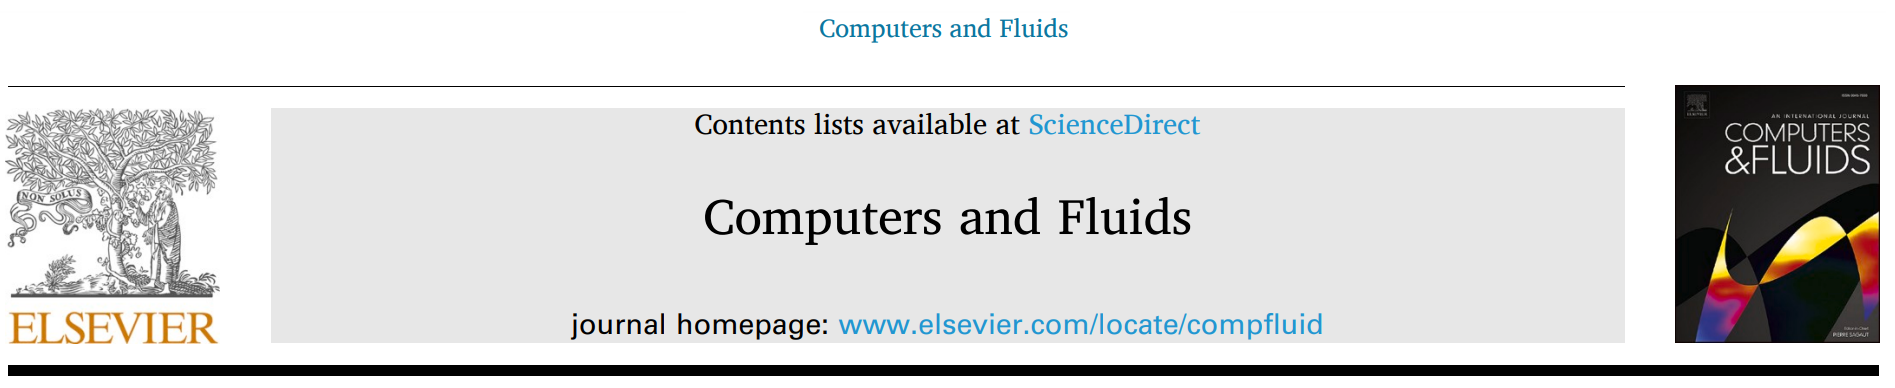
\includegraphics[width=1\linewidth]{headbar_CnF.png}\vspace{0.8cm} Optimizing fluid mixing in channel flow using wall-mounted flexible structures}       
	
	
	\author[1]{Gaurav Singh}[
	%						type=editor,
	%                        auid=000,bioid=1,
	%                        prefix=Sir,
	%                        role=Researcher,
	%                       orcid=0000-0001-7511-2910
	]
	
	%% Corresponding author indication
	\cormark[1]
	%% Footnote of the first author
	%\fnmark[1]
	% Email id of the first author
	\ead{thegauravonline@gmail.com}
	%% URL of the first author
	%\ead[url]{www.cvr.cc, cvr@sayahna.org}
	
	%%  Credit authorship
	%\credit{Conceptualization of this study, Methodology, Software}
	
	% Address/affiliation
	\affiliation[1]{organization={Advanced Technology and Development Centre},
		addressline={Indian Institute of Technology Kharagpur}, 
		city={West Midnapore},
		postcode={721302}, 
		state={W.B.},
		country={India}}
	
	% Fourth author
	%\author[1]{Arahata Senapati}
	\author[1]{Arahata Senapati}
	
	%	\author[3]{Leixin Ma}
	%	%\cormark[2]
	%	%\fnmark[1,3]
	%	%\ead{}
	%	%\ead[URL]{}
	%	%
	%	\affiliation[3]{organization={School for Engineering of Matter, Transport and Energy},addressline={Arizona State University}, 
		%		city={Tempe},
		%		postcode={85281}, 
		%		state={Arizona},
		%		country={USA}}
	
	\author[2]{Arnab Atta}
	%\cormark[2]
	%\fnmark[1,3]
	%\ead{}
	%\ead[URL]{}
	
	\affiliation[2]{organization={Department of Chemical Engineering},
		addressline={Indian Institute of Technology Kharagpur}, 
		city={West Midnapore},
		postcode={721302}, 
		state={W.B.},
		country={India}}
	
	% Third author
	\author[3]{Rajaram Lakkaraju}[%
	%   role=Co-ordinator,
	%   suffix=Jr,
	]
	%\fnmark[2]
	%\ead{}
	%\ead[URL]{}
	\cormark[2]
	\ead{rajaram.lv@gmail.com}
	
	%\credit{Data curation, Writing - Original draft preparation}
	% Address/affiliation
	\affiliation[5]{organization={TuRbulent Interfaces And Dispersion (TRIAD) Group, Department of Mechanical Engineering},
		addressline={Indian Institute of Technology Kharagpur}, 
		city={West Midnapore},
		postcode={721302}, 
		state={W.B.},
		country={India}}
	
	% Corresponding author text
	\cortext[1]{Corresponding author}
	\cortext[2]{Principal corresponding author}
	
	% Here goes the abstract
	\begin{abstract}
		%		Fluid mixing in channel flows is a critical process in various industries, from chemical engineering to food processing. In our study, we focused on a passive mixing method by utilizing flexible wall-mounted plates in a channel of height $h$ at various Reynolds numbers $Re$ to investigate mixing performances. The channel flow we examined involved a scalar field with two initially separated concentration fields, which, upon fluid-structure-scalar interaction, induce agitation and result in the intermixing of the two fields. We have varied the positions of two wall-mounted plates, separated by distance $d=0h-2h$, from each other to form different flow obstructing configurations in the channel, which result in different flow paths, thereby affecting fluid mixing and flow rate due to the pressure head losses. We assessed mixing performance by using two primary metrics: the `Mixing Index' and `Head Loss' along the channel length as cost-benefit analogy. Our results showed that the setup with $d=0$ offers the highest mixing early in the channel length but causes a significant pressure drop. Whereas, a single plate and other two plates separated configurations result in nearly similar levels of mixing for $Re>400$, but head losses increase with decreasing $d$.	
		In channel mixers with two parallel streams of fluid, mixing is achieved by either laminar diffusion at low Reynolds numbers or from flow agitation due to geometric variations. Traditionally, rigid obstructions or textures are used in various spatial arrangements to improve fluid mixing. In our work, we have numerically investigated the mixing performance of a passive scalar in a two-dimensional channel flow accompanied by wall-mounted flexible plates as obstructions for a wide range of low Reynolds numbers ($Re$). The thin plates are arranged on opposite walls of the channel, and the distance between them is varied in the range $0h$ to $2h$, where $h$ is the channel lateral width. The different arrangements result in corresponding flow paths, thereby affecting fluid mixing and flow rate due to the pressure head losses. We assessed the mixing performance in the channel via the mixing index and the head loss. Our results show that the channel with the two plates when arranged exactly opposite the walls (without a separation gap), offers the highest mixing with significant pressure drop. In contrast, either a single plate or two plates widely separated result in nearly similar levels of mixing index with a lower head loss. We devised a performance index based on a cost-benefit analogy by comparing the flexible plate configurations with the plane channel (i.e, without any obstruction) so as to assess the mixing effectiveness and found that a single flexible plate in the channel in the flow conditions with $Re\approx400$ suit the best for the mixing of two fluid in the channel.
		%	Fluid mixing in channel flows is essential in industries like chemical engineering and food processing. Our study utilized two flexible wall-mounted plates in a channel of height \(h\) to investigate mixing at various Reynolds numbers (\(Re\)). The channel flow featured a scalar field with two initially separated concentration fields. Interaction between fluid, structure, and scalar fields induced agitation, leading to intermixing. We varied the positions of the plates, separated by a distance \(d=0h-2h\), to form different obstructing configurations, affecting fluid mixing and flow rate due to pressure head losses. We assessed mixing performance using the 'Mixing Index' and 'Head Loss' along the channel length. Results indicated that the setup with \(d=0\) offered the highest mixing early in the channel but caused significant pressure drops. Conversely, a single plate and other configurations yielded similar mixing levels for \(Re>400\), with head losses increasing as \(d\) is decreased.
		
	\end{abstract}
	
	
	%\linenumbers
	% Use if graphical abstract is present
	% \begin{graphicalabstract}
		% \includegraphics{figs/grabs.pdf}
		% \end{graphicalabstract}
	% Research highlights
	%\begin{highlights}
	%\item Research highlights item 1
	%\item Research highlights item 2
	%\item Research highlights item 3
	%\end{highlights}
	% Keywords
	% Each keyword is separated by \sep
	
	
	\begin{keywords}
		fluid mixing \sep fluid structure interaction \sep flow transition \sep flexible structures \sep vortex generation \sep mixing performance
	\end{keywords}
	
	\maketitle
	
	\setstretch{1}
	\section{Introduction}
	\label{sec:headings}
	
	%%
	
	Fluid mixing is a crucial process in various industries, such as fuel emulsification in petrochemicals, raw material blending in the food industry, and mixing chemical reagents \citep{Yeh2015, Nunez-Flores2020, Peterwitz2021,Wang2021}. To achieve adequate mixing in channel flows, passive methods (like placing obstacles) and active methods (using externally powered actuators) can be employed. Passive methods, such as asymmetric grooves, rigid laminations, and serpentine channels, are simple and energy-efficient as they rely on the flow inertia~\citep{Nguyen2005, Yang_2008, Afzal_2014, Kashid2011, Kang2015,Derksen2010}. Modifying the structural and dimensional aspects of mixing channels can improve mixing outcomes by inducing chaotic convective motions. For instance, \cite{Yang2015} developed a channel design inspired by the three-dimensional Tesla design, demonstrating a robust mixing index of $0.97$ (where $0$ meant no-mixing and $1$ meant perfect-mixing case) within a Reynolds number range of $0.1$ to $100$.

		
	Instead of rigid laminations, the use of flexible plates involves complex interactions between hydrodynamic forces and structural responses, leading to various instabilities~\citep{ Eloy2008, Zhang2000,Taneda1968, Watanabe2002, Alben2008}. These instabilities trigger flow transition by generating eddies in the flow, causing significant improvement in fluid mixing \citep{Self2019,Aaron2019,Self2024}. The incorporation of various vortex-generating methods in mixing channels has emerged as a key approach in enhancing the mixing process \citep{Ali2015,Khatavkar2007,Dadvand2019,Ali2016,Hosseini2021,Ali_2017,Fuchs2011,Derksen2010, Derksen2010, Fuchs2015}. In contrast, for rigid geometry-based vortex generators, the generated vortices primarily remain confined to the small wake region immediately behind the obstacle. This confinement leads to insufficient mixing near the channel walls, particularly when the channel dimensions significantly exceed the size of the obstacle \citep{Wang2020}. A promising solution to this limitation is to employ flexible structures as vortex generators \citep{Hsiao2014,Park2019,Saleh2019,Zhao2020,Chen2020,Nazari_2020,Self_JFS_2024}.
	A crucial method within this approach involves the placement of the obstructions in the flow that act as catalysts for flow agitation \citep{Abdelhamid2021,Yadav2021,Jing2022,Yu2017}. Earlier works \citep{Huarte2011, Borazjani2009, Wang2017} have investigated the flow features when two flexible circular cylinders are placed one after the other. \cite{Wang2017} showed that the two structures act as a single body when placed at small separation, resulting in entirely different flow features when placed at a certain distance. Such strategies have also been used to enhance fluid mixing \citep{Ward2015} and slug mitigation processes \citep{Mehendale2018}.
	
	While experimental methods can measure pressure loss in channel flows, capturing erratic flow and plate motions is challenging, making numerical simulations a preferred approach. Various numerical techniques have been employed in previous studies to simulate fluid-structure interaction problems. In context with the previous works on channel flows, we performed a two-dimensional numerical study to inspect fluid mixing in a channel flow containing two wall-mounted flexible plates mounted on opposite walls. We have systematically varied the position of the two plates to alter the flow features and quantify mixing using standard mixing metrics. We have also investigated the role of the flow Reynolds number that is best suited for efficient mixing conditions. Based on the strong coupling between the flow and the positioned structures, we aim to enhance mixing without causing significant pressure drop. We have focused our study on value (mixing) for cost (head loss) analogy and found the optimal configuration for mixing. In the following sections, we have discussed mathematical formulation, followed by our results and summary.
	%%
		

	\section{Methodology and computational setup}\label{sec:maths}
	
	In Figure \ref{fig:schematic}, we have shown a schematic of our model, a two-dimensional (2D) channel of height $h$ and length $14h$ with two differently dyed fluid flows in the top half and the bottom half of the channel. The channel walls are fixed with flexible plates of length, $l$ $\approx$ $0.5h$ on the opposite wall. The upstream plate is placed at an entry length of $2h$ from the channel inlet, and the second flexible plate is separated at various distances, i.e., $d=0h, 0.5h,1.0h,1.5h, 2.0h$. The thickness and width of each plate are $b = 0.05h$ and $w=0.125h$ (into the plane), respectively. The geometry selected for this study is inspired by our earlier research and a few other similar works \cite{Self2019, Jin2018}, which investigated the flow transition past flexible plates mounted on opposing channel walls. A fully developed flow enters from the left on each dyed half as if the preceding flow had two separate channels with differently dyed fluids. The two flow streams in each half enter through the channel and interact with the wall-mounted structures, generating intricate flow features and thereby causing the mixing of the dyed fluids.
			\begin{figure*}[pos=b]
		\begin{minipage}[c]{1\linewidth}	
			%		\begin{overpic}[width=1\linewidth]{Figures/fig1a.png}
				\begin{overpic}[width=1\linewidth]{Figures/3_a2.png}
					%			\put(280,148){{\parbox{1\linewidth}{$\phi = 1$}}}	
					%			\put(280,123){{\parbox{1\linewidth}{$\phi = 0$}}}	
					%			\put(80,-2){{\parbox{1\linewidth}{$Re/Re_s$}}}	
					%			\put(20,52){{\parbox{1\linewidth}{\rotatebox{90}{$y/h$}}}}	
				\end{overpic}
			\end{minipage}
			%		\vspace{-0.2cm}
			\caption{Schematic of a flow in a channel with a scalar concentration field $\phi$, separated along the channel length in the top half as $\phi=0$ and bottom half as $\phi=1$. The channel walls consist of oppositely mounted flexible plates that bend in the streamwise direction when flow enters from the inlet (left). The inlet flow profile is considered fully developed separately for both the top-half and bottom-half concentration fields as if they enter the domain from two different sources. Plate 1 and plate 2, each of height $0.5h$, are separated at different distances ($d/h$).}
			\label{fig:schematic}
		\end{figure*}\vspace{0cm}
	We have conducted a fluid-structure interaction numerical simulation for the mentioned domain using a partitioned approach, in which the fluid domain and the structure domain are numerically solved separately, and solutions are then exchanged to set iterative boundary conditions at the interface. We have considered fluid as Newtonian and incompressible, mathematically formulated by the Navier-Stokes equations. The linearly elastic structure is framed as solid equations of motion formulated using Arbitrary Lagrangian-Eulerian (ALE) framework~\cite{Nguyen2010, Slone2002, CampbellPaterson2011}. The mass and momentum conservation expressions for the fluid and the structure are as follows,
	\begin{center}\vspace{-0.5cm}
		\begin{equation}
			\nabla\cdot\left[(\mathbf{u}_f-\mathbf{u}_m)\right] = 0,
		\end{equation}
		\begin{equation}
			{\partial\mathbf{u}_f\over\partial t} + \left[(\mathbf{u}_f-\mathbf{u}_m) \cdot\mathbf{\nabla}\right]\mathbf{u}_f = -\nabla p+\frac{1}{Re}\nabla^2\mathbf{u}_f
		\end{equation}
		\begin{equation}
			\rho_s{\partial^2\mathbf{u}_s\over\partial t^2} = \mathbf{\nabla}\cdot\mathbf{\boldsymbol{\sigma}}_s
		\end{equation}
	\end{center}
	
	Here, $\mathbf{u}_f=(u_x,u_y)$ denotes the flow velocity, while $\mathbf{u}_m$ stands for the moving mesh velocity, and $p$ represents the pressure, $\rho_s$ symbolizes the structure density, $\mathbf{u}_s$ is the structural displacement, $t$ is time, and the Cauchy stress tensor is represented by $\sigma_s$. $\frac{\partial}{\partial t}$ indicates the time derivative operator, and the spatial gradient is defined as $\nabla\equiv\left(\frac{\partial}{\partial x},\frac{\partial}{\partial y}\right)$, with $\nabla^2$ representing the Laplacian operator. The Reynolds number, $Re$, is defined as $Re=\overline{U}h/\nu_f$, where $\overline{U}$ is the vertical mean inlet flow velocity and $\nu_f$ ($=\mu_f/\rho_f$) is the fluid's kinematic viscosity. The subscripts $_f$, $_s$, and $_m$ refer to fluid, solid, and mesh, respectively.
	
	When the plates deform under the fluid load, the strain rate is expressed as $\boldsymbol{\varepsilon}_s={1\over2}(\mathbf{\nabla}\mathbf{u}_s+\mathbf{\nabla}\mathbf{u}_s^T+\mathbf{\nabla}\mathbf{u}_s \cdot \mathbf{\nabla}\mathbf{u}_s^T)$. The relationship between the stress and strain tensors is given by $\boldsymbol{\sigma}_s=2\mu_s \boldsymbol{\varepsilon}_s+\lambda( \mathbf{\nabla}\cdot\mathbf{u}_s)\mathcal{I}$, where $\mu_s=\mathcal{E}/[2(1+\kappa)]$ and $\lambda=\kappa \mathcal{E}/[(1+\kappa)(1-2\kappa)]$ are Lame's constants. Here, $\kappa$ denotes the Poisson's ratio, $\mathcal{E}$ is Young's modulus, and $\mathcal{I}$ is the identity tensor of rank two. The transpose of a tensor is indicated by the superscript $^T$. The interface condition ensures that flow stress and structural displacement influence each other through no-slip boundary conditions, and the mesh velocity is assumed to be equal to the structure velocity, i.e., $\mathbf{u}_m\equiv {\partial\mathbf{u}_s\over\partial t}$.
	
			\begin{figure*}[pos=b!]
		\begin{center}
			\begin{minipage}[c]{0.33\linewidth}	
				\centering	
				\begin{overpic}[width=1\linewidth]{Figures/delta_Re200_1600_single2.png}
					\put(0,138){{\parbox{1\linewidth}{$(a)$}}}
				\end{overpic}
			\end{minipage}  
			\begin{minipage}[c]{0.32\linewidth}	
				\centering		
				\begin{overpic}[width=1\linewidth]{Figures/1.eps}
					\put(0,137){{\parbox{1\linewidth}{$(b)$}}}
				\end{overpic}
			\end{minipage}
			\begin{minipage}[c]{0.32\linewidth}	
				\centering	
				\begin{overpic}[width=1\linewidth]{Figures/2.eps}
					\put(5,137){{\parbox{1\linewidth}{$(c)$}}}
				\end{overpic}
			\end{minipage}
		\end{center}
		\vspace{-15px}
		\caption{(a) Time history of the single plate tip deflection about steady state mean position for $Re=200$ and $1600$. A stroboscopic representation of the bending plate is shown in the inset figure, and the thick red plate marks the steady-state shape after deflection. (b) Tip deflection normalized by single plate mean deflection of plate 1 (upstream) and (c) plate 2 for different $d/h$ configurations. The dashed line marks the single plate tip deflection for reference. The inset in each panel shows a tip deflection trend with $d/h$ for $Re=200$ and $3200$.}
		\label{fig:del_g_vs_Ca_steady}
	\end{figure*}
	
	In the presented setup, we have added a scalar concentration field $\phi$ to simulate the dyed fluids effect. The dye concentration fields follow the advection-diffusion equation as,
%	\begin{equation}
%		{\partial\phi\over\partial t}+(\mathbf{u}_f-\mathbf{u}_m)\cdot\mathbf{\nabla}\mathbf{\phi} = \frac{1}{Re\cdot Sc}\nabla^2\mathbf{\phi},
%	\end{equation}
%	where $\phi$ is the scalar concentration field ranging from 0 to 1, and $Sc=\nu_f/D$ is the Schmidt number with $D$ as the mass diffusivity constant. 	
	We used the finite-volume method to solve the mentioned governing equations by employing a second-order accurate Euler-implicit scheme for temporal discretization and a second-order vanLeer TVD scheme for spatial discretization of convection terms. For diffusion terms, we applied a central differencing scheme with Gaussian integration. We maintained the Courant number below 0.2, calculated based on the local velocity magnitude, the integration time step, and the length of the computational cell. Our solution method involves predicting the interface displacement and computing the initial interface residual. This entails estimating the movement of the interface between the fluid and structure domains and determining the deviation from its initial position. After calculating the initial interface residual, the algorithm begins the fluid-structure interaction using a strongly coupled iterative procedure until the convergence criterion is achieved ~\citep{Hrvoje2007, CampbellPaterson2011}. This iterative process is repeated under the Aitken dynamic relaxation approach until the desired tolerance level is achieved.
		
		
	In our study, we denote the characteristic velocity by $\overline{U}$ and define the characteristic length as the flow gap between the wall and the wall-mounted plate, which is $(h - l) = 0.5h$ ($= l$). The dimensionless parameters include the Reynolds number $Re=\overline{U}l/\nu_f$, the density ratio $\rho_s/\rho_f$, and Cauchy number as the ratio of fluid inertia to elastic restoring force i.e. $Ca=\rho_f \overline{U}^2 h^3 b/{\mathcal{E}I}$, where $I=bw^3/12$ is the plate's area moment of inertia \citep{Bhageri2012,Pinelli2015}. Another critical parameter is the dimensionless gap between the plates, $d/h$. Our study primarily involves two time scales: (1) the plate's elasticity time scale, $\tau \sim{1/\sqrt{\mathcal{E}I/(\rho_s bwl^4)}}$, and (2) the convective motion time scale, $T \sim l/v_{\infty}$. When $\tau/T$ is much less than 1, the plate shows oscillations at its natural frequency due to the negligible fluid inertia. Conversely, when $\tau/T$ is much greater than 1, fluid inertia dominates the plate's oscillations. Notably, $\tau$ and $Ca$ are related through $\tau \sim \sqrt{\left({\rho_s w/\rho_f h}\right)Ca}$. Given the significance of elastic restoring forces, we selected a small $Ca$ value ($\approx 0.015$) to align with previous studies involving flexible silicone obstructions~\citep{Vandenberghe2004, Self2019}. Our main objective is to examine fluid mixing by varying the inlet Reynolds number within the range $100 < Re < 3200$ and adjusting the plate separation gap from $0h$ to $2h$.
		

		
		The velocity boundary conditions applied to the channel walls and flexible structure surfaces are no-slip and impermeable. At the channel outlet, the velocity gradients are set to zero, while the inlet velocity follows a parabolic inflow profile for both the top and bottom half, as previously described. The velocity at the interface between the solid structure and the fluid is the same, i.e., a no-slip boundary condition is used. Pressure boundary conditions are set to zero gradients at the channel walls, inlet, fluid-solid interface, and ambient pressure conditions at the outlet. Our study focuses on the streamwise location $x=12h$, ensuring no boundary reflections and allowing properties to stabilize before exiting the channel.
		
		\section{Results}
		
		We have investigated the fluid mixing in a channel flow due to the passively oscillating flexible plates. According to \cite{Zhang2020}, such plates subjected to an incoming flow may exhibit different deformation modes: lodging mode, regular VIV mode (vortex-induced vibration or flutter), or static reconfiguration mode. Our parameter range places our cases in the phase space that shows static reconfiguration of the plates, as described in \cite{Zhang2020}, where the plates align with the flow, reducing the projected area perpendicular to the flow and showing negligible flutter at steady-state.
		
		To begin with, we studied the behavior of the flexible plates under the incoming flow. 
		In Figure \ref{fig:del_g_vs_Ca_steady}(a), we have shown the plates' flutter oscillation for the case where only a single plate is positioned at $2h$ length from the channel inlet. This plate reconfigures by bending in the streamwise direction by amplitude $\overline{\delta}_s$ and flutters around its mean position (shown as plate position in red in the subplot). The plates' flutter amplitude dampens down smoothly for $Re=200$, unlike that in the high $Re ~(=1600)$ case where the plates' flutter shows abrupt dampening due to flow features. We have also shown the mean plate deflection for increasing $Re$ in the subplot, which shows a nearly linear trend in the semi-log plot. In the case with two wall-mounted plates arrangement, Figure \ref{fig:del_g_vs_Ca_steady}(b) and (c) show steady state deflection amplitude for upstream plate ($\overline{\delta}_1$) and for the downstream plate ($\overline{\delta}_2$) normalized over the deflection amplitude in single plate case ($\overline{\delta}_S$). We can observe that the $\overline{\delta}_1 > \overline{\delta}_S)$ for any $Re$ and $d/h$ case whereas $\overline{\delta}_2 > \overline{\delta}_S)$ $for d/h>0.8$. We have also shown the normalized plate deflection for $d/h$ cases in the subfigures and found that the plate deflection increases with a decrease in $d/h$. We have thoroughly discussed the structural dynamics of the wall-mounted plates' such as damping, frequency, and deflection, in detail in our earlier work \citep{Self2019}.
		
		\begin{figure*}[]
			\begin{minipage}[c]{0.45\linewidth}		
				\begin{overpic}[trim={0.1cm 0 15cm 0},clip,width=1\linewidth]{Figures/vort_Single_a_4000.png}
					\put(-36,12){{\parbox{1\linewidth}{$Re$=$200$}}}
				\end{overpic}\vspace{-0.15cm}
				\begin{overpic}[trim={0.1cm 0 15cm 0},clip,width=1\linewidth]{Figures/vort_Single_b_4000.png}
					\put(-36,12){{\parbox{1\linewidth}{$Re$=$400$}}}
				\end{overpic}\vspace{-0.15cm}
				\begin{overpic}[trim={0.1cm 0 15cm 0},clip,width=1\linewidth]{Figures/vort_Single_c_4000.png}
					\put(-36,12){{\parbox{1\linewidth}{$Re$=$800$}}}
				\end{overpic}\vspace{-0.15cm}
				\begin{overpic}[trim={0.1cm 0 15cm 0},clip,width=1\linewidth]{Figures/vort_Single_d_4000.png}
					\put(-36,12){{\parbox{1\linewidth}{$Re$=$1600$}}}
				\end{overpic}\vspace{-0.15cm}
				\begin{overpic}[trim={0.1cm 0 15cm 0},clip,width=1\linewidth]{Figures/vort_Single_e_4000.png}
					\put(-36,12){{\parbox{1\linewidth}{$Re$=$3200$}}}
				\end{overpic}\vspace{0.5cm}
			\end{minipage} 
			\begin{minipage}[c]{0.48\linewidth}		
				\begin{overpic}[trim={1cm 0 15cm 0},clip,width=1\linewidth]{Figures/T2_Single_a_4000.png}
					\put(-225,28){{\parbox{1\linewidth}{$(a)$}}}	
					\put(0,28){{\parbox{1\linewidth}{$(b)$}}}
				\end{overpic}\vspace{-0.15cm}
				\begin{overpic}[trim={1cm 0 15cm 0},clip,width=1\linewidth]{Figures/T2_Single_b_4000.png}
				\end{overpic}\vspace{-0.15cm}
				\begin{overpic}[trim={1cm 0 15cm 0},clip,width=1\linewidth]{Figures/T2_Single_c_4000.png}
				\end{overpic}\vspace{-0.15cm}
				\begin{overpic}[trim={1cm 0 15cm 0},clip,width=1\linewidth]{Figures/T2_Single_d_4000.png}
				\end{overpic}\vspace{-0.15cm}
				\begin{overpic}[trim={1cm 0 15cm 0},clip,width=1\linewidth]{Figures/T2_Single_e_4000.png}
					%			\put(180,-5){{\parbox{1\linewidth}{$Single$}}}
					\put(-104,-16){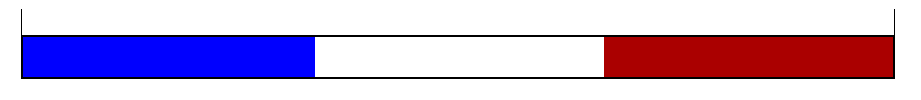
\includegraphics[width=0.15\linewidth]{Figures/legend_vortex.png}}
					\put(136,-16){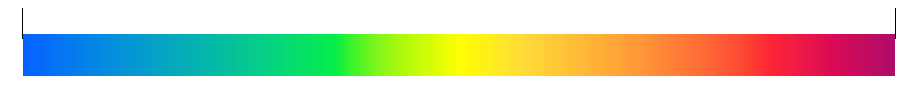
\includegraphics[width=0.15\linewidth]{Figures/legend_scalar.png}}
					\put(-110,-6){{\parbox{1\linewidth}{$-\infty$}}}	
					\put(-82,-6){{\parbox{1\linewidth}{\small$-10$}}}
					\put(-12,-6){{\parbox{1\linewidth}{$\infty$}}}	
					\put(-43,-6){{\parbox{1\linewidth}{\small$10$}}}
					\put(-60,-6){{\parbox{1\linewidth}{\large$\omega_z$}}}
					\put(132,-6){{\parbox{1\linewidth}{$0$}}}
					\put(232,-6){{\parbox{1\linewidth}{$1$}}}
					\put(183,-6){{\parbox{1\linewidth}{$\phi$}}}
				\end{overpic}\vspace{0.5cm}
			\end{minipage}
			%	\vspace{0.1cm}
			\caption{Instantaneous (a) iso-contours of spanwise vorticity ($\omega_z$) and (b) scalar concentration field for single plate configuration case. The top-to-bottom panels are for $Re=200$ to $3200$.}
			\label{fig:contour_single}
		\end{figure*}
		
		
		\begin{figure}[b]
			\begin{minipage}[c]{0.495\linewidth}
				%			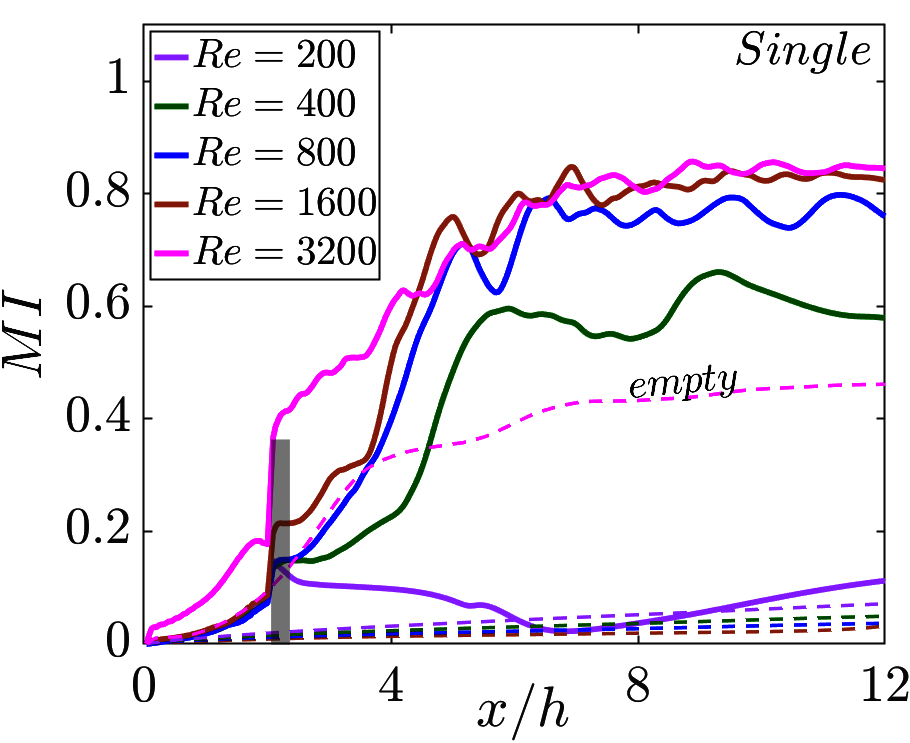
\includegraphics[width=1\linewidth,trim={0cm 0 0 0},clip]{Figures/MI_HL/MI_x_single_46.png}
				\begin{overpic}[width=1\linewidth,trim={0cm 0 0 0},clip]{Figures/MI_HL/MI_x_single_46.png}
					\put(4,96){{\parbox{1\linewidth}{$(a)$}}}	
				\end{overpic}
			\end{minipage}
			\begin{minipage}[c]{0.495\linewidth}		
				\begin{overpic}[width=1\linewidth,trim={0cm 0 0 0},clip]{Figures/MI_HL/HL_x_single_46.png}
					\put(-1,96){{\parbox{1\linewidth}{$(b)$}}}
				\end{overpic}
			\end{minipage}  
			
			%	\vspace{0.5cm}
			\caption{Time-averaged (a) mixing index $MI$ and (b) head loss $HL$ along the channel length downstream for a single flexible plate case for $Re=200-3200$. The grey rectangle marks the location of plates in the channel. The dashed lines correspond to the empty channel case for respective $Re$ as per the color code.}
			\label{fig:MI_Single}
		\end{figure}
		
		
		\begin{figure*}[]
			\begin{minipage}[c]{0.45\linewidth}		
				\begin{overpic}[trim={0.1cm 0 15cm 0},clip,width=1\linewidth]{Figures/vort_Single_b_4000.png}
					\put(-32,12){{\parbox{1\linewidth}{$Single$}}}
				\end{overpic}\vspace{-0.15cm}
				\begin{overpic}[trim={0.1cm 0 15cm 0},clip,width=1\linewidth]{Figures/vort_4_b_4000.png}
					\put(-34,12){{\parbox{1\linewidth}{$d/h$=$2.0$}}}
				\end{overpic}\vspace{-0.15cm}
				\begin{overpic}[trim={0.1cm 0 15cm 0},clip,width=1\linewidth]{Figures/vort_3_b_4000.png}
					\put(-34,12){{\parbox{1\linewidth}{$d/h$=$1.5$}}}
				\end{overpic}\vspace{-0.15cm}
				\begin{overpic}[trim={0.1cm 0 15cm 0},clip,width=1\linewidth]{Figures/vort_2_b_4000.png}
					\put(-34,12){{\parbox{1\linewidth}{$d/h$=$1.0$}}}
				\end{overpic}\vspace{-0.15cm}
				\begin{overpic}[trim={0.1cm 0 15cm 0},clip,width=1\linewidth]{Figures/vort_1_b_4000.png}
					\put(-34,12){{\parbox{1\linewidth}{$d/h$=$0.5$}}}
				\end{overpic}\vspace{-0.15cm}
				\begin{overpic}[trim={0.1cm 0 15cm 0},clip,width=1\linewidth]{Figures/vort_0_b_4000.png}
					\put(-34,12){{\parbox{1\linewidth}{$d/h$=$0.0$}}}
				\end{overpic}\vspace{0.5cm}
			\end{minipage} 
			\begin{minipage}[c]{0.48\linewidth}		
				\begin{overpic}[trim={1cm 0 15cm 0},clip,width=1\linewidth]{Figures/T2_Single_b_4000.png}
				\end{overpic}\vspace{-0.15cm}
				\begin{overpic}[trim={1cm 0 15cm 0},clip,width=1\linewidth]{Figures/T2_4_b_4000.png}
					\put(-225,56){{\parbox{1\linewidth}{$(a)$}}}	
					\put(0,56){{\parbox{1\linewidth}{$(b)$}}}
				\end{overpic}\vspace{-0.15cm}
				\begin{overpic}[trim={1cm 0 15cm 0},clip,width=1\linewidth]{Figures/T2_3_b_4000.png}
				\end{overpic}\vspace{-0.15cm}
				\begin{overpic}[trim={1cm 0 15cm 0},clip,width=1\linewidth]{Figures/T2_2_b_4000.png}
				\end{overpic}\vspace{-0.15cm}
				\begin{overpic}[trim={1cm 0 15cm 0},clip,width=1\linewidth]{Figures/T2_1_b_4000.png}
				\end{overpic}\vspace{-0.15cm}
				\begin{overpic}[trim={1cm 0 15cm 0},clip,width=1\linewidth]{Figures/T2_0_b_4000.png}
					% \put(180,-5){{\parbox{1\linewidth}{$Single$}}}
					\put(-104,-17){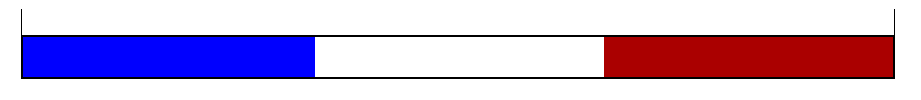
\includegraphics[width=0.15\linewidth]{Figures/legend_vortex.png}}
					\put(136,-17){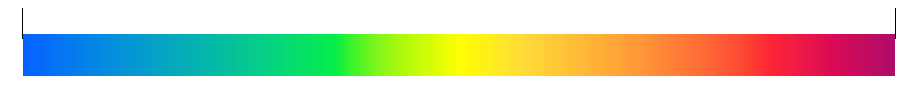
\includegraphics[width=0.15\linewidth]{Figures/legend_scalar.png}}
					%			\put(-110,-2.5){{\parbox{1\linewidth}{$-\infty$}}}	
					%			\put(-80,-2.5){{\parbox{1\linewidth}{$-10$}}}
					%			\put(-12,-3){{\parbox{1\linewidth}{$\infty$}}}	
					%			\put(-43,-3){{\parbox{1\linewidth}{$10$}}}
					%			\put(-59,-4){{\parbox{1\linewidth}{\large$\omega_z$}}}
					%			\put(125,-2.5){{\parbox{1\linewidth}{$0$}}}
					%			\put(219,-2.5){{\parbox{1\linewidth}{$1$}}}
					%			\put(170,-3){{\parbox{1\linewidth}{$\phi$}}}
					\put(-110,-7.5){{\parbox{1\linewidth}{$-\infty$}}}	
					\put(-82,-7.5){{\parbox{1\linewidth}{\small$-10$}}}
					\put(-12,-7.5){{\parbox{1\linewidth}{$\infty$}}}	
					\put(-43,-7.5){{\parbox{1\linewidth}{\small$10$}}}
					\put(-60,-7){{\parbox{1\linewidth}{\large$\omega_z$}}}
					\put(132,-6){{\parbox{1\linewidth}{$0$}}}
					\put(232,-6){{\parbox{1\linewidth}{$1$}}}
					\put(183,-6){{\parbox{1\linewidth}{$\phi$}}}
				\end{overpic}\vspace{0.5cm}
			\end{minipage}
			%	\vspace{0.1cm}
			\caption{Instantaneous (a) iso-contours of spanwise vorticity ($\omega_z$) and (b) scalar concentration field for $Re=800$ case. The top-to-bottom panels are for different $d/h$ configurations. A full animation is provided as the supplementary \citep{animation} for all $Re$ cases.}
			\label{fig:contour_800}
		\end{figure*}
		
		
		\begin{figure*}[t]
			\begin{minipage}[c]{0.495\linewidth}
				%			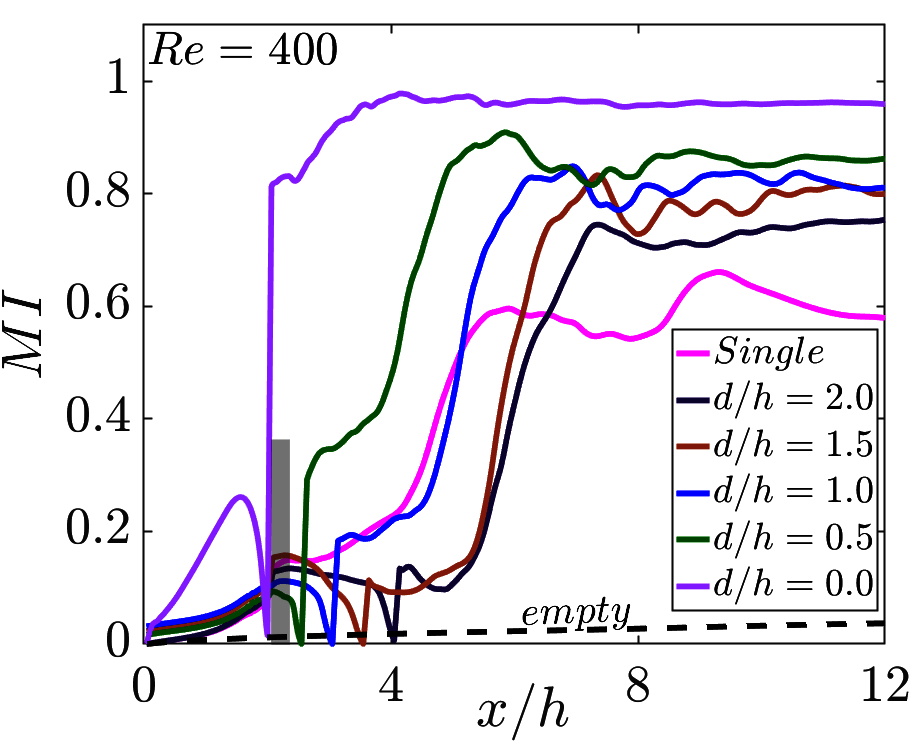
\includegraphics[width=1\linewidth,trim={0cm 0 0 0},clip]{Figures/MI_HL/MI_x_Re400_46.png}
				\begin{overpic}[width=1\linewidth,trim={0cm 0 0 0},clip]{Figures/MI_HL/MI_x_Re400_46.png}
					\put(0,186){{\parbox{1\linewidth}{$(a)$}}}	
				\end{overpic}
			\end{minipage}
			\begin{minipage}[c]{0.495\linewidth}		
				\begin{overpic}[width=1\linewidth,trim={0cm 0 0 0},clip]{Figures/MI_HL/HL_x_Re400_46.png}
					\put(0,186){{\parbox{1\linewidth}{$(b)$}}}
				\end{overpic}
			\end{minipage}
			%	\vspace{0.5cm}
			\caption{Time-averaged (a) mixing index $MI$ and (b) head loss $HL$ along the channel length in the downstream for single and two plate cases with different $d/h$ configurations at $Re=400$. The grey rectangle marks the location of plates in the channel. The dashed lines correspond to the empty channel case for respective $Re$ as per the color code.}
			\label{fig:MI_400}
		\end{figure*}
		
		\begin{figure*}[t]
			\vspace{0cm}
			\begin{minipage}[c]{0.24\linewidth}
				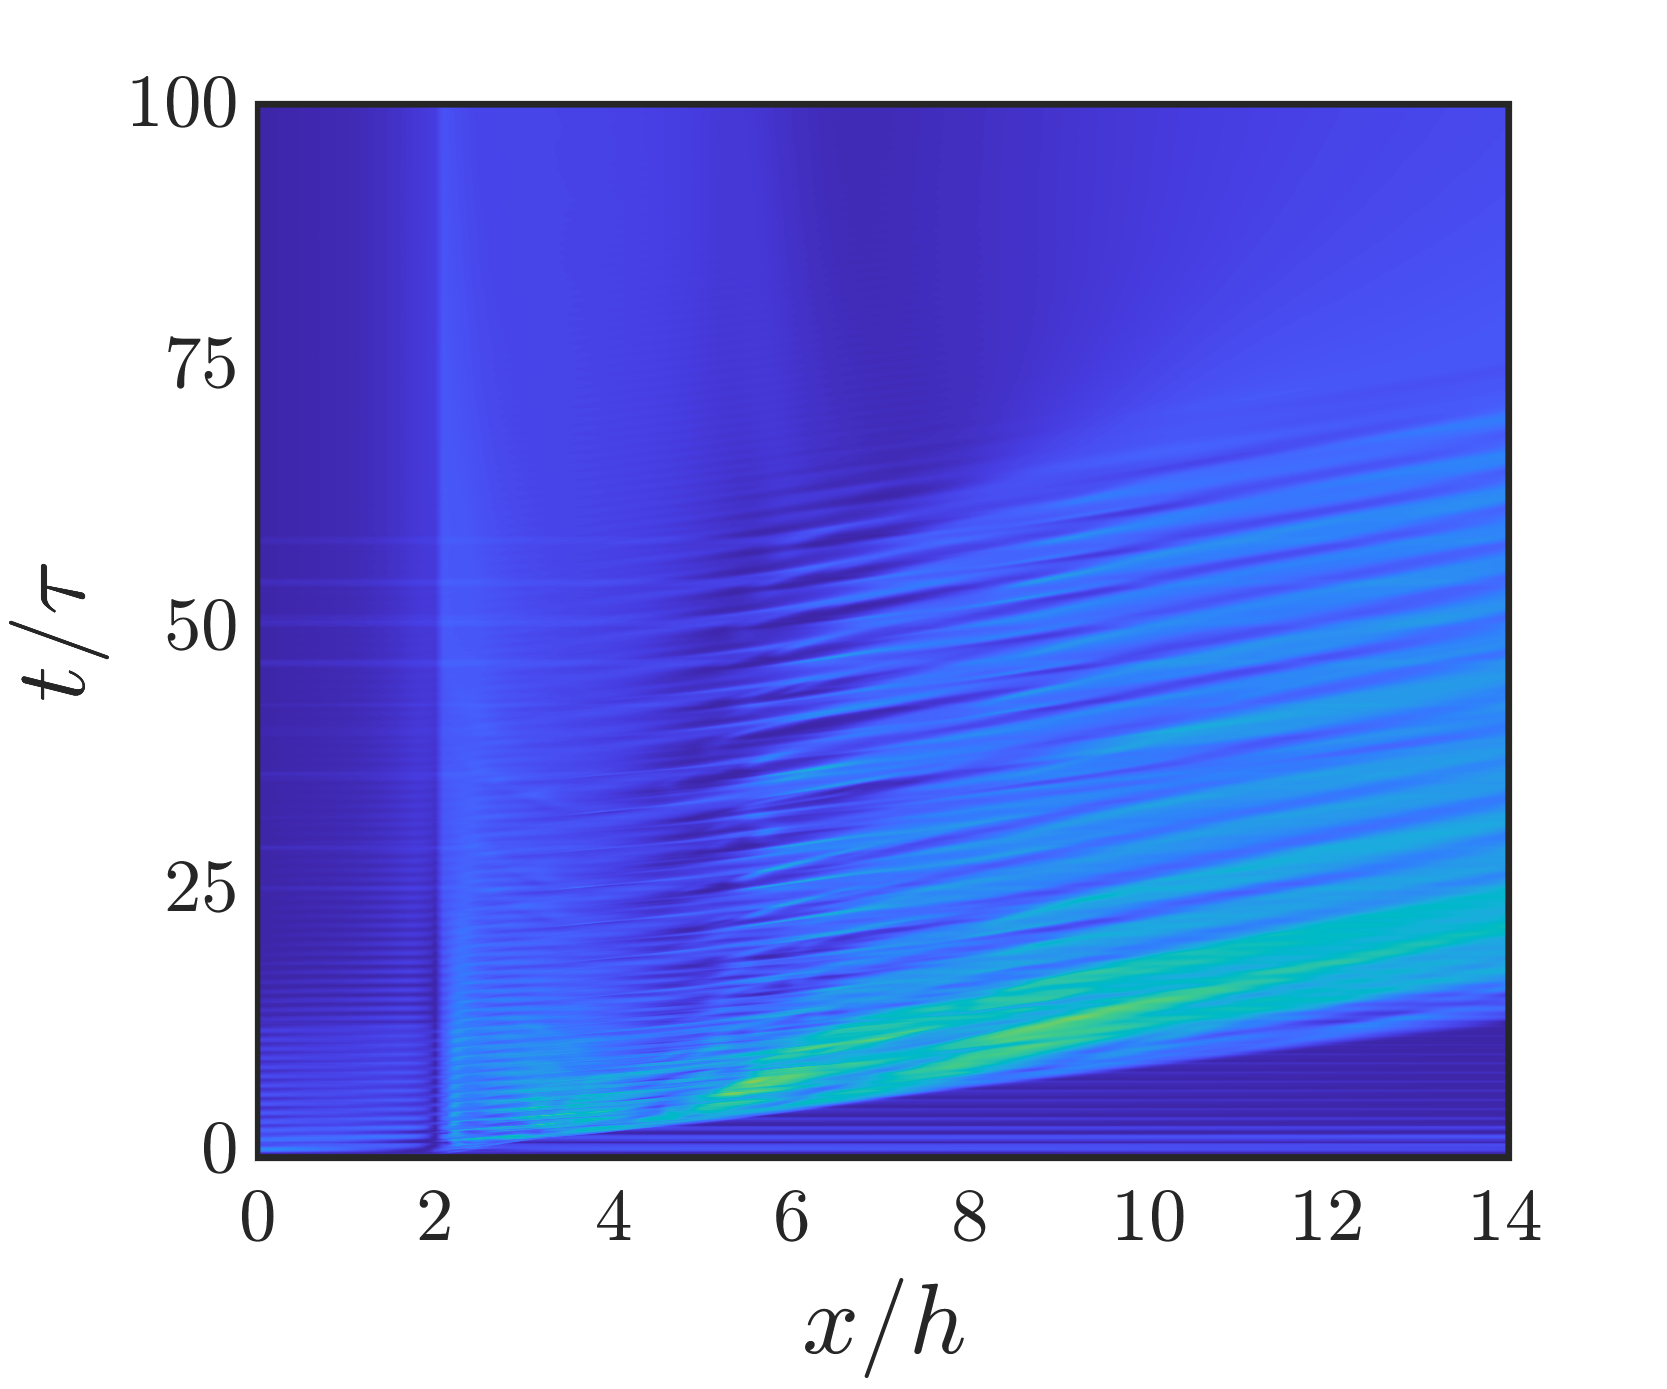
\includegraphics[width=1\linewidth,trim={1.6cm 2cm 2cm 1cm},clip]{Figures/MI_HL/spcaeTime_M_Singlea.png}
				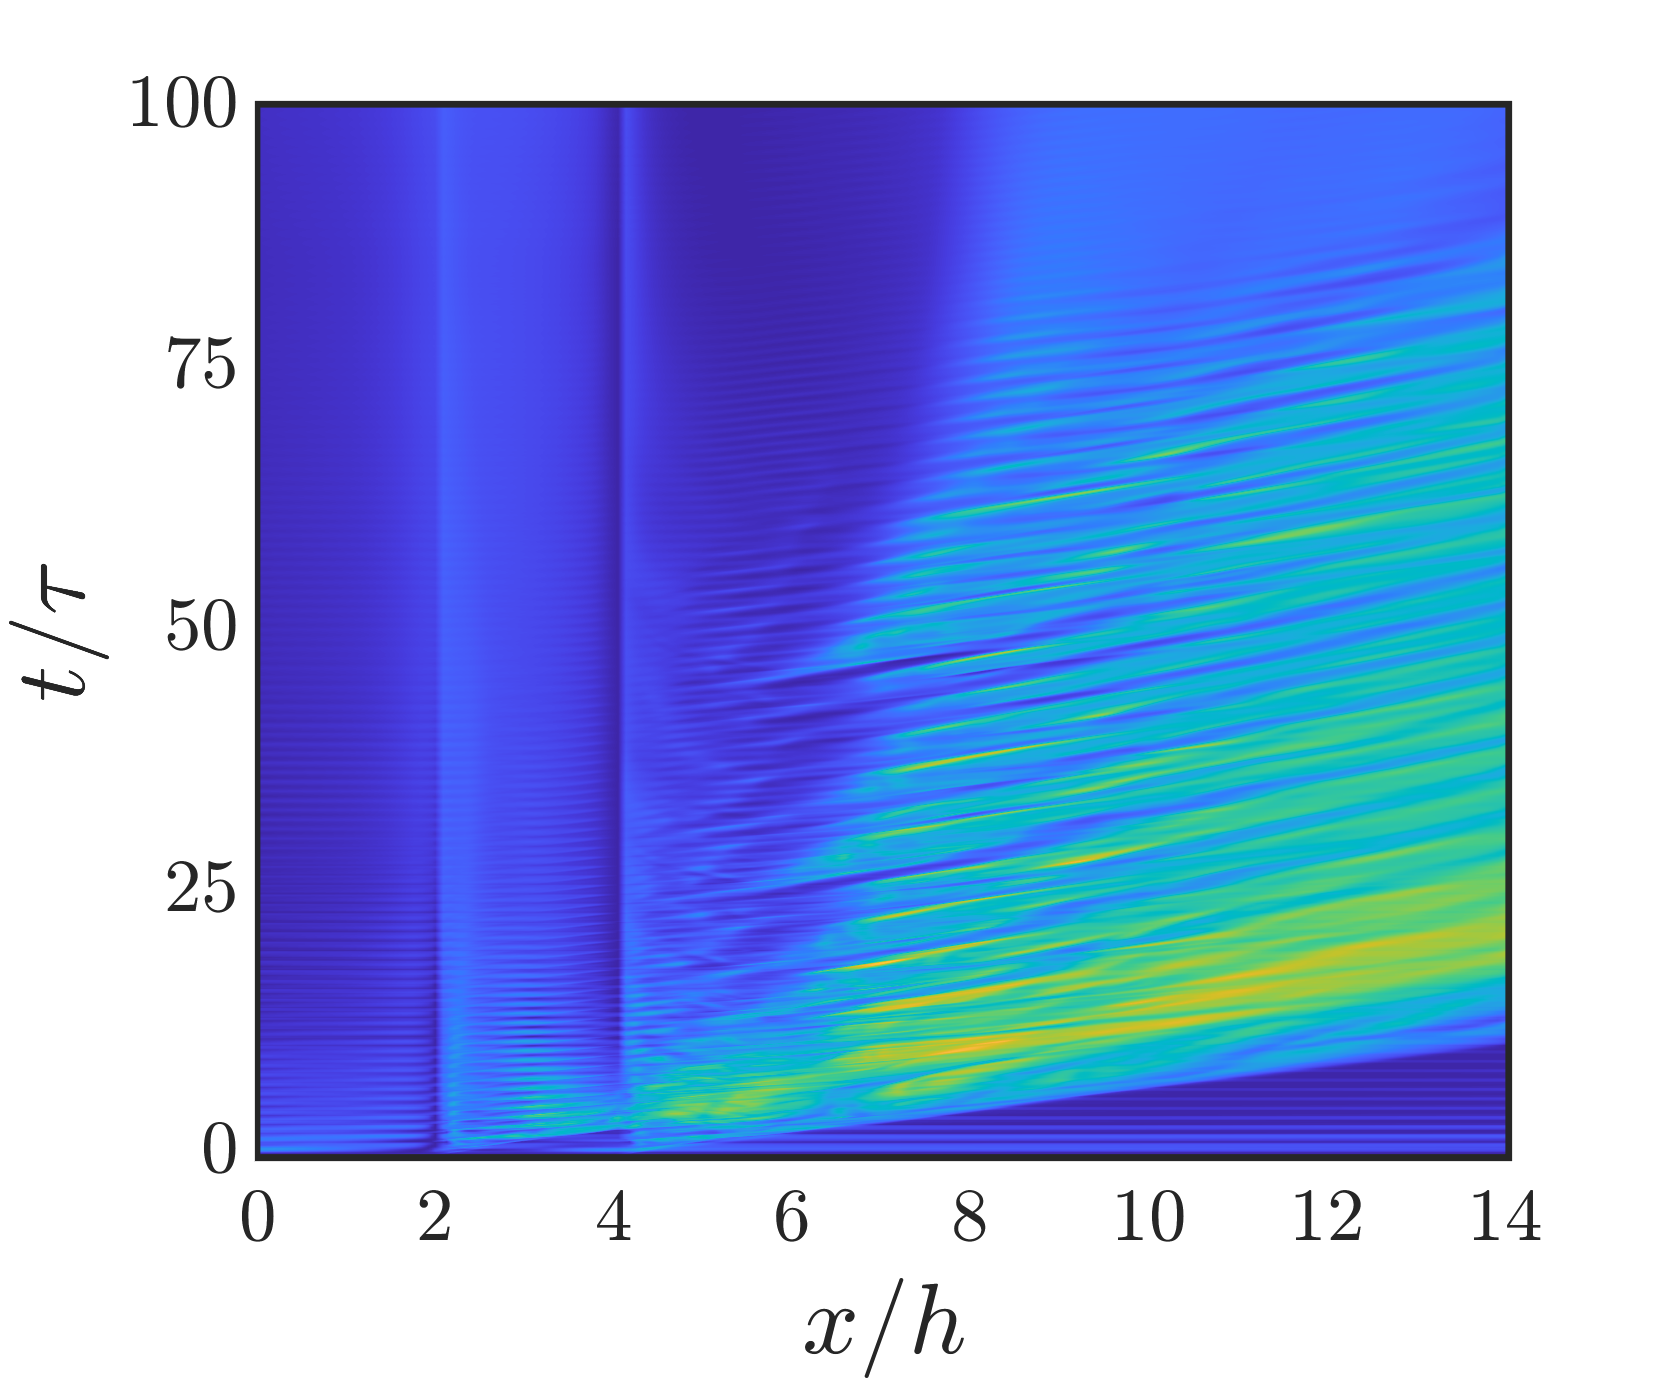
\includegraphics[width=1\linewidth,trim={1.6cm 2cm 2cm 1cm},clip]{Figures/MI_HL/spcaeTime_M_4a.png}
				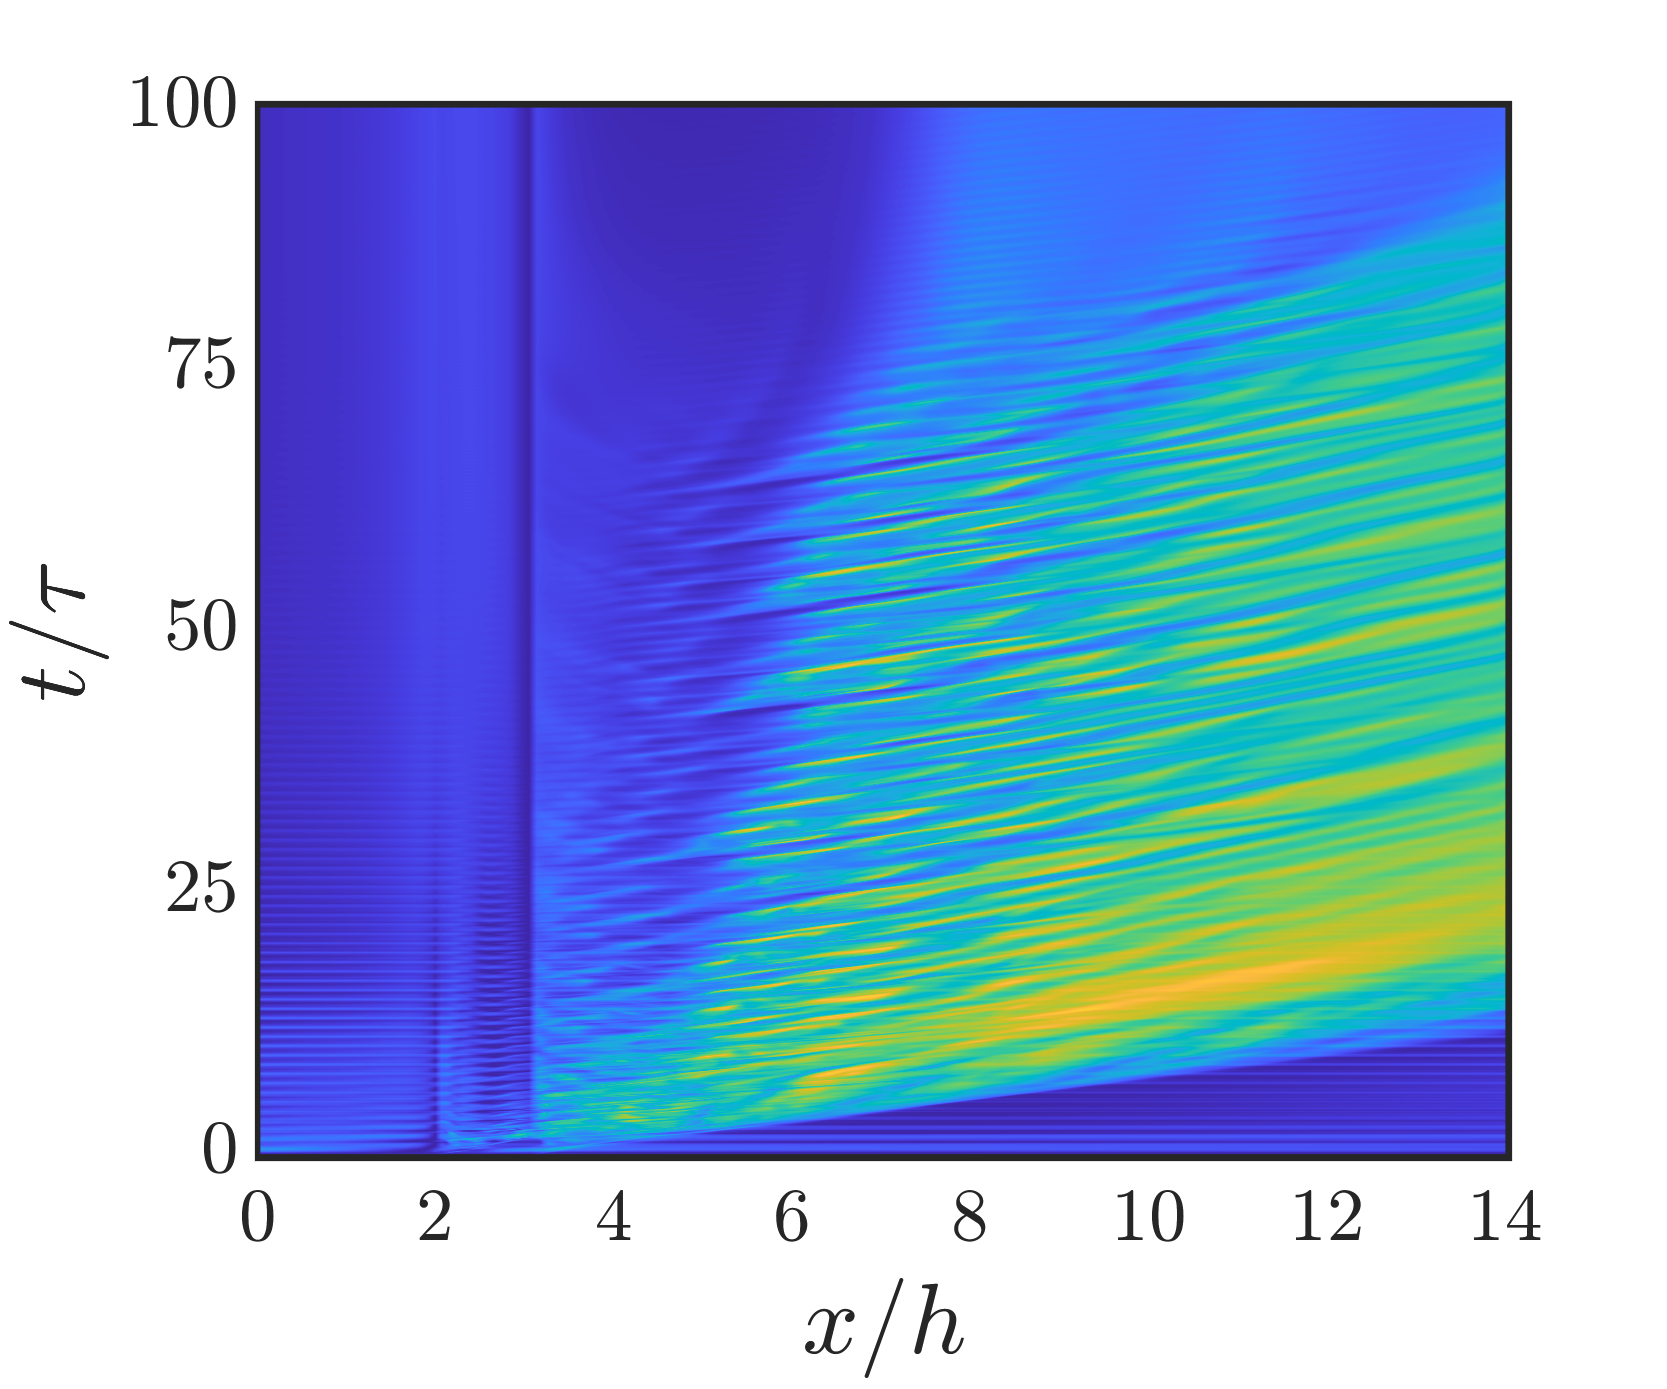
\includegraphics[width=1\linewidth,trim={1.6cm 2cm 2cm 1cm},clip]{Figures/MI_HL/spcaeTime_M_2a.png}
				%		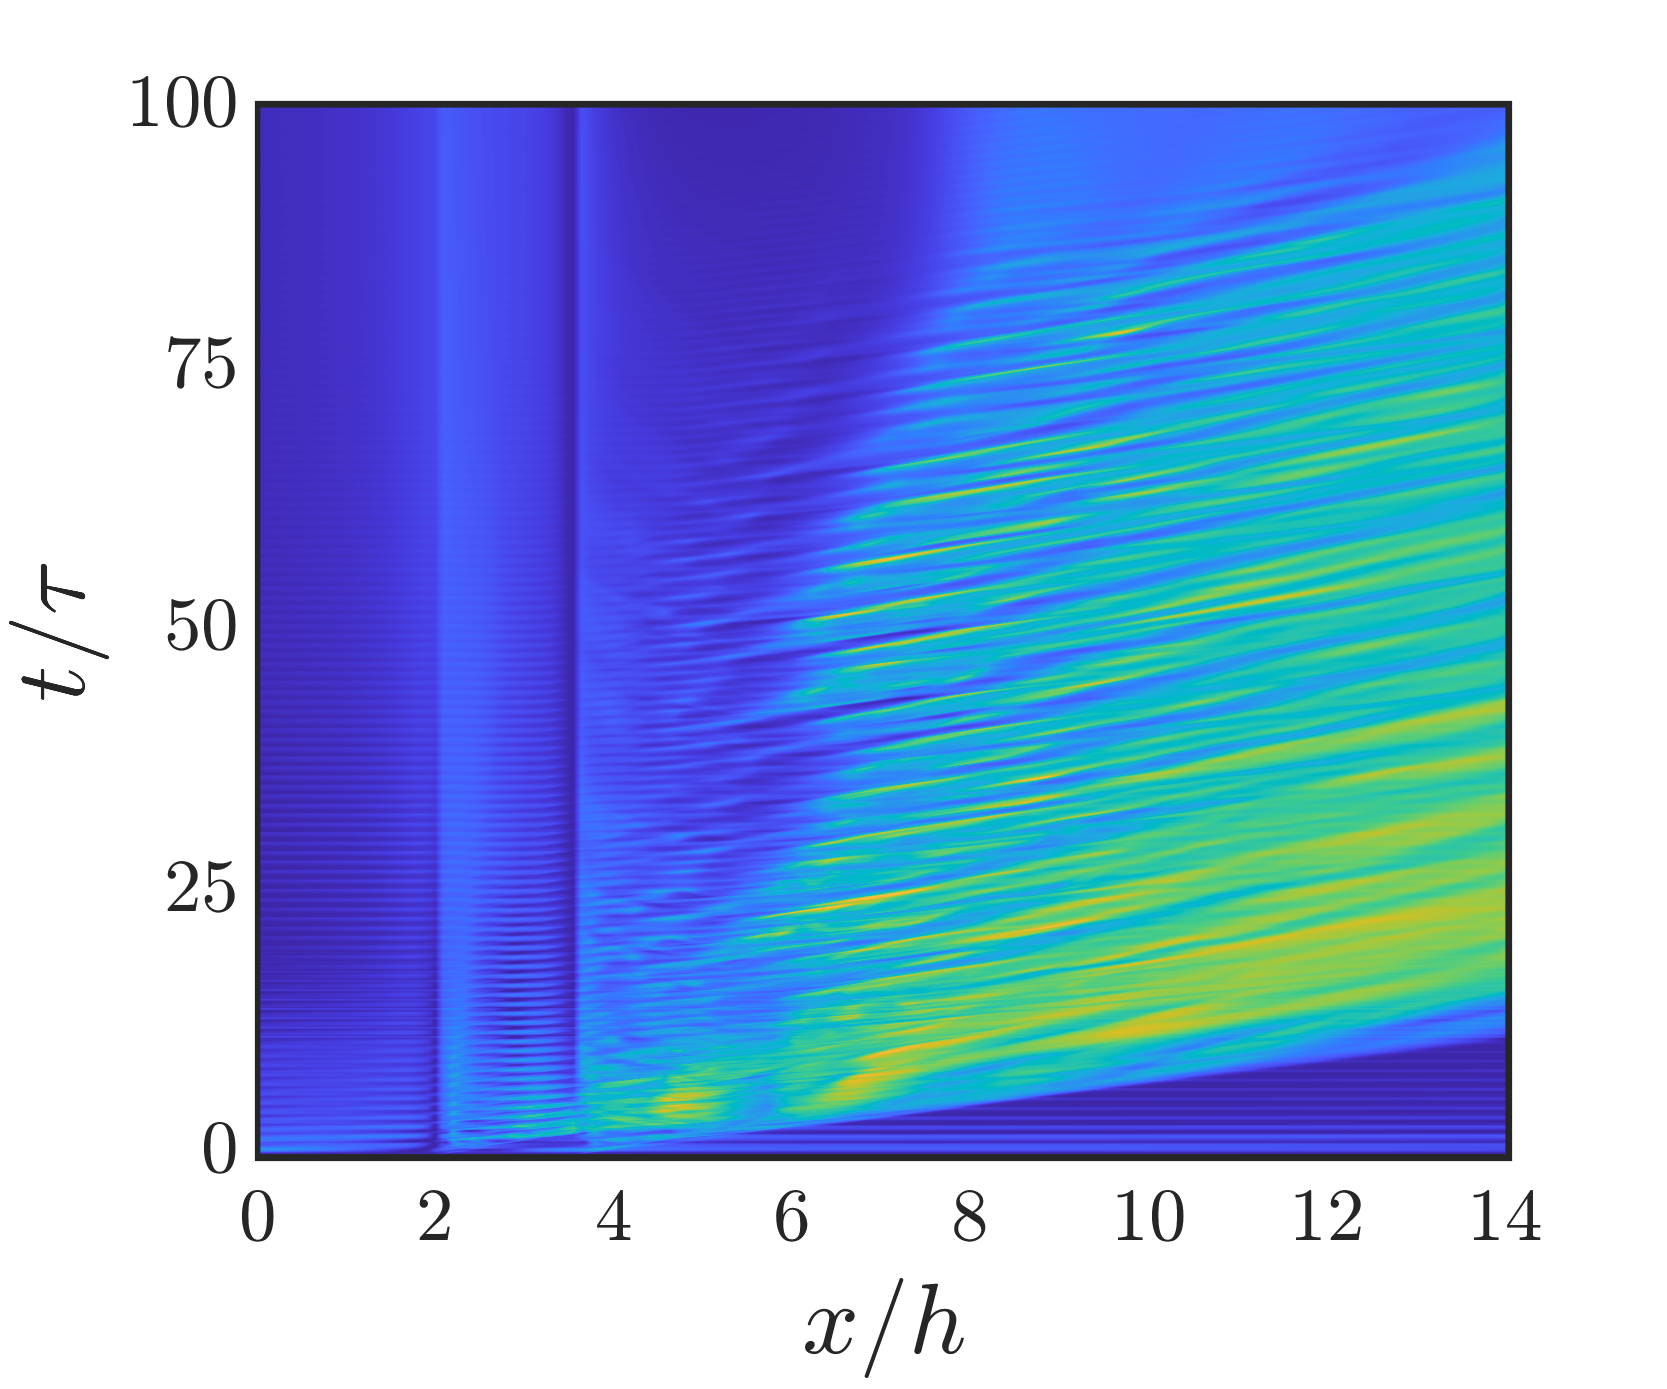
\includegraphics[width=1\linewidth]{Figures/MI_HL/spcaeTime_M_3a.png}
				%		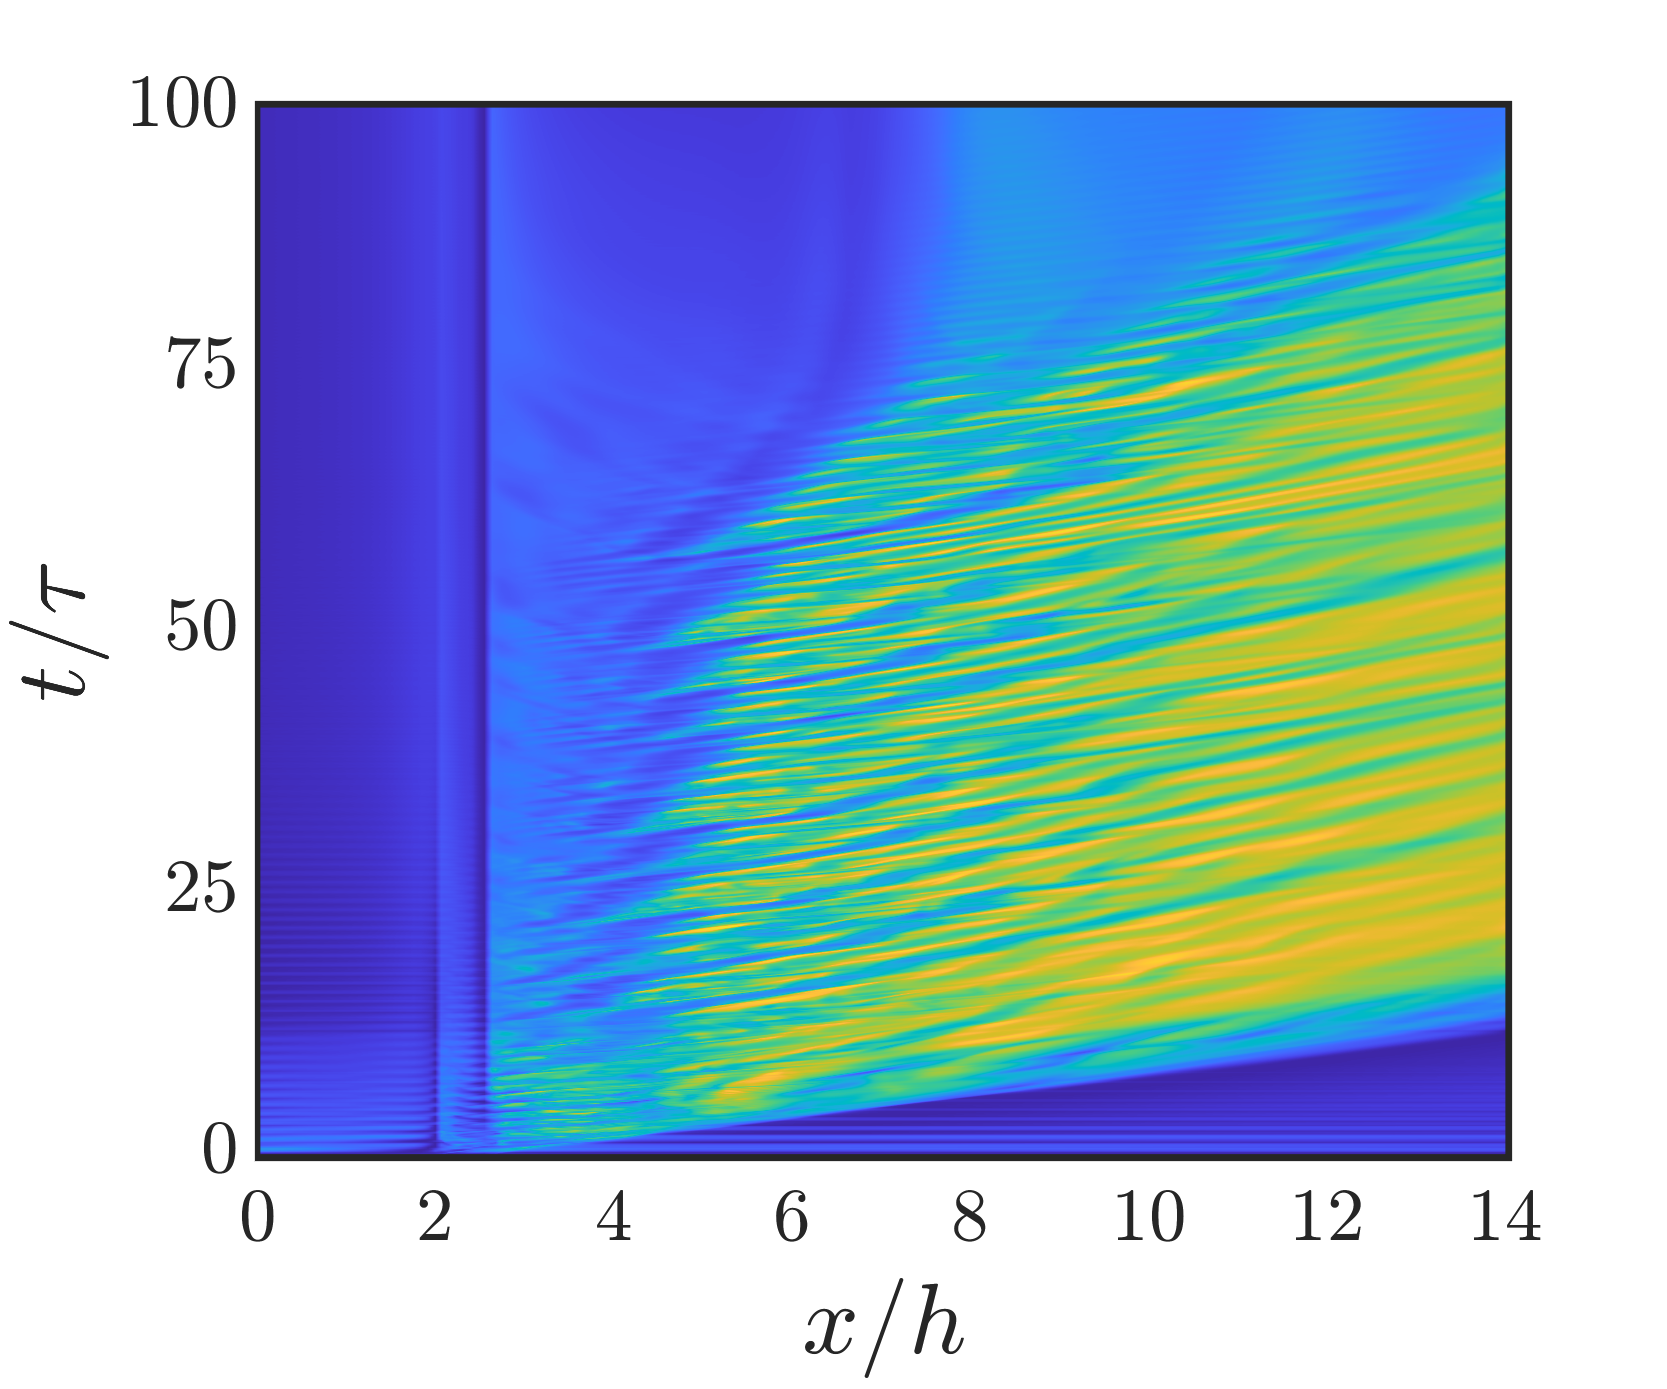
\includegraphics[width=1\linewidth]{Figures/MI_HL/spcaeTime_M_1a.png}
				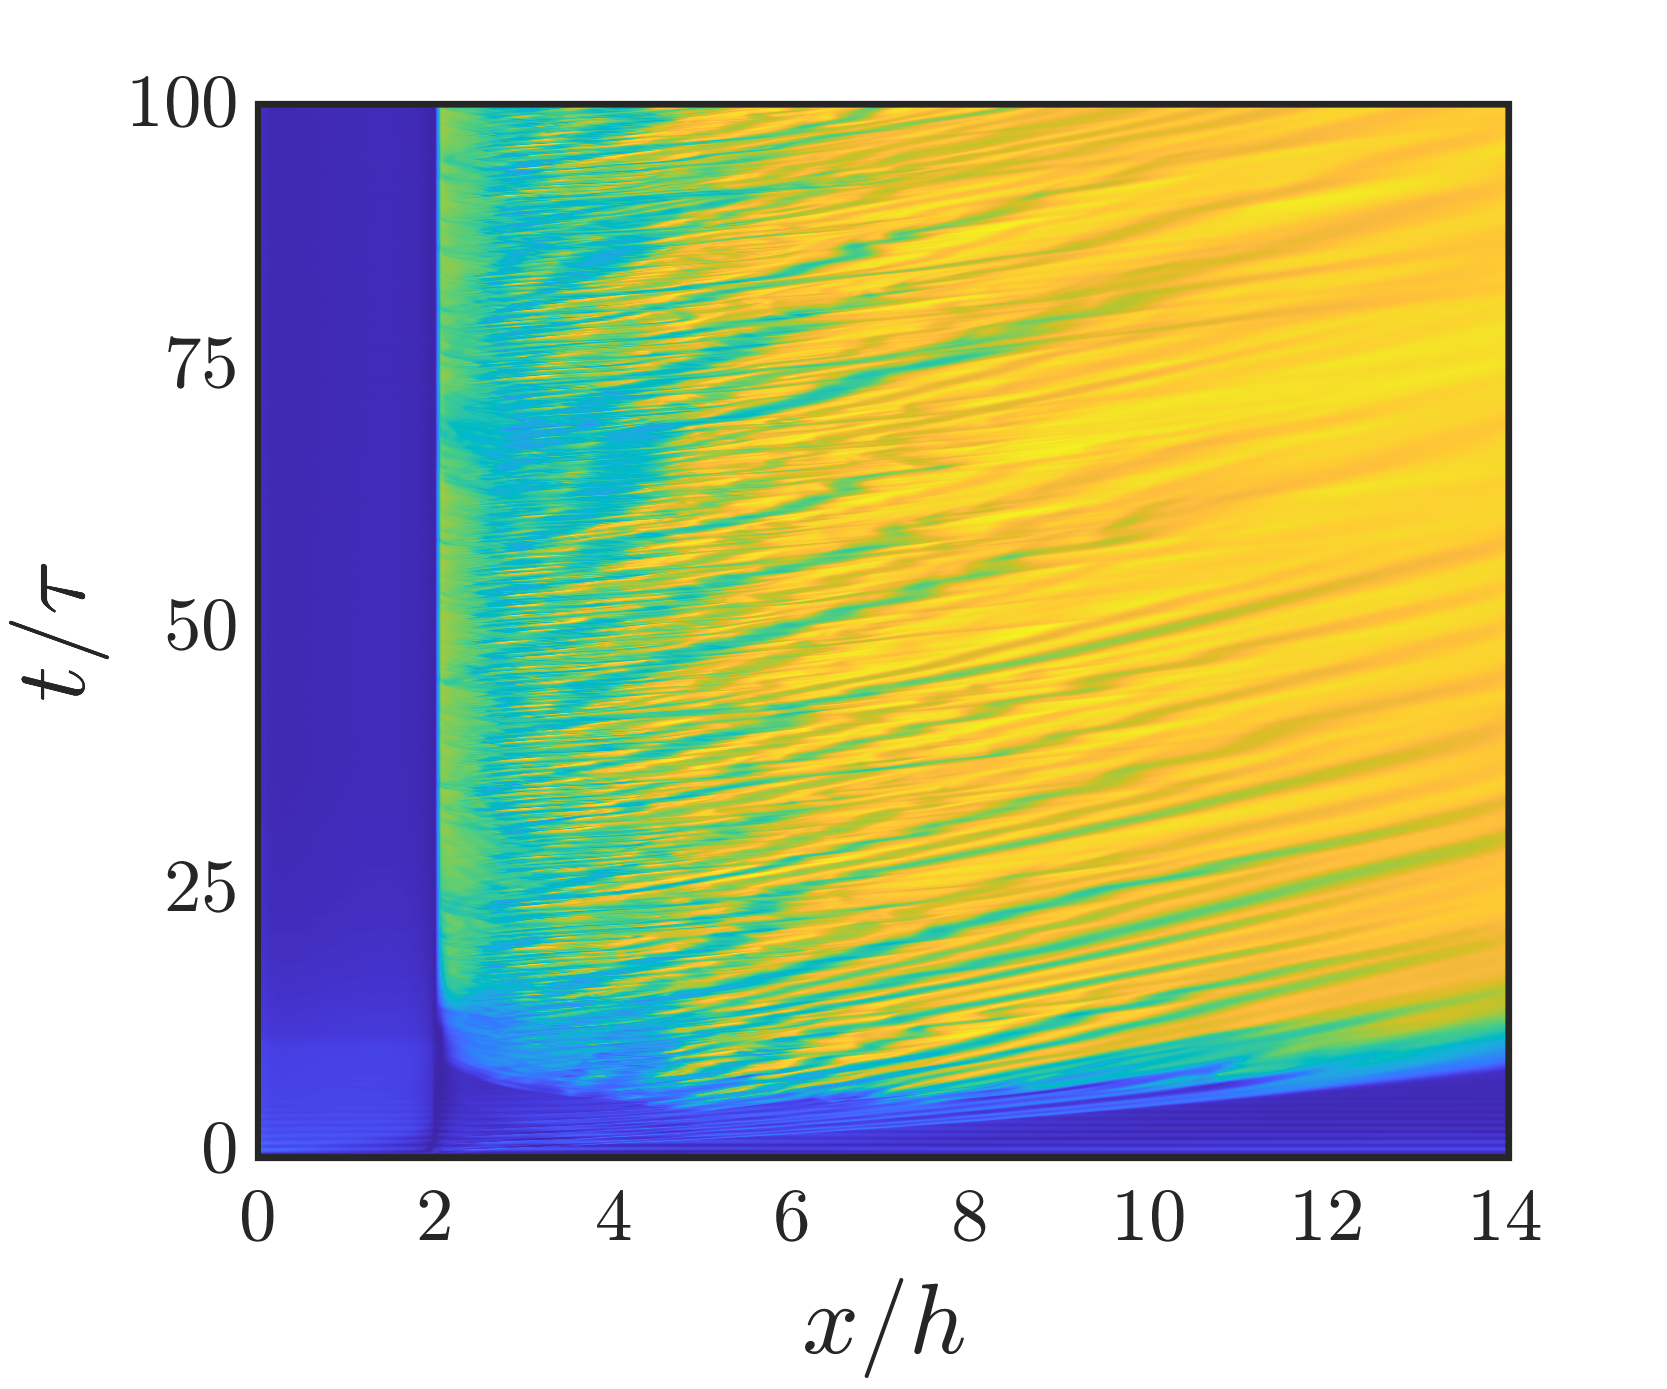
\includegraphics[width=1\linewidth,trim={1.6cm 2cm 2cm 1cm},clip]{Figures/MI_HL/spcaeTime_M_0a.png}
			\end{minipage}
			\begin{minipage}[c]{0.24\linewidth}
				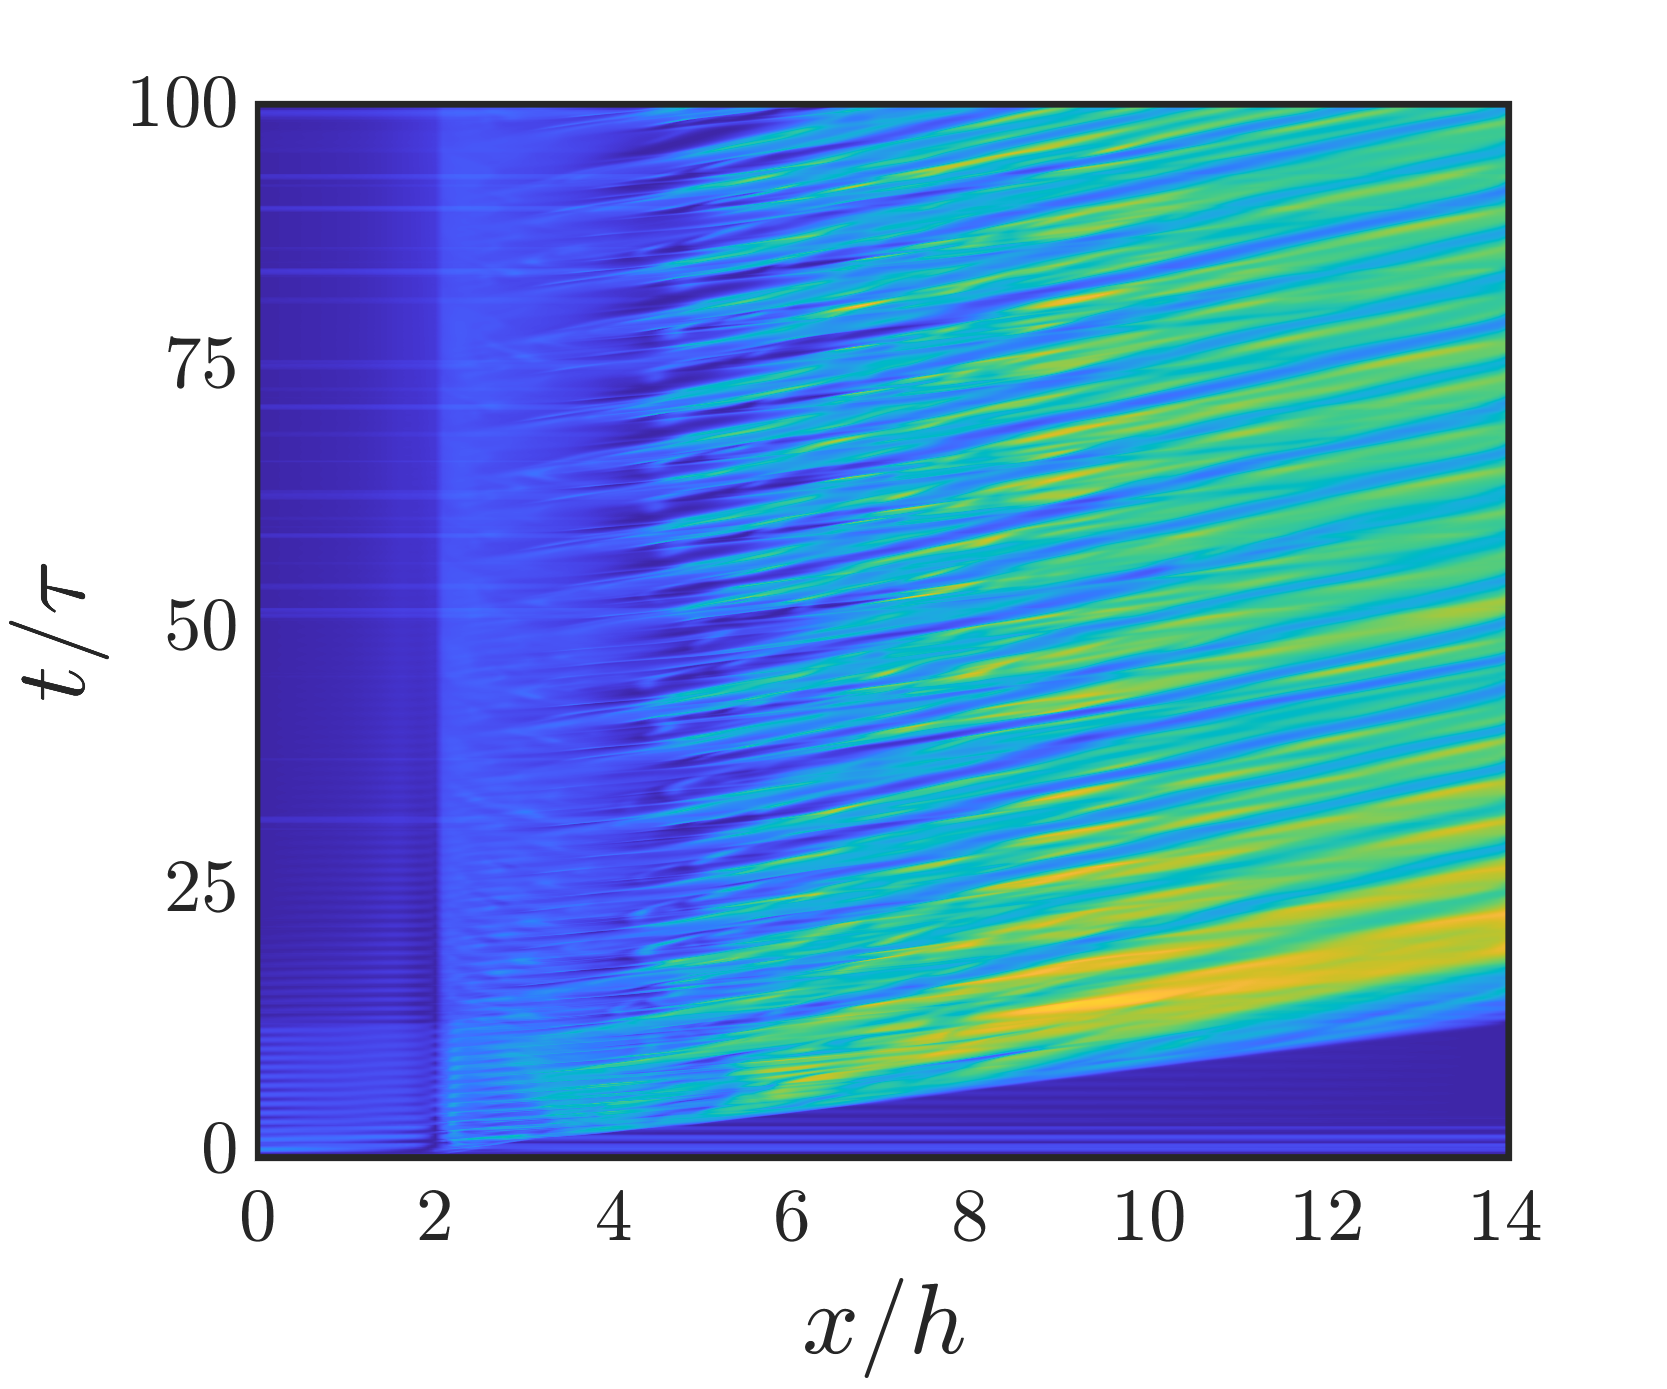
\includegraphics[width=1\linewidth,trim={1.6cm 2cm 2cm 1cm},clip]{Figures/MI_HL/spcaeTime_M_Singleb.png}
				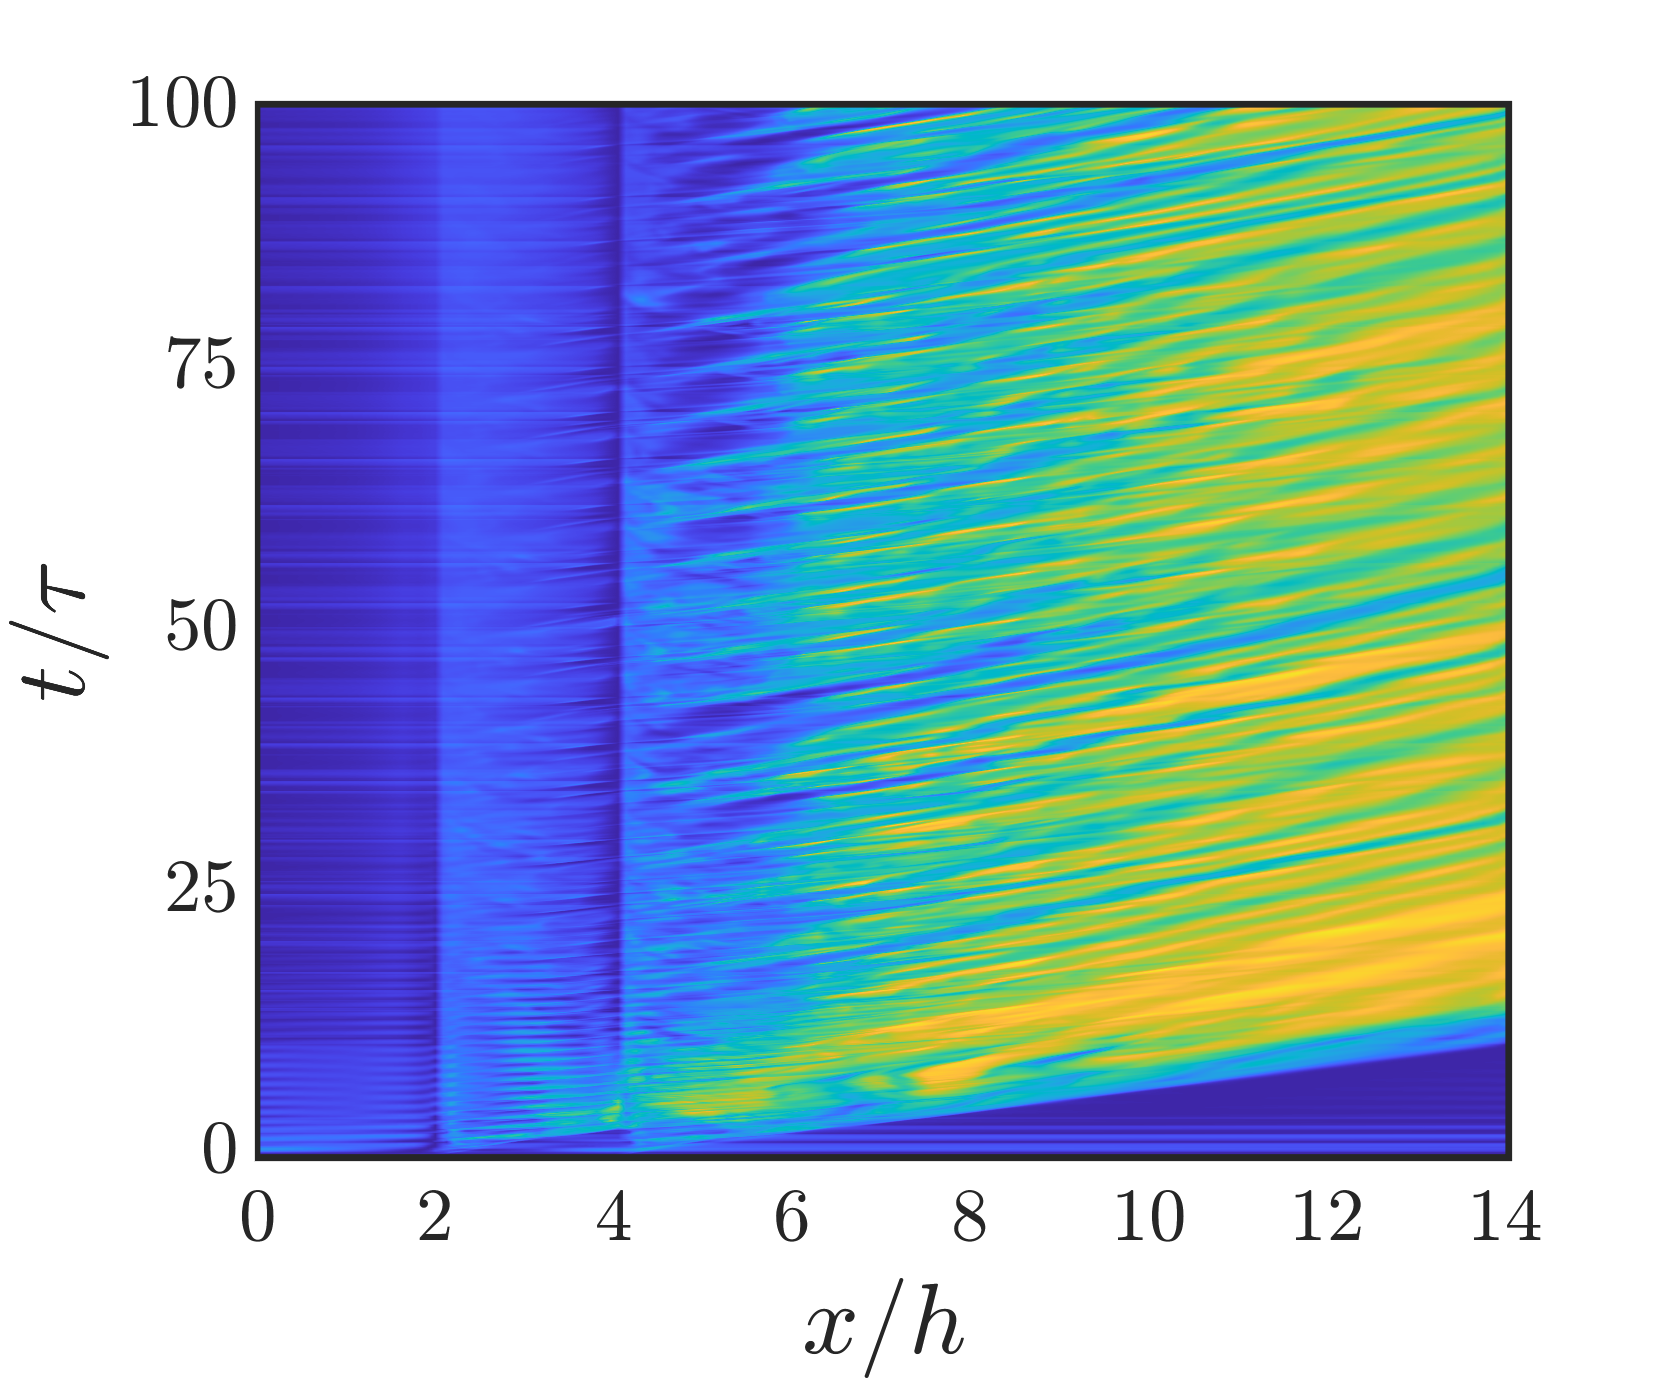
\includegraphics[width=1\linewidth,trim={1.6cm 2cm 2cm 1cm},clip]{Figures/MI_HL/spcaeTime_M_4b.png}
				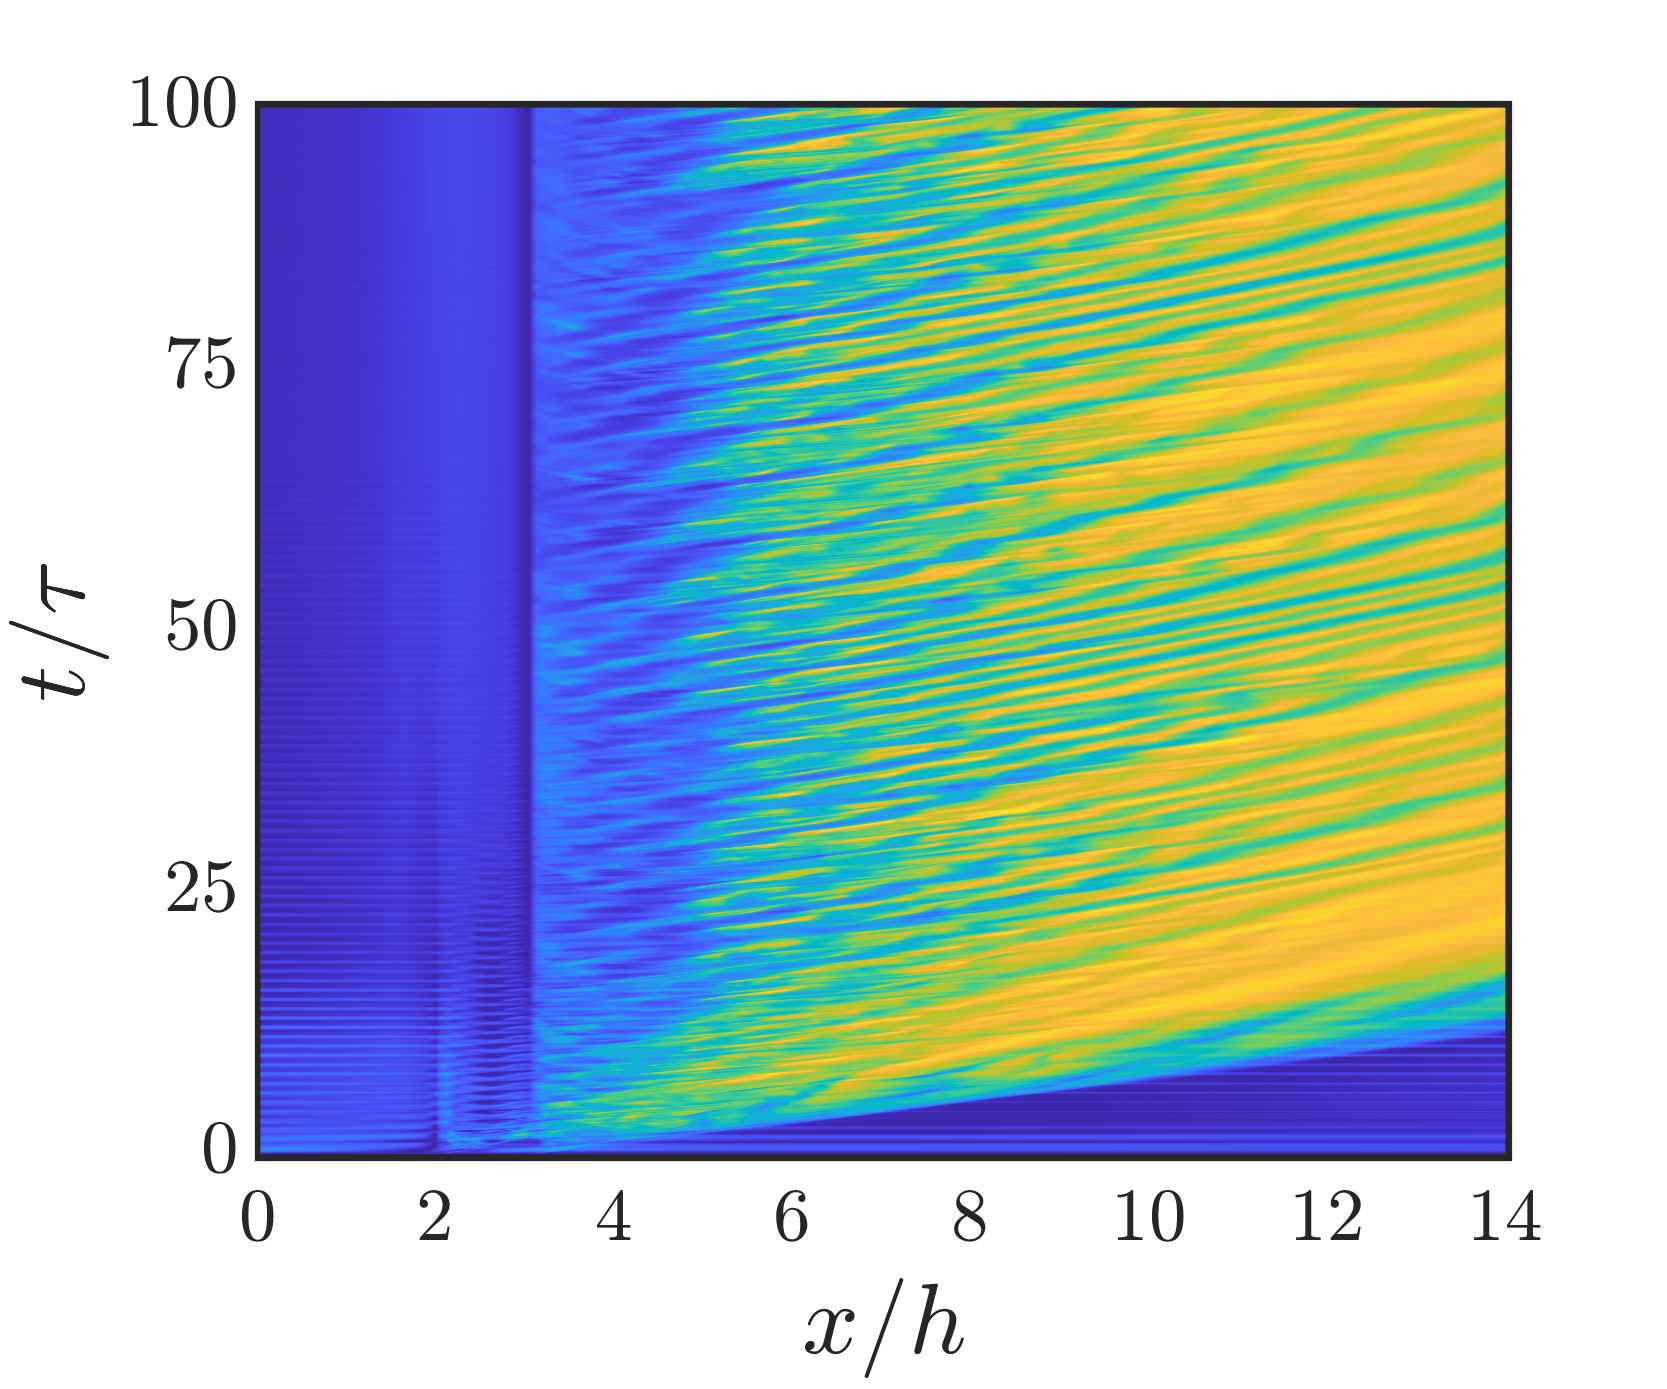
\includegraphics[width=1\linewidth,trim={1.6cm 2cm 2cm 1cm},clip]{Figures/MI_HL/spcaeTime_M_2b.png}
				%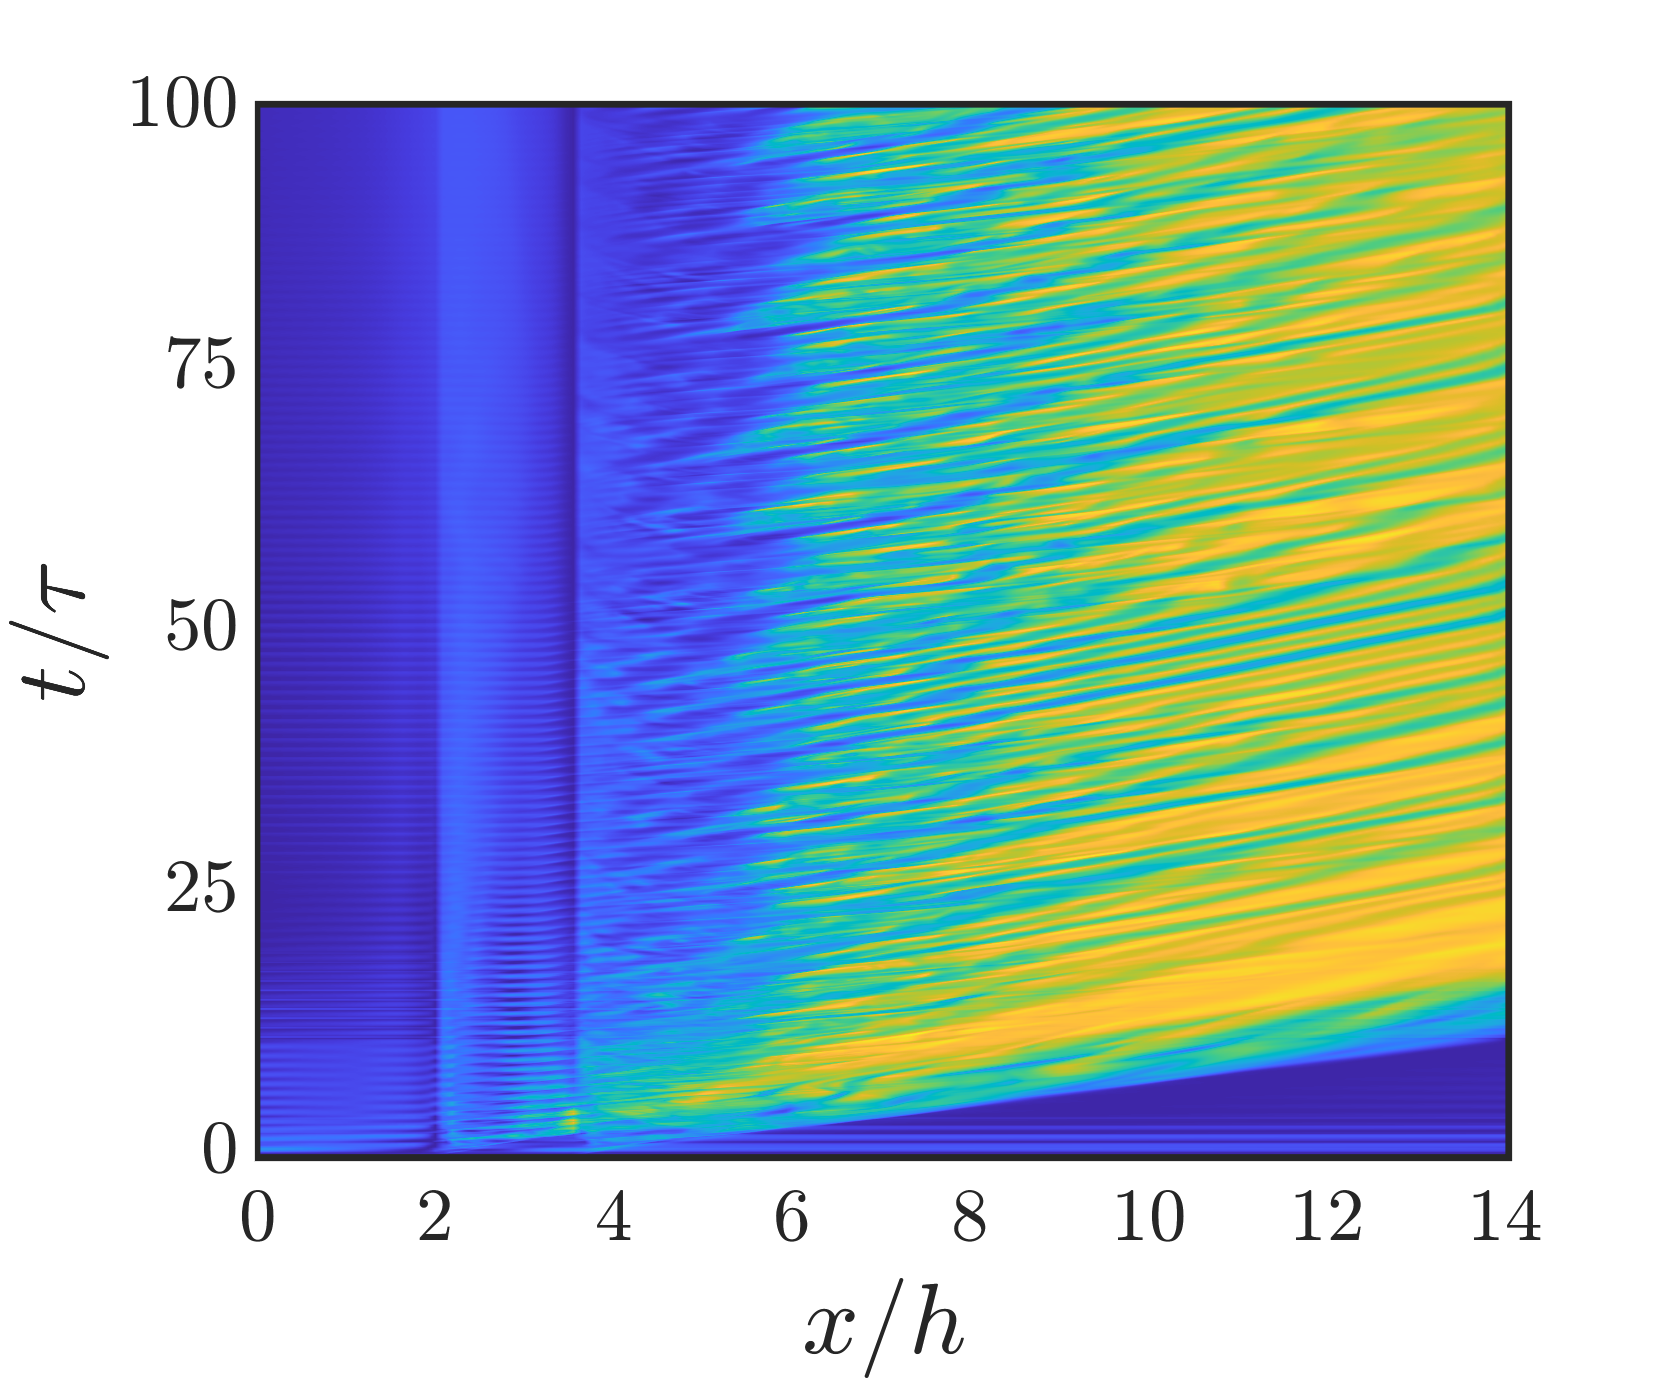
\includegraphics[width=1\linewidth]{Figures/MI_HL/spcaeTime_M_3b.png}
				%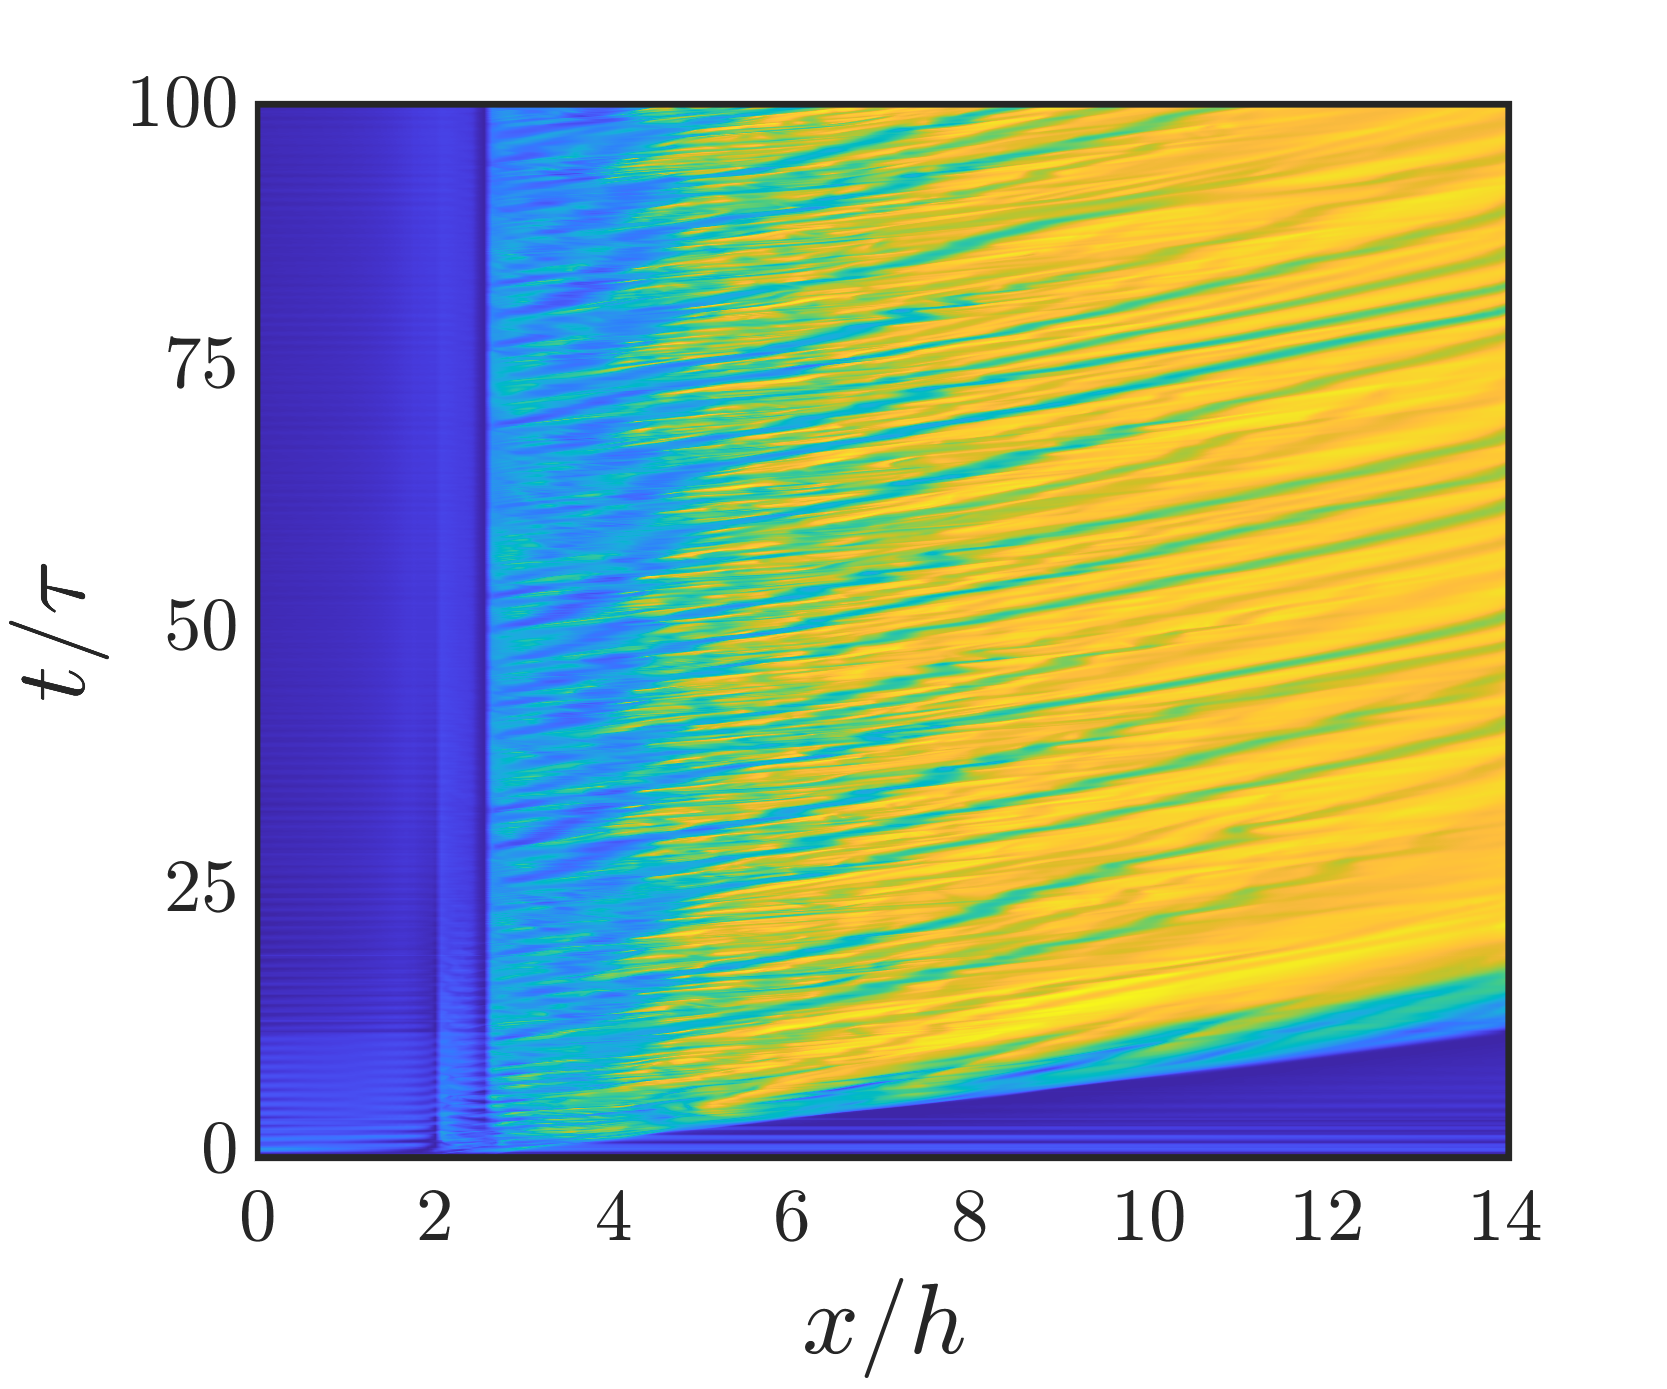
\includegraphics[width=1\linewidth]{Figures/MI_HL/spcaeTime_M_1b.png}
				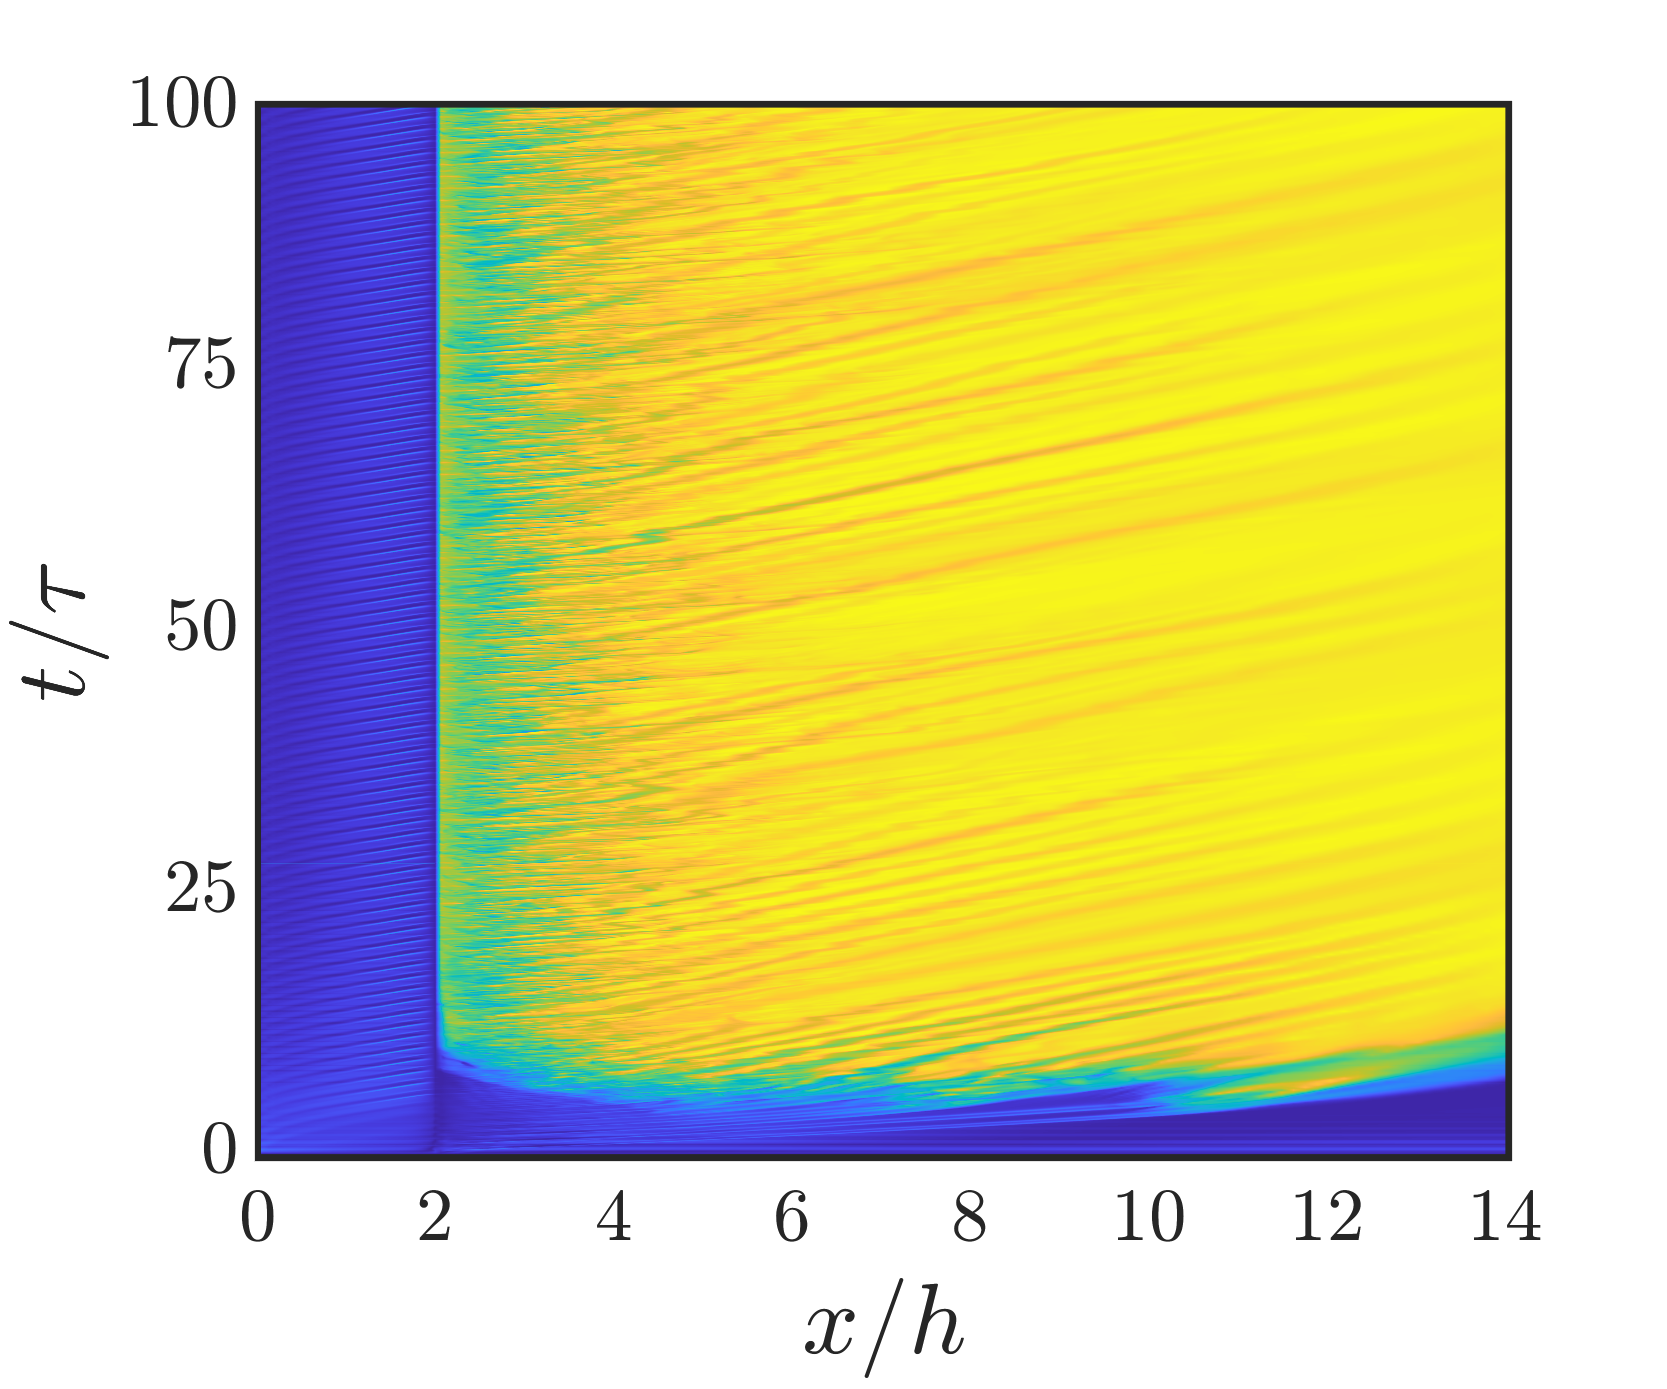
\includegraphics[width=1\linewidth,trim={1.6cm 2cm 2cm 1cm},clip]{Figures/MI_HL/spcaeTime_M_0b.png}
			\end{minipage}
			\begin{minipage}[c]{0.24\linewidth}
				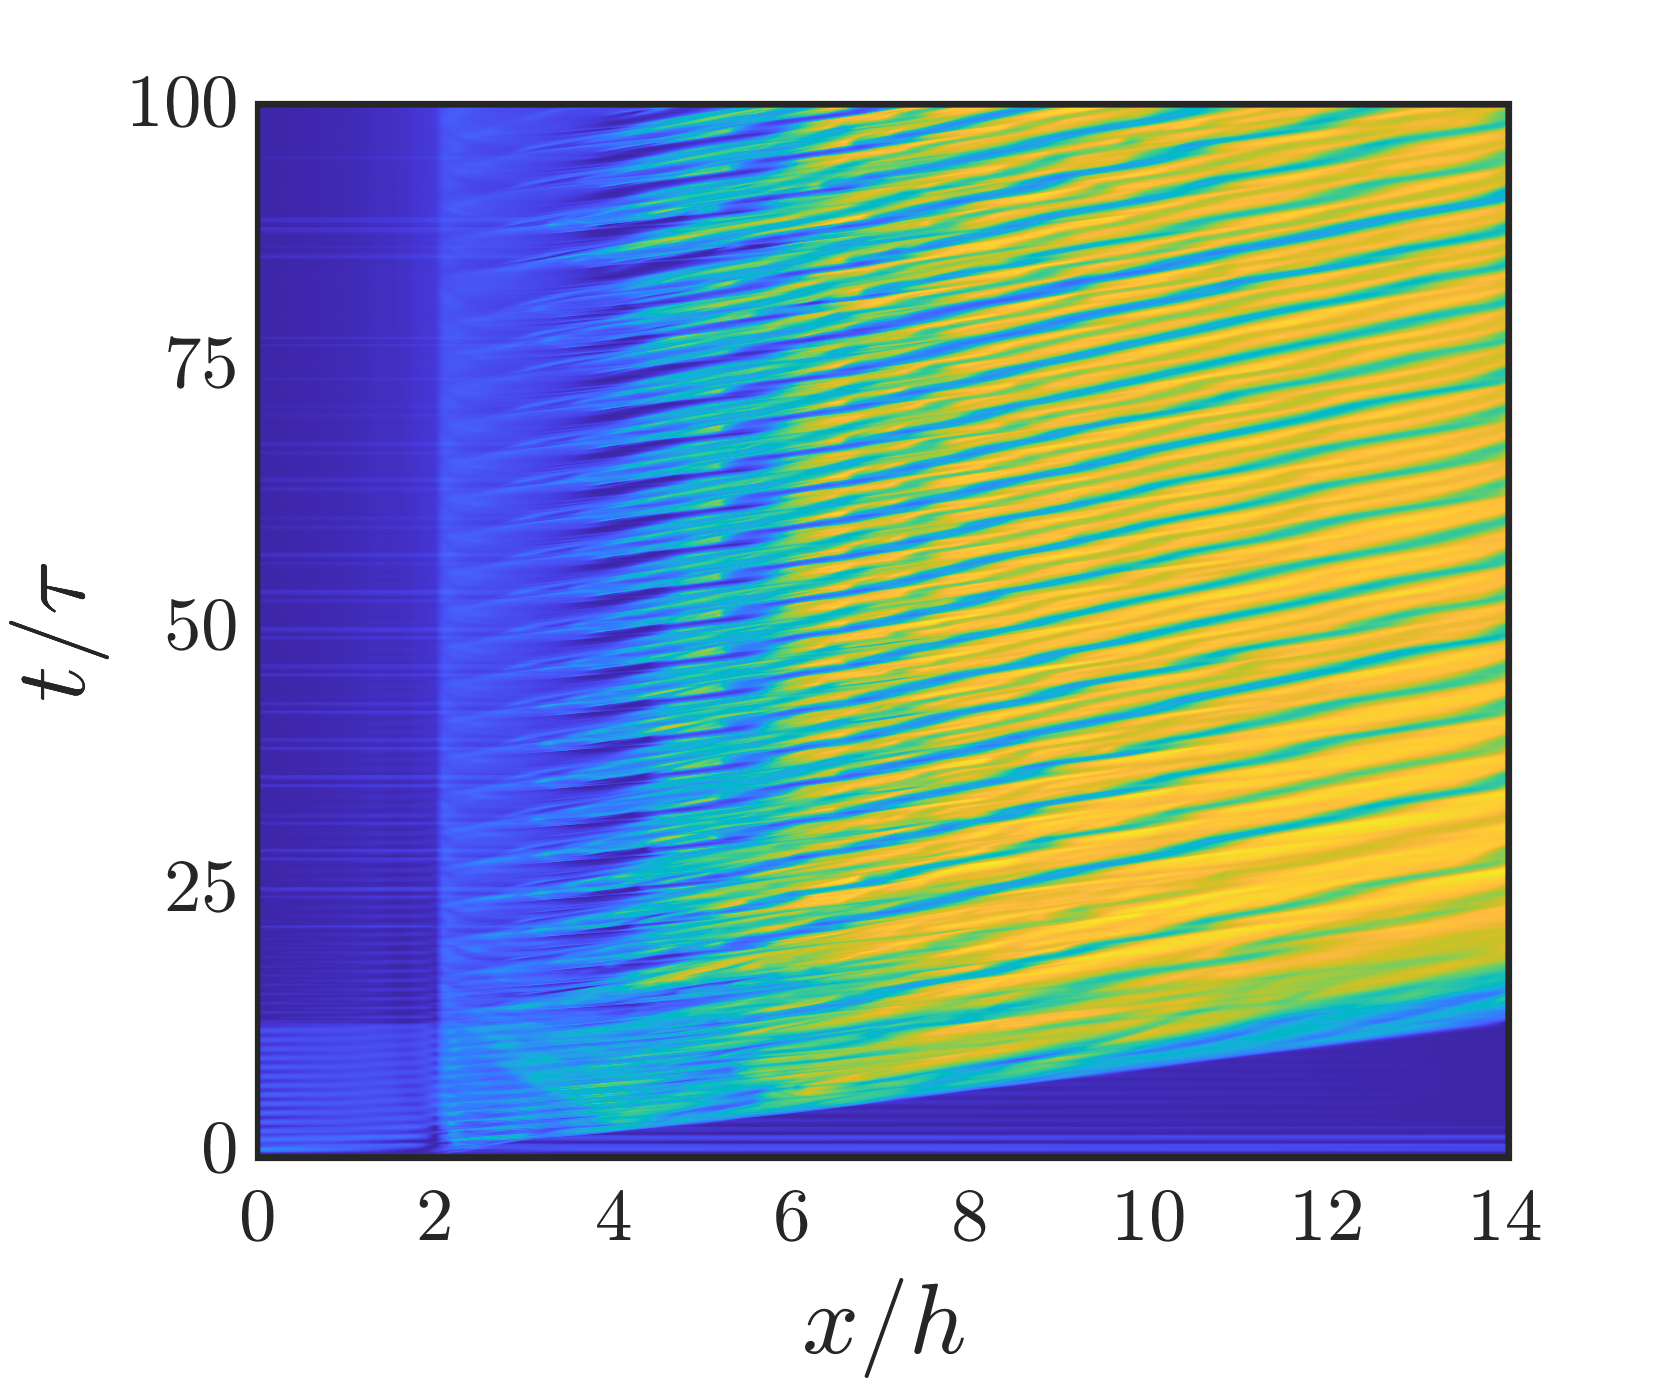
\includegraphics[width=1\linewidth,trim={1.6cm 2cm 2cm 1cm},clip]{Figures/MI_HL/spcaeTime_M_Singlec.png}
				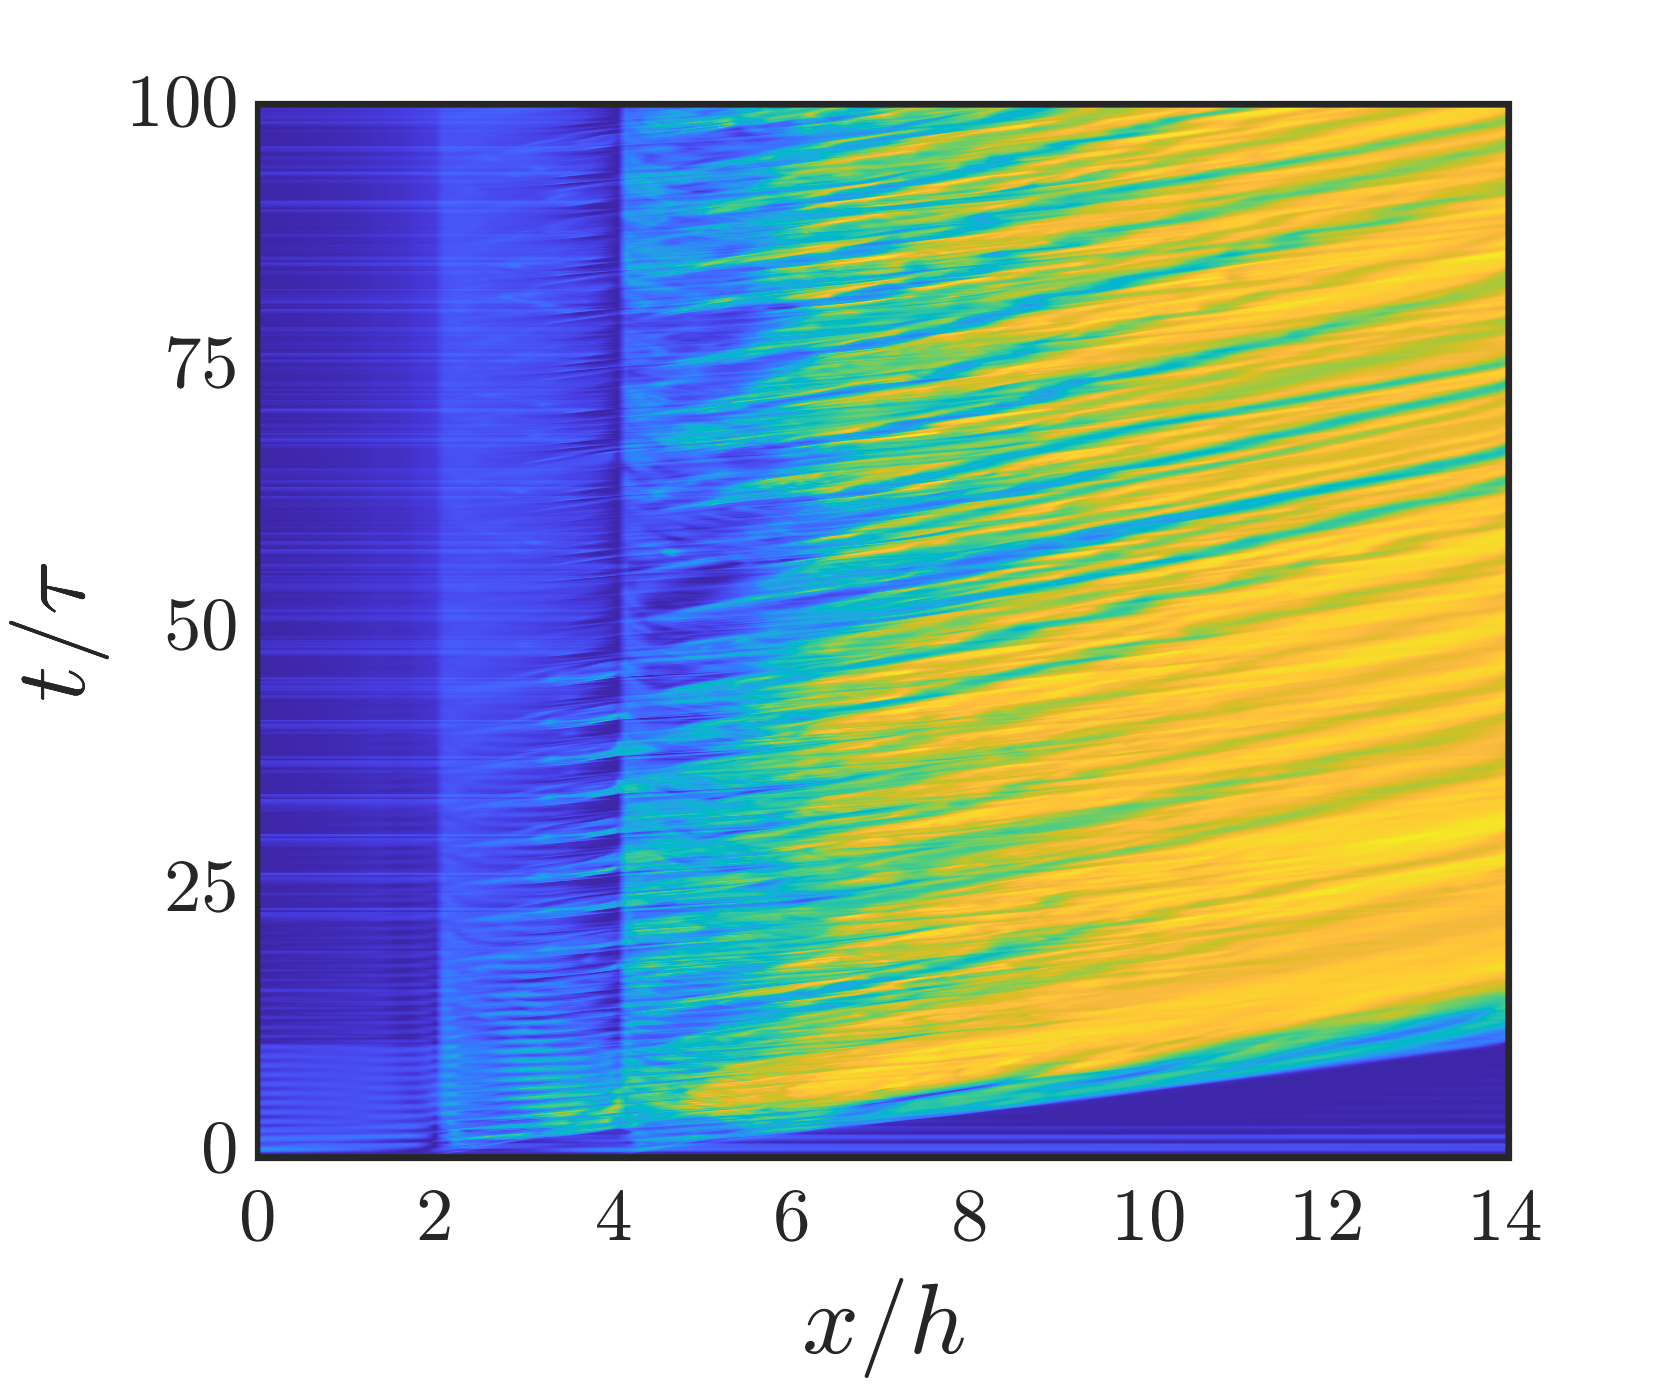
\includegraphics[width=1\linewidth,trim={1.6cm 2cm 2cm 1cm},clip]{Figures/MI_HL/spcaeTime_M_4c.png}
				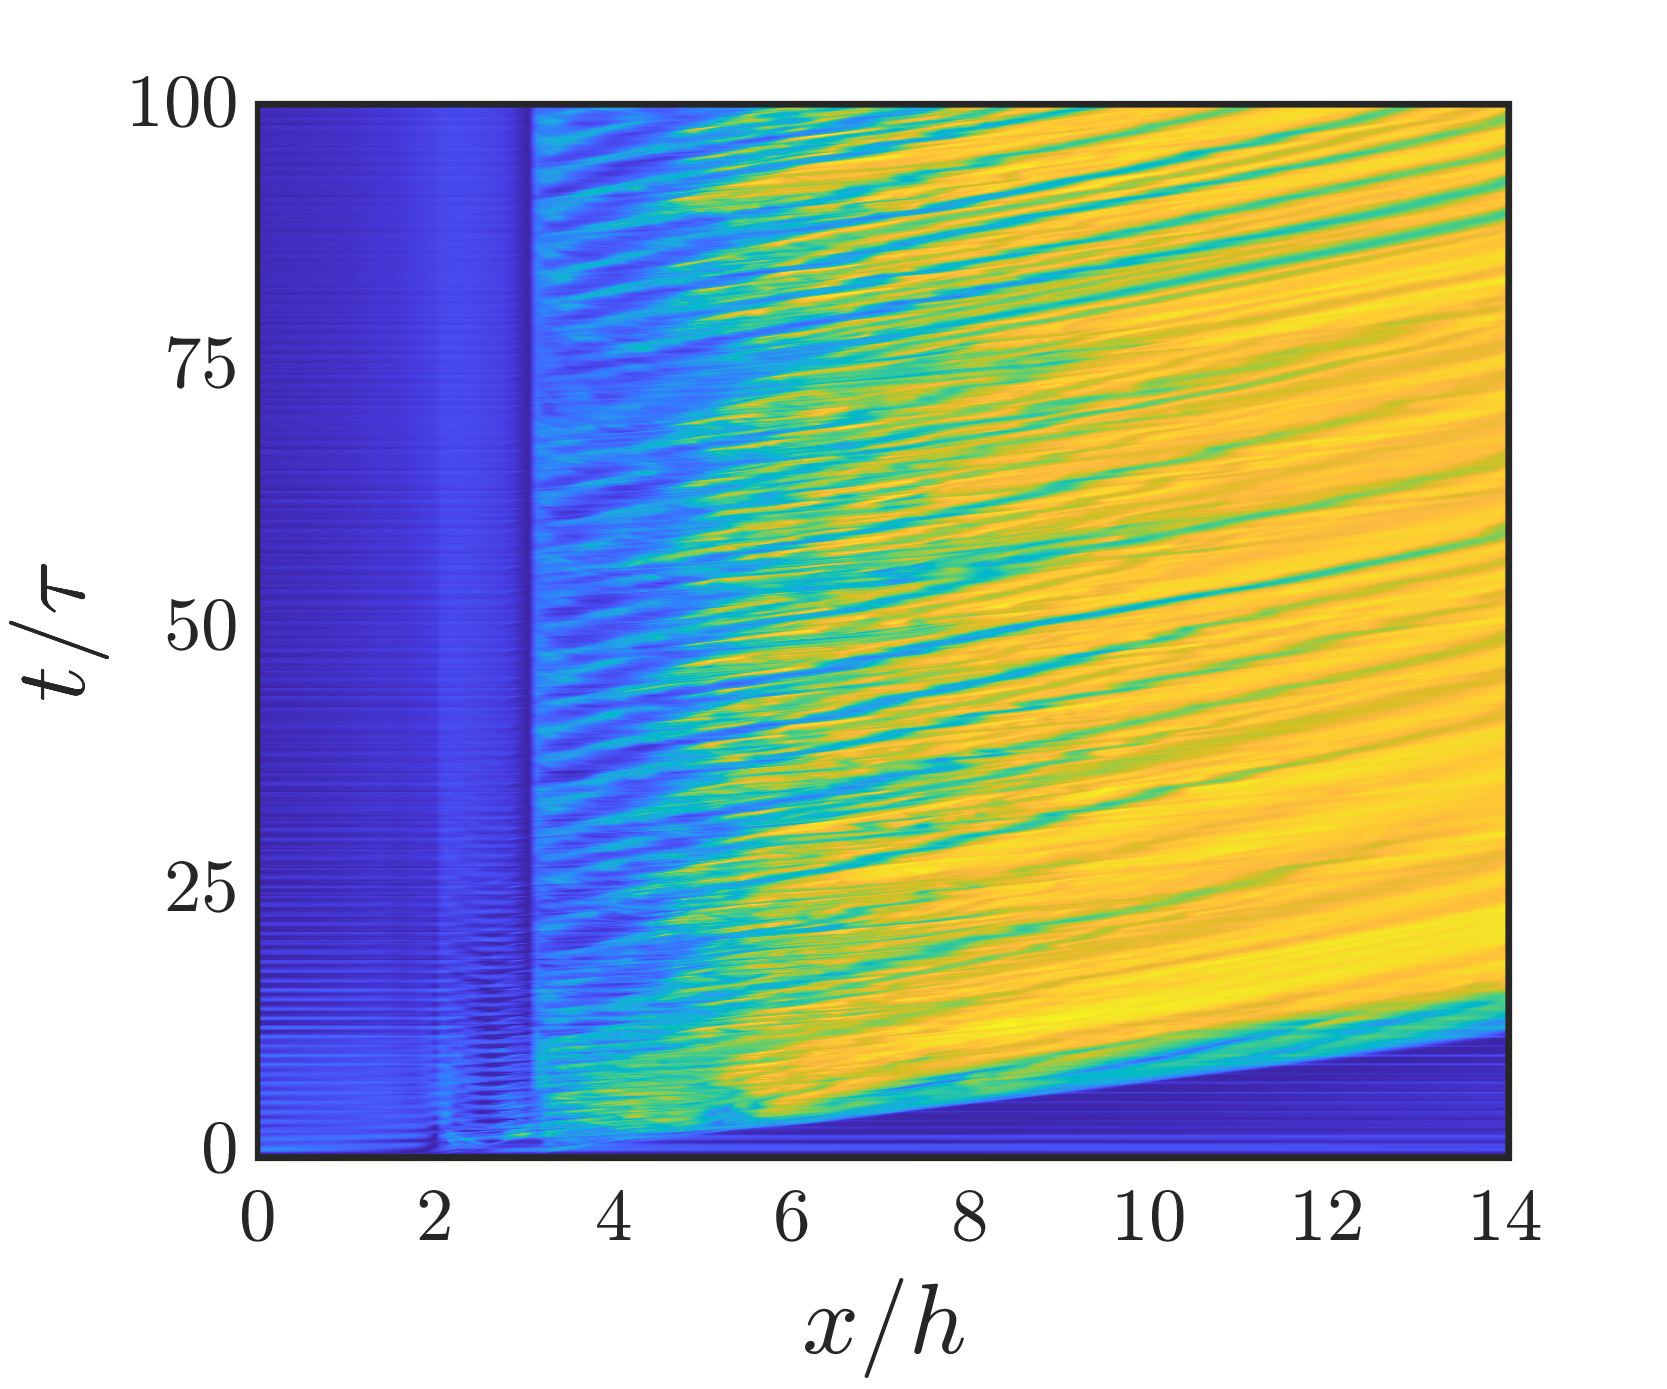
\includegraphics[width=1\linewidth,trim={1.6cm 2cm 2cm 1cm},clip]{Figures/MI_HL/spcaeTime_M_2c.png}
				%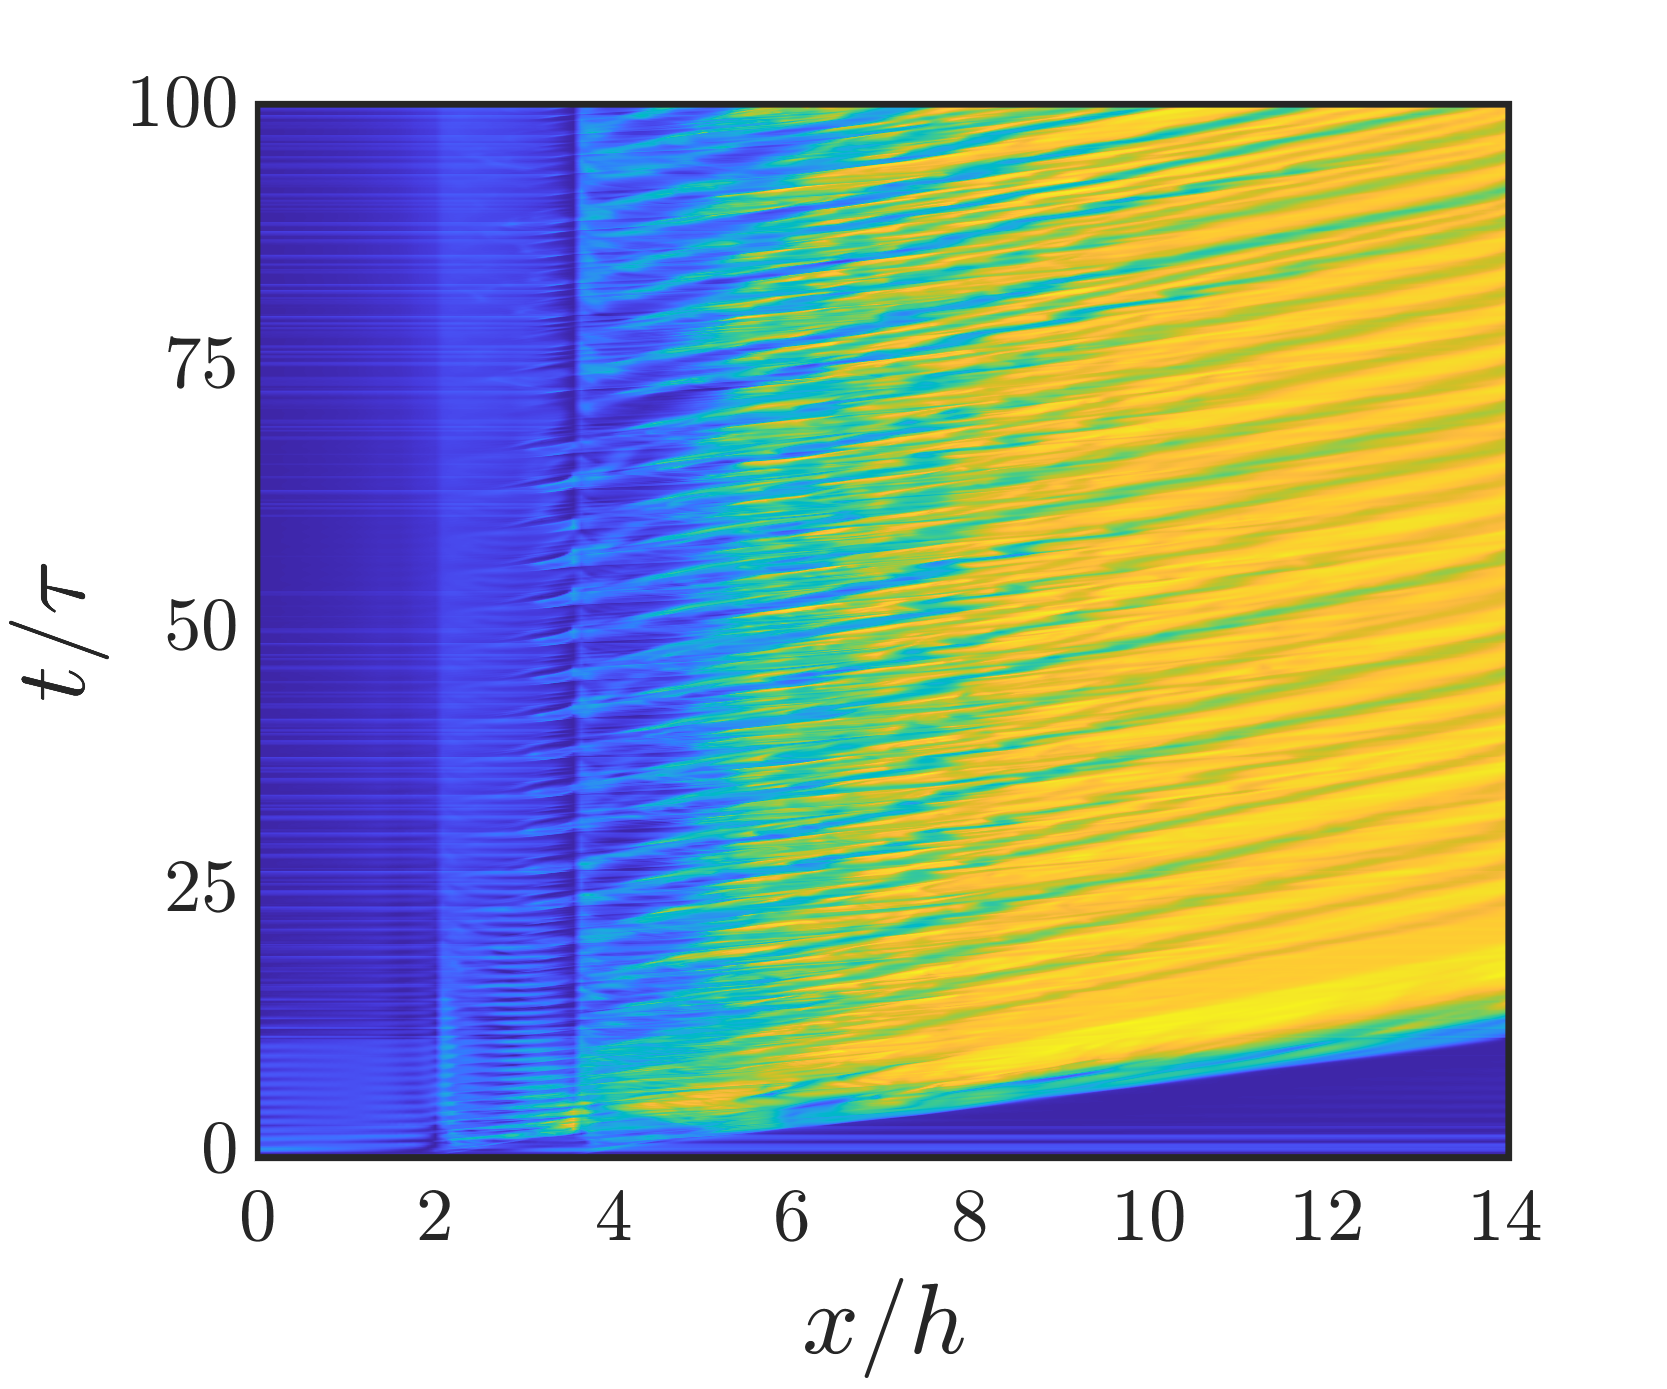
\includegraphics[width=1\linewidth]{Figures/MI_HL/spcaeTime_M_3c.png}
				%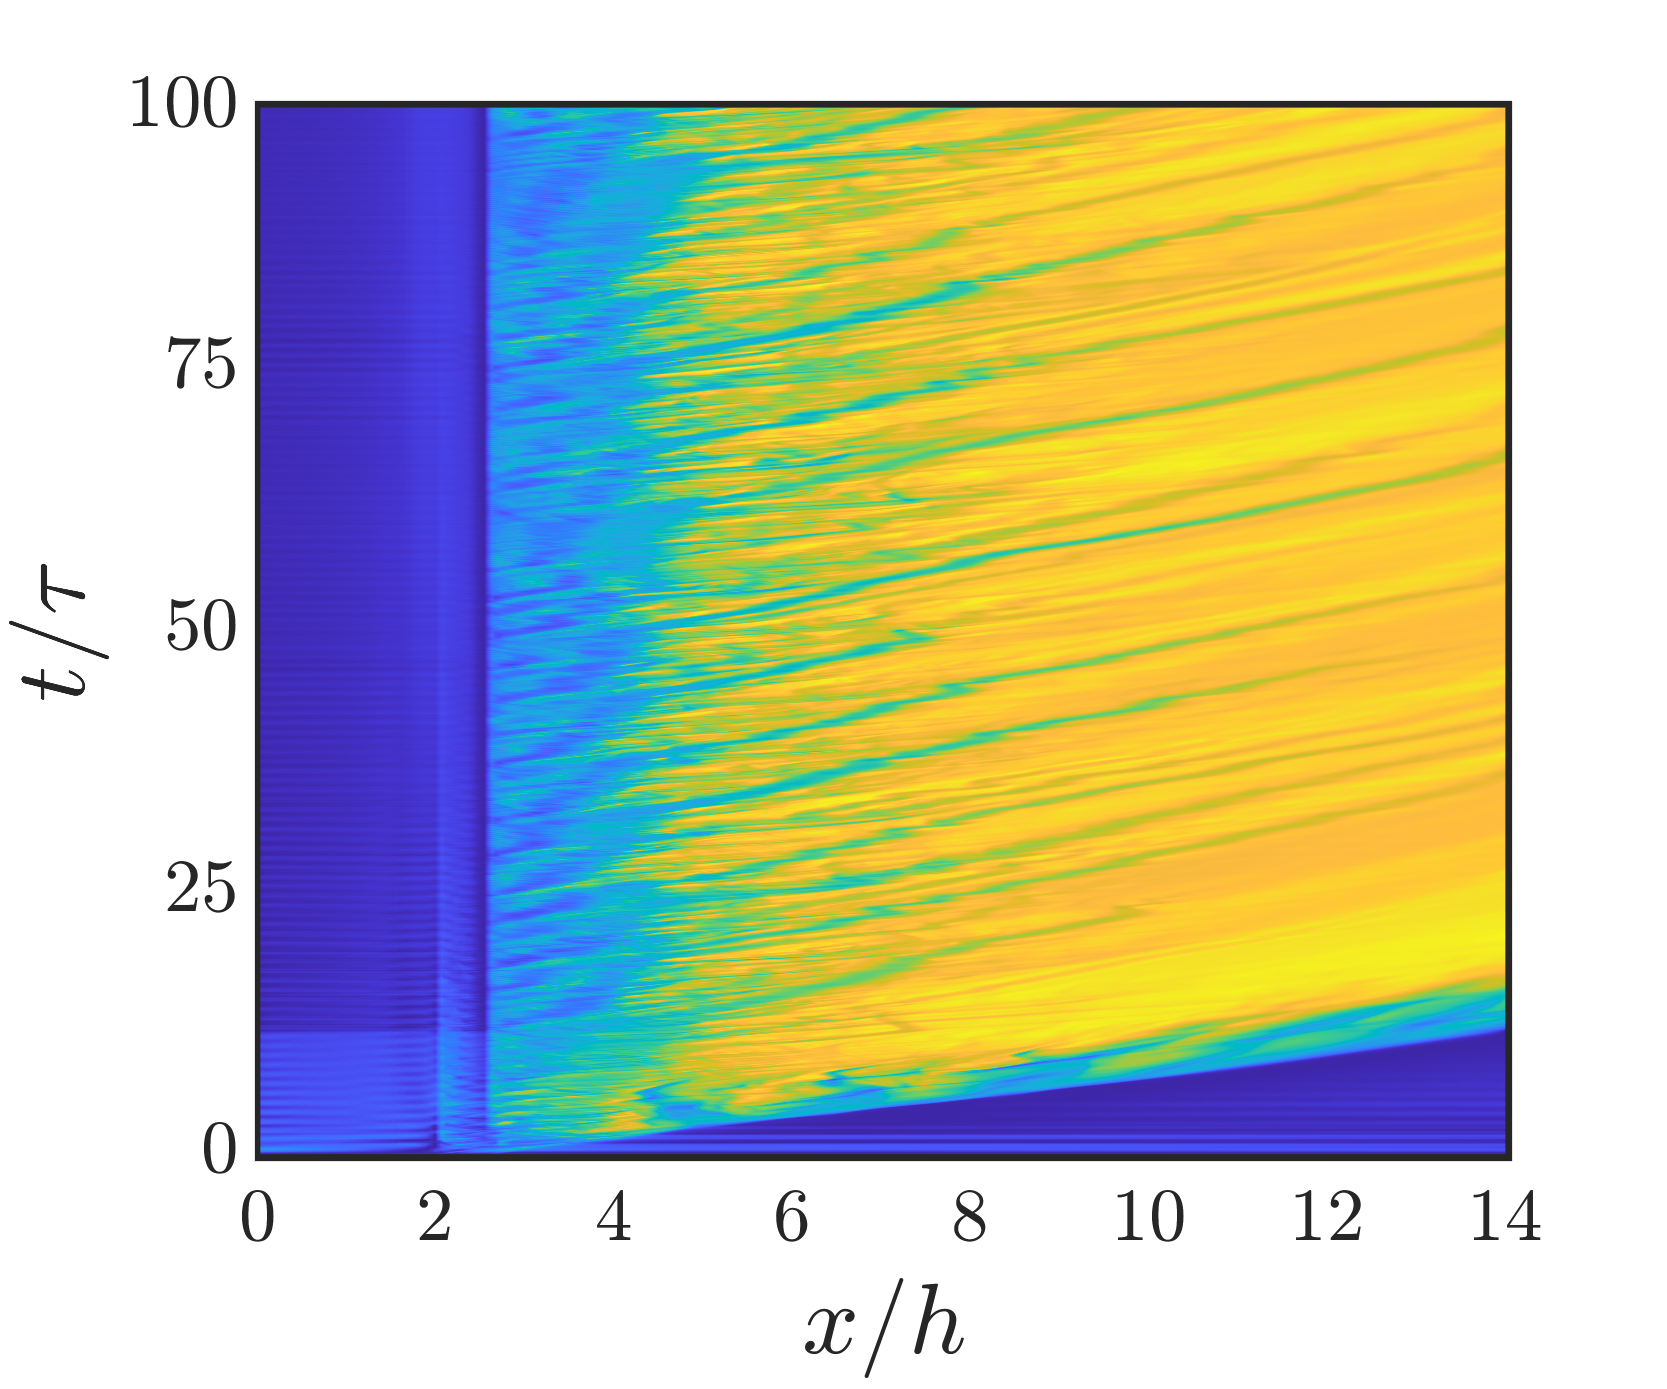
\includegraphics[width=1\linewidth]{Figures/MI_HL/spcaeTime_M_1c.png}
				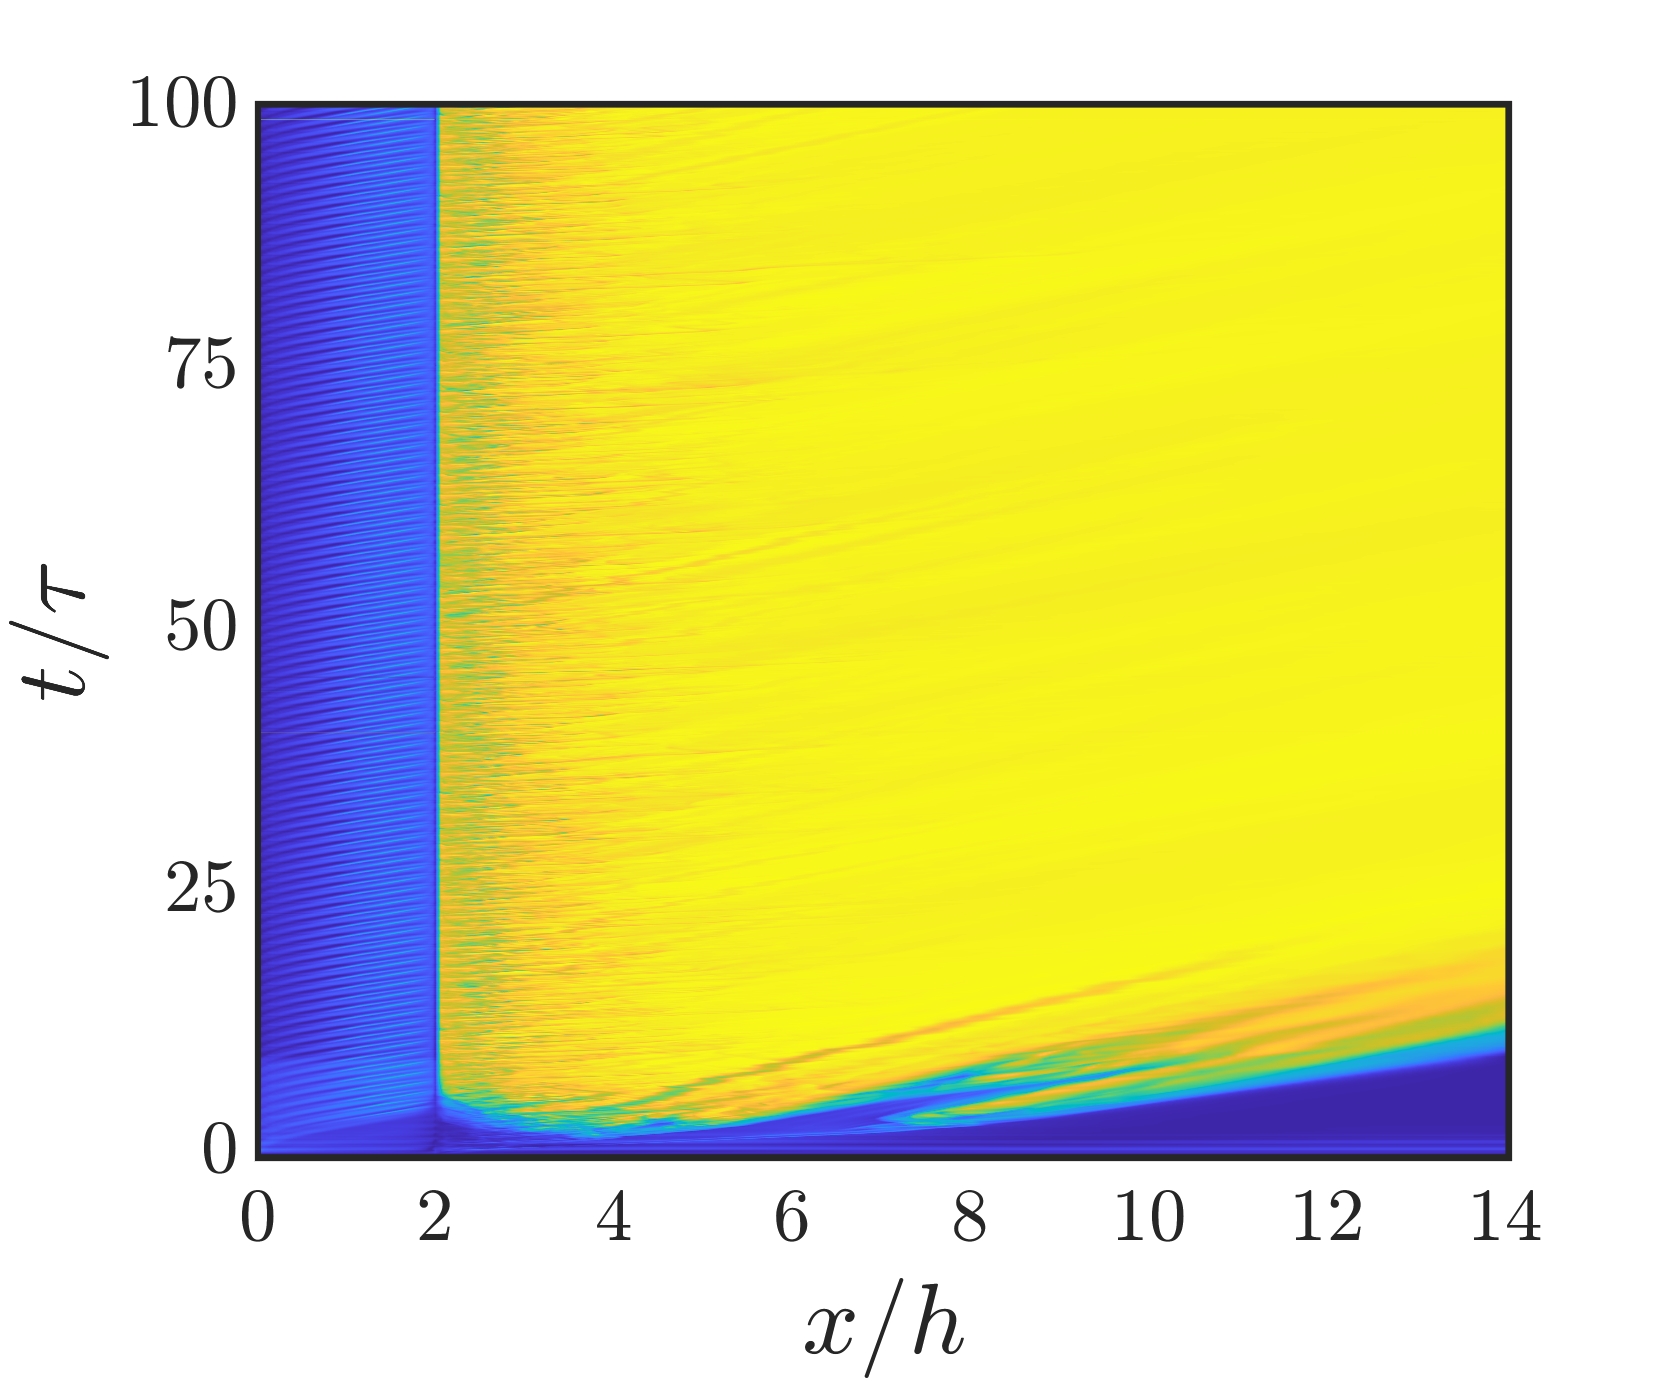
\includegraphics[width=1\linewidth,trim={1.6cm 2cm 2cm 1cm},clip]{Figures/MI_HL/spcaeTime_M_0c.png}
			\end{minipage}
			%		\begin{minipage}[c]{0.195\linewidth}
				%		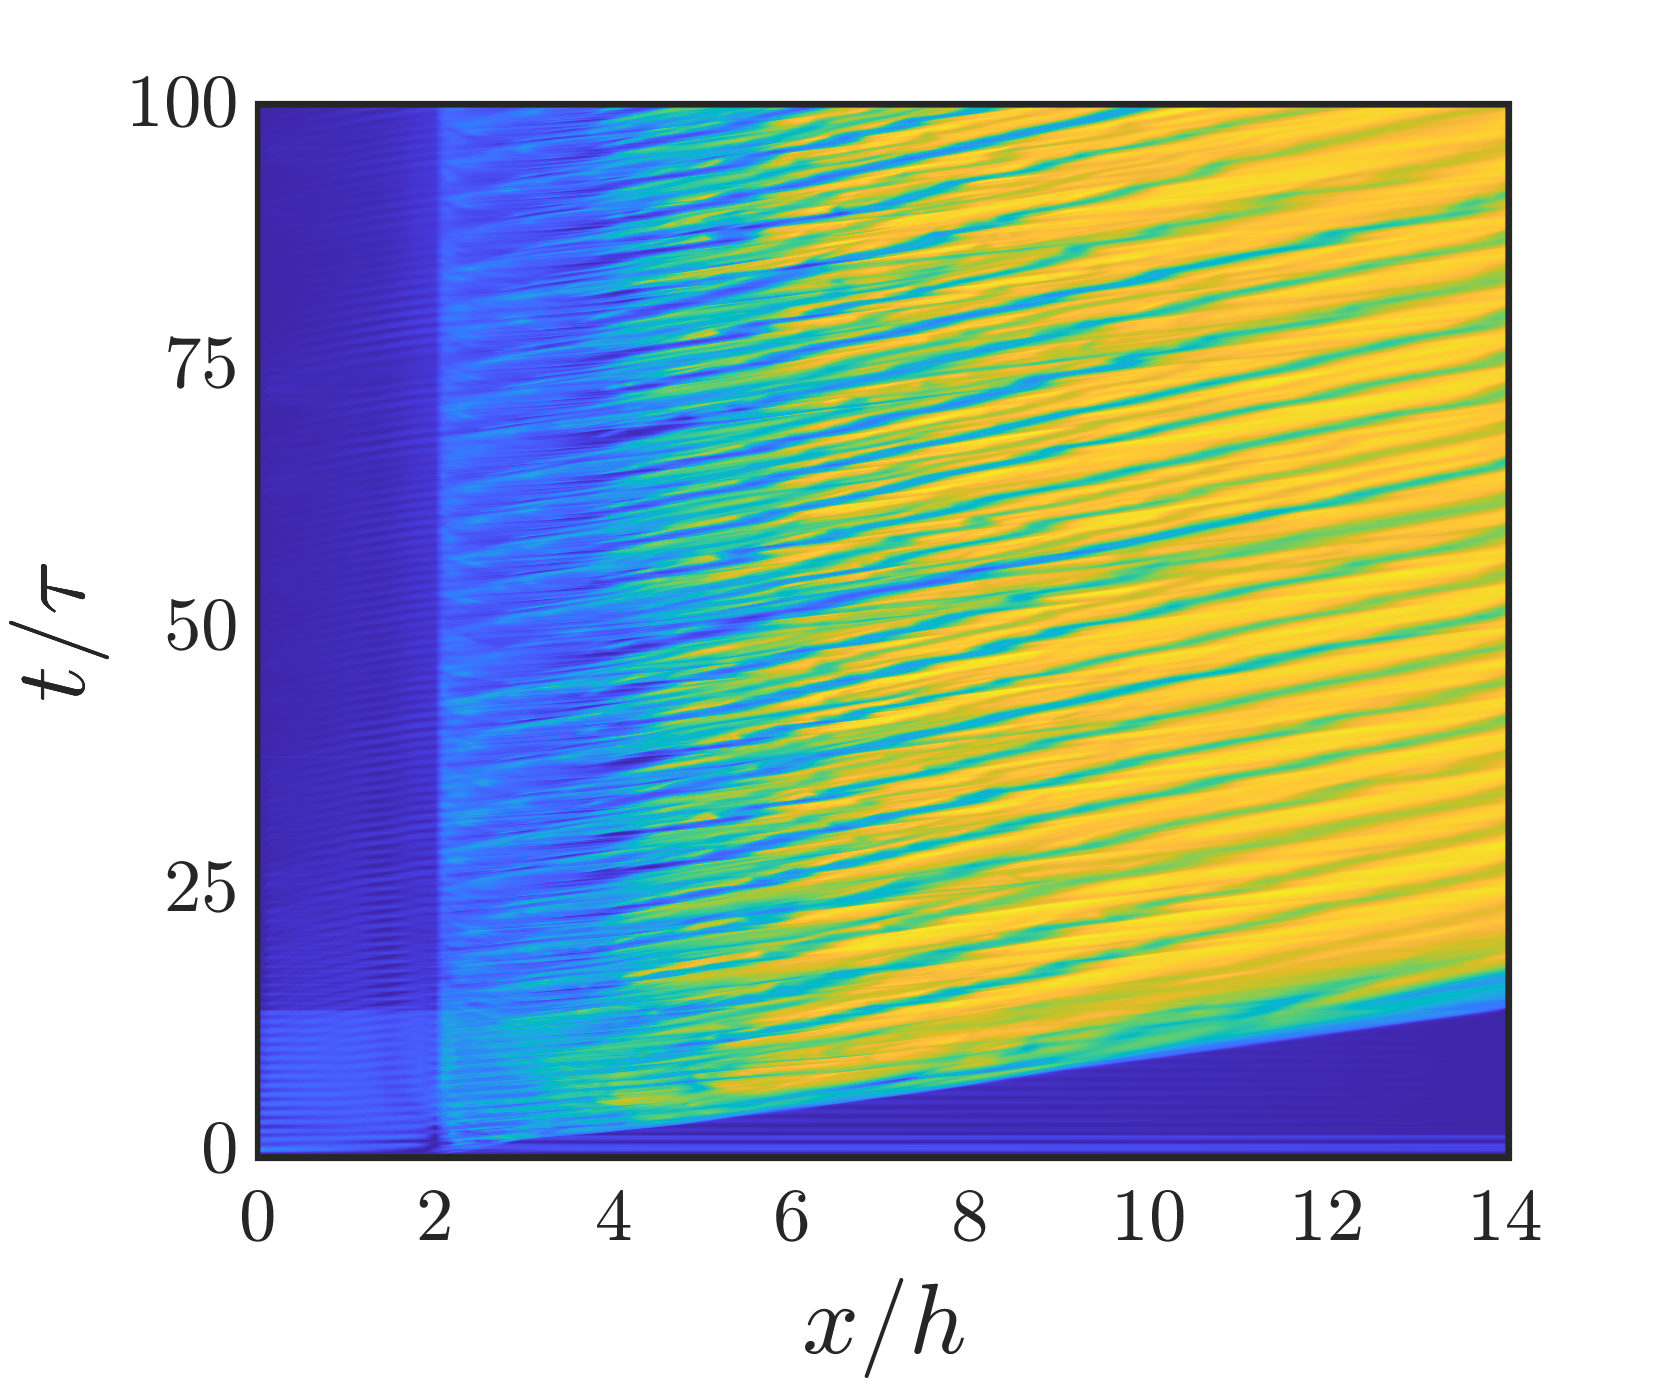
\includegraphics[width=1\linewidth]{Figures/MI_HL/spcaeTime_M_Singled.png}
				%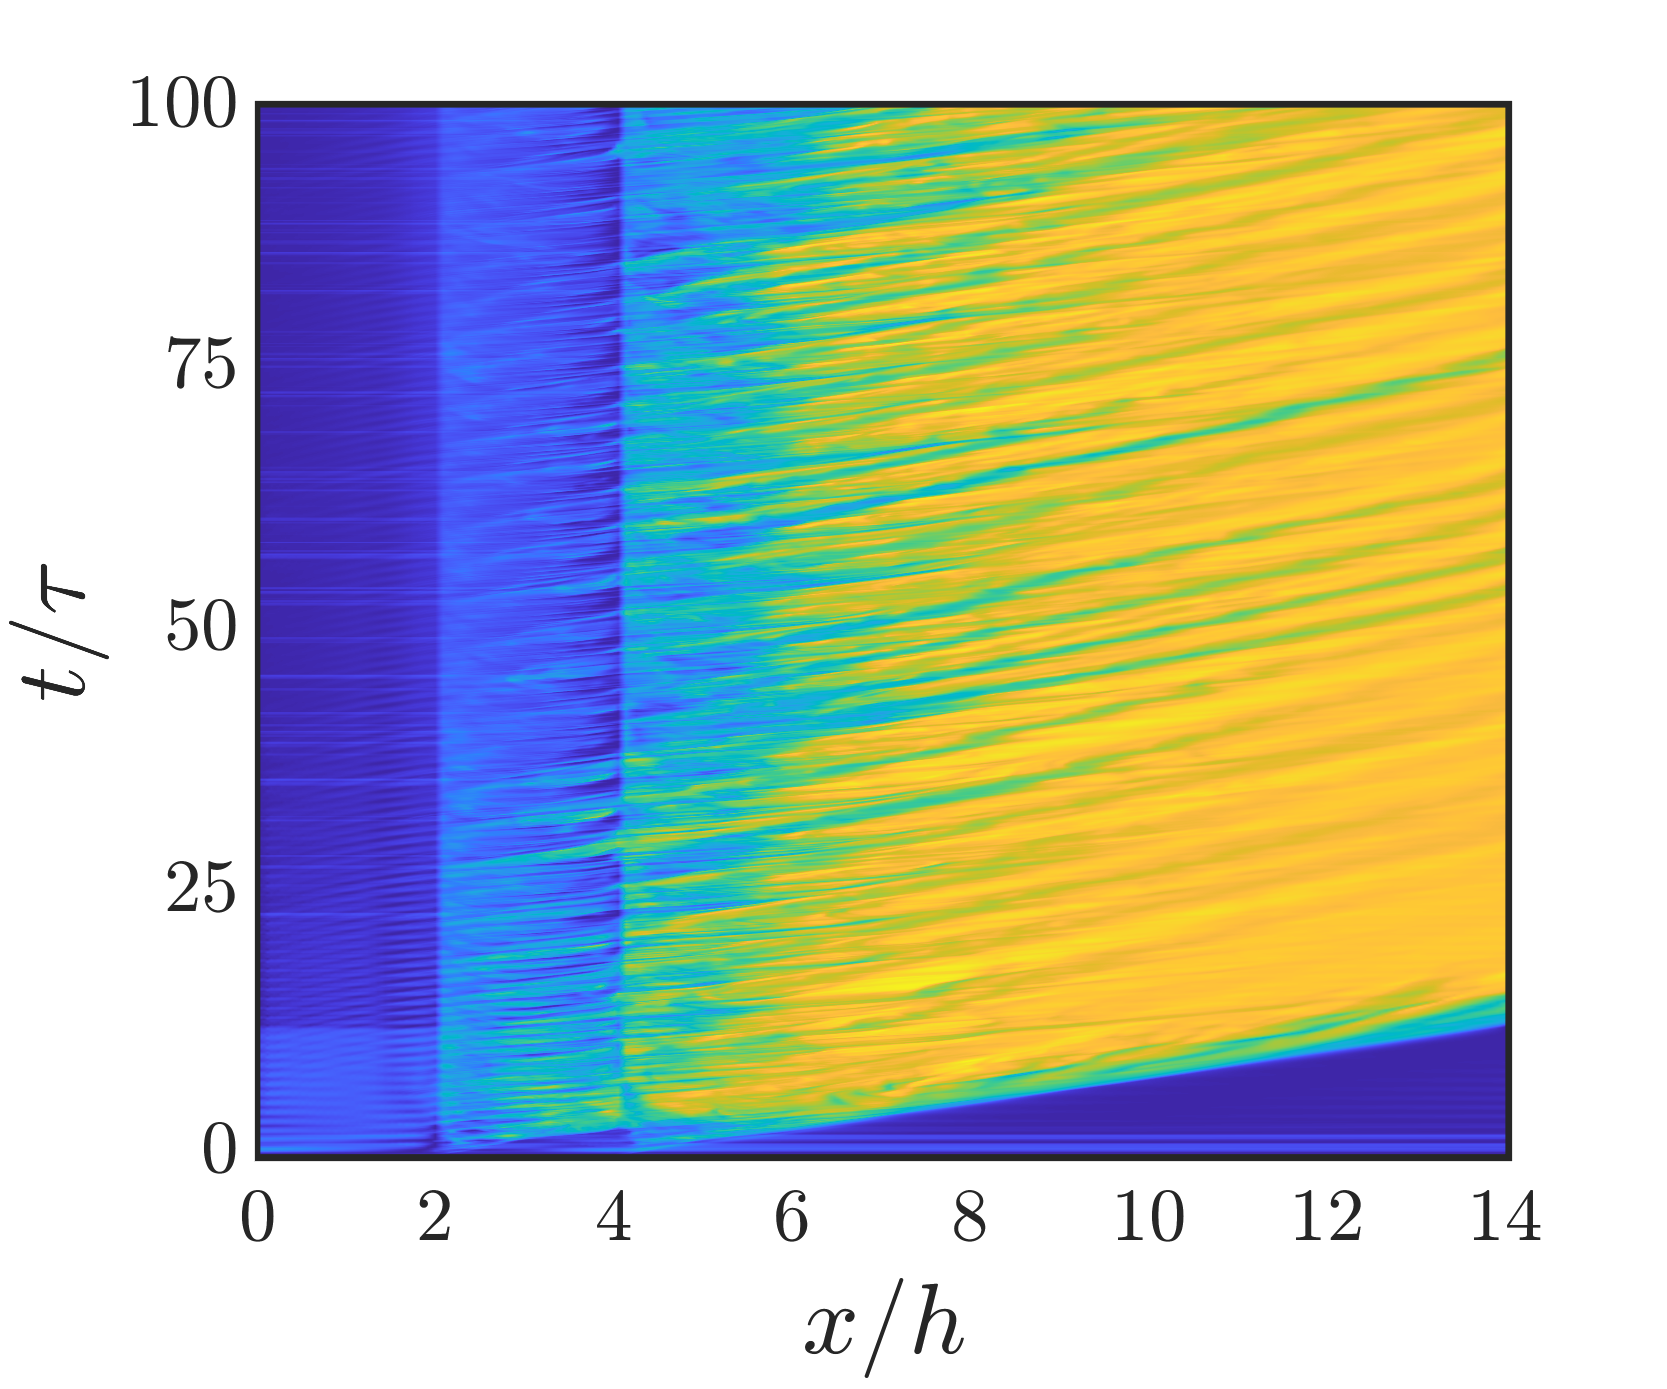
\includegraphics[width=1\linewidth]{Figures/MI_HL/spcaeTime_M_4d.png}
				%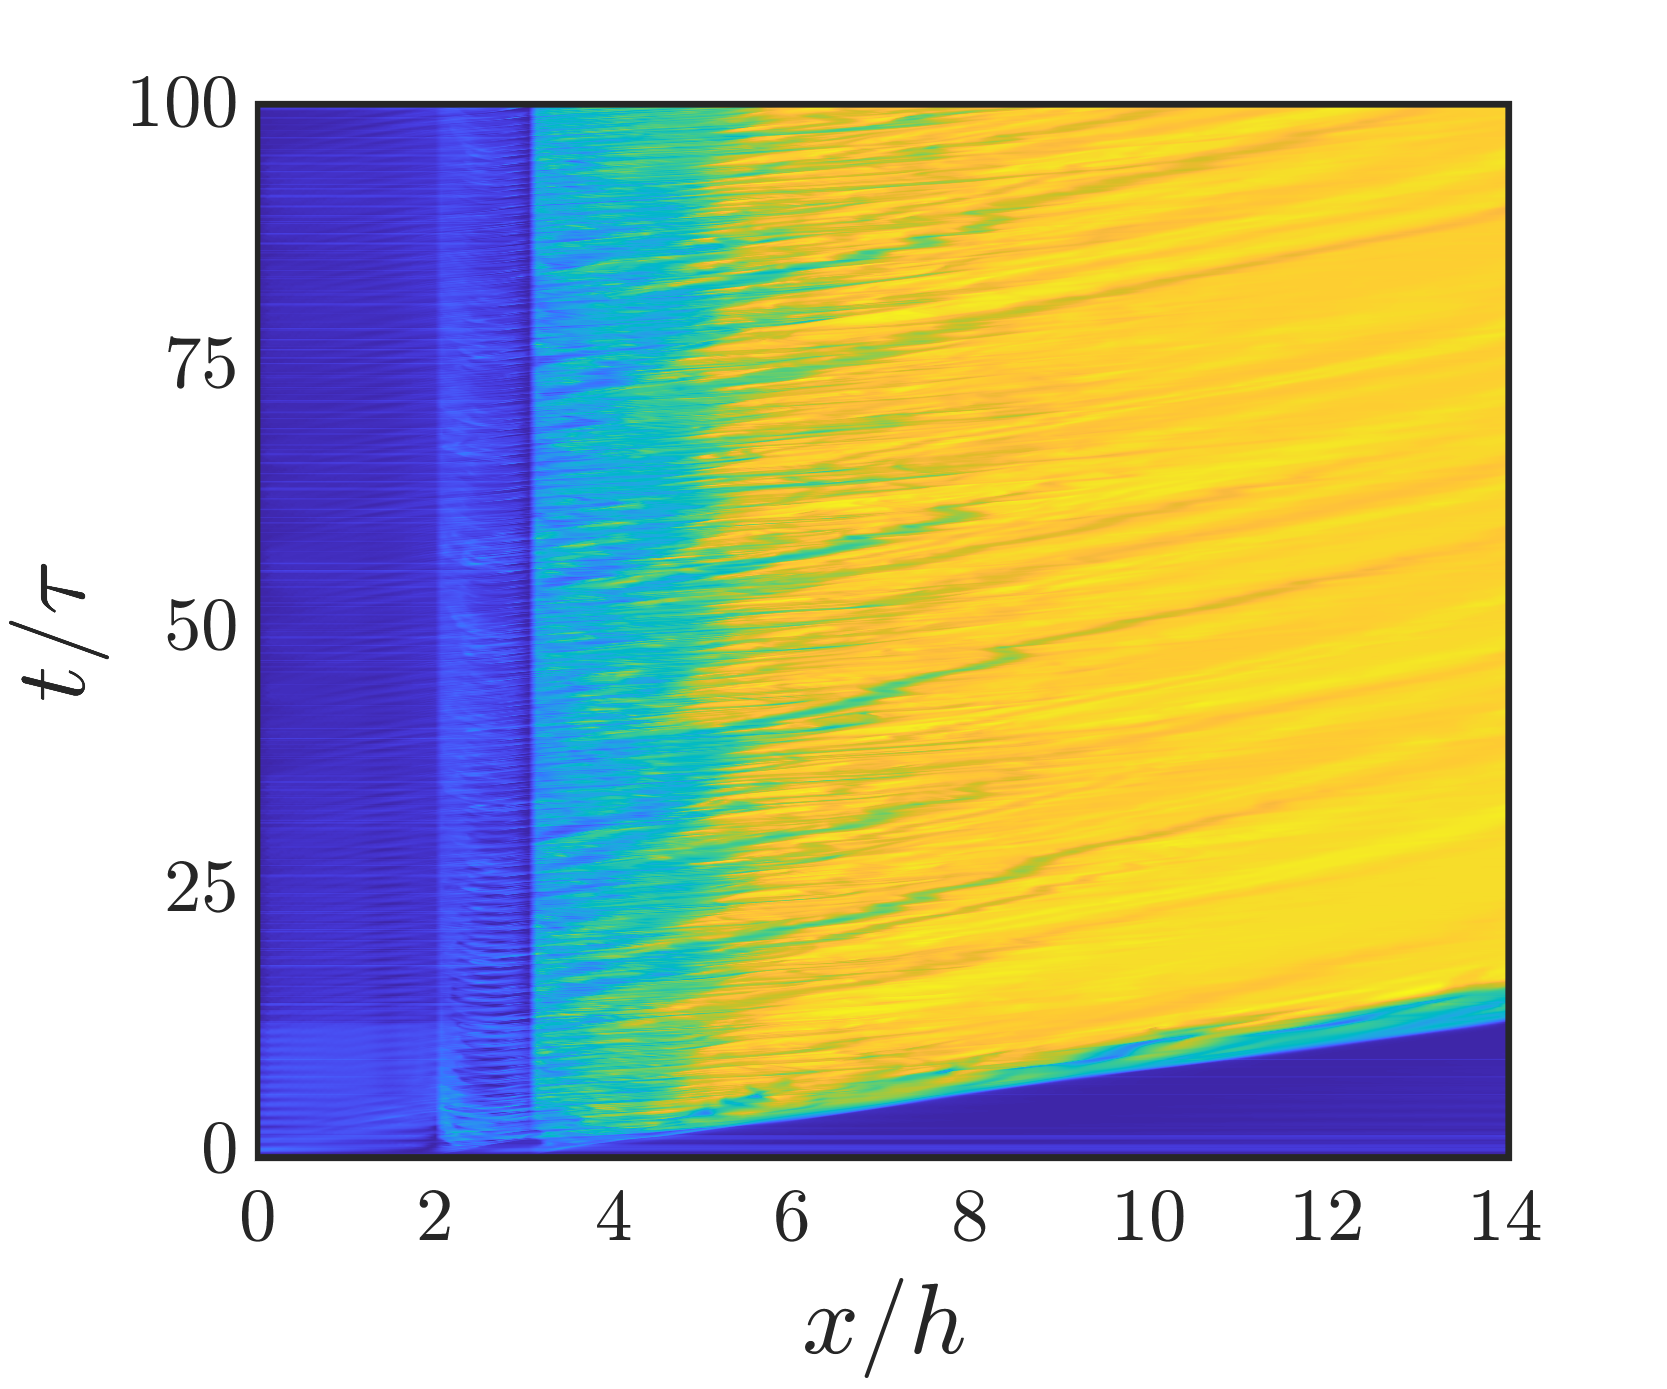
\includegraphics[width=1\linewidth]{Figures/MI_HL/spcaeTime_M_2d.png}
				%%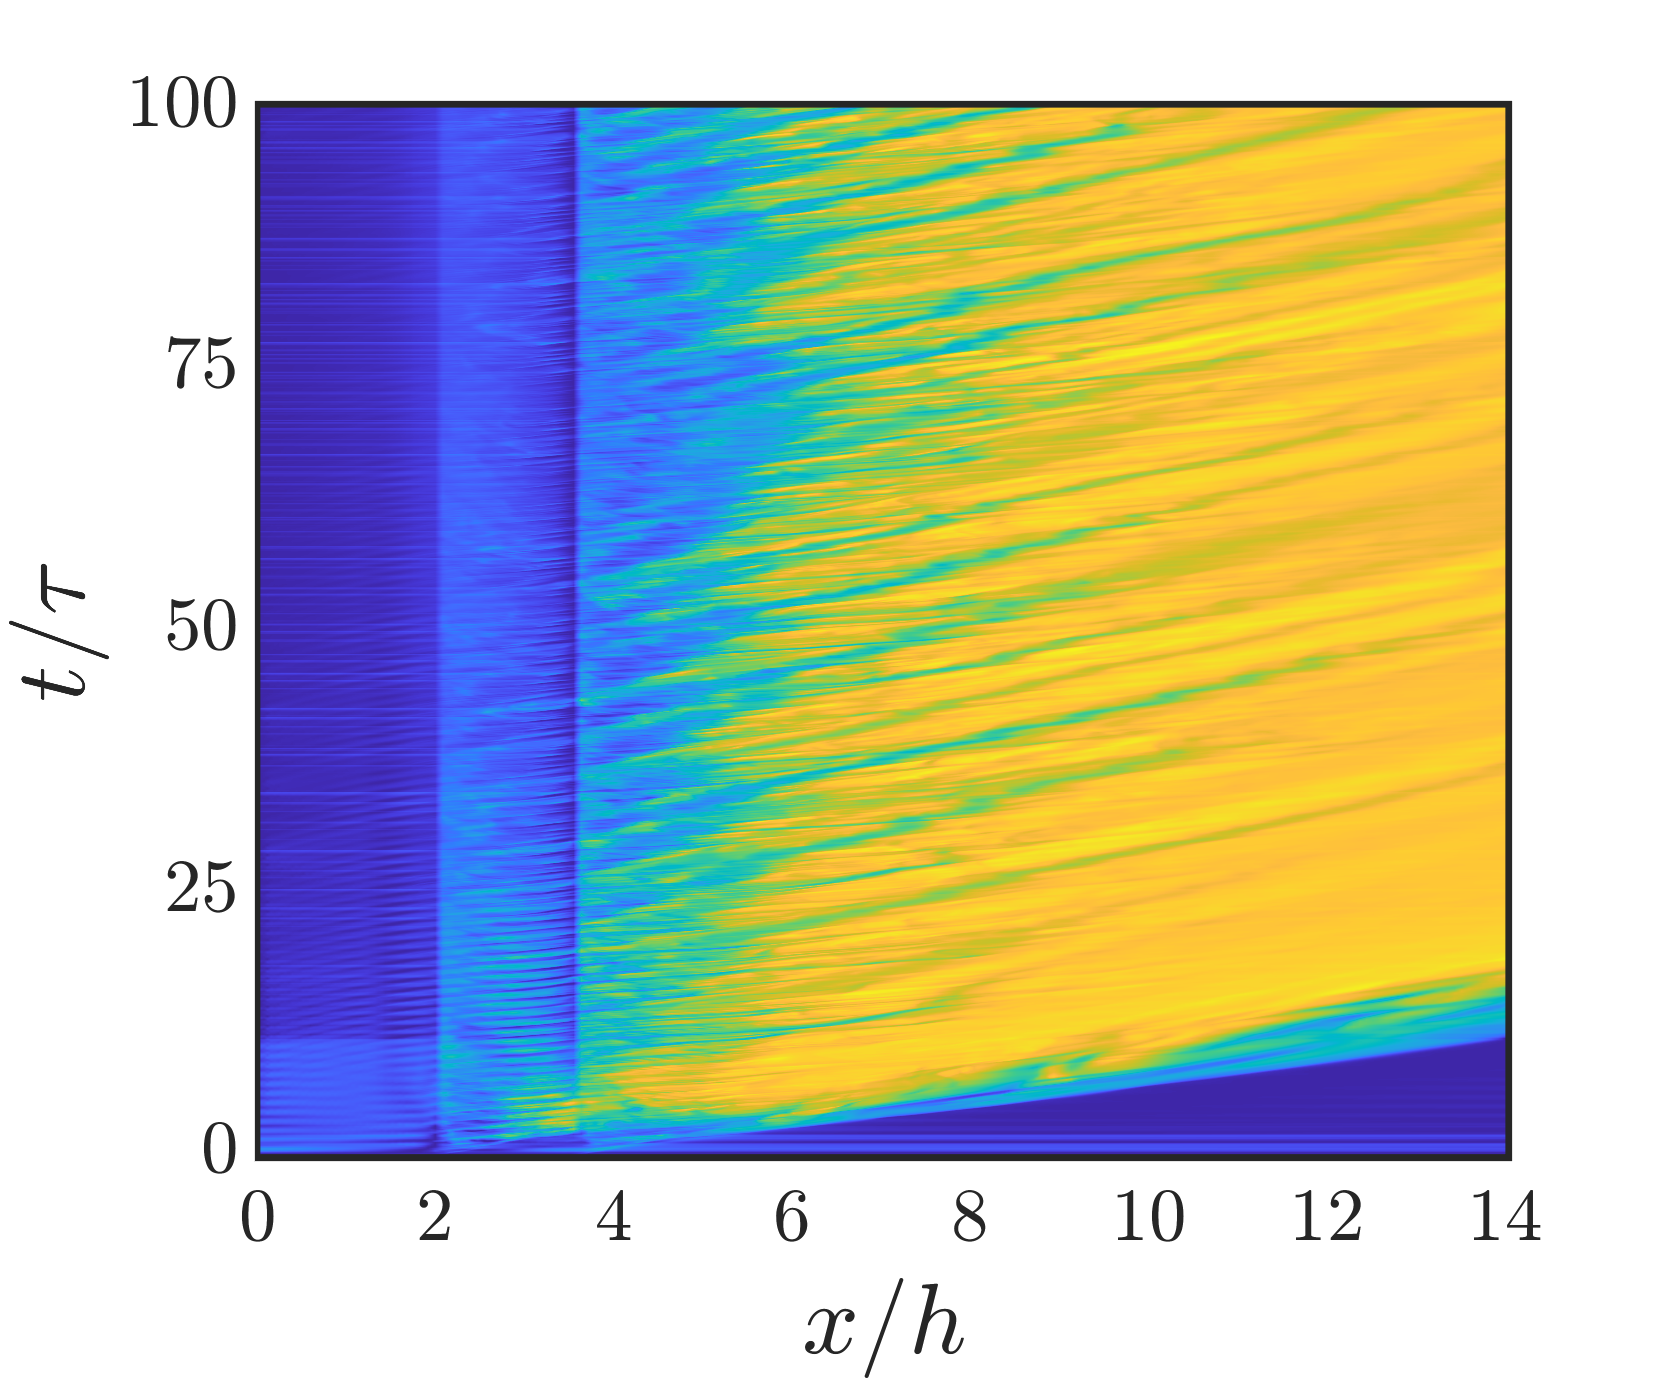
\includegraphics[width=1\linewidth]{Figures/MI_HL/spcaeTime_M_3d.png}
				%%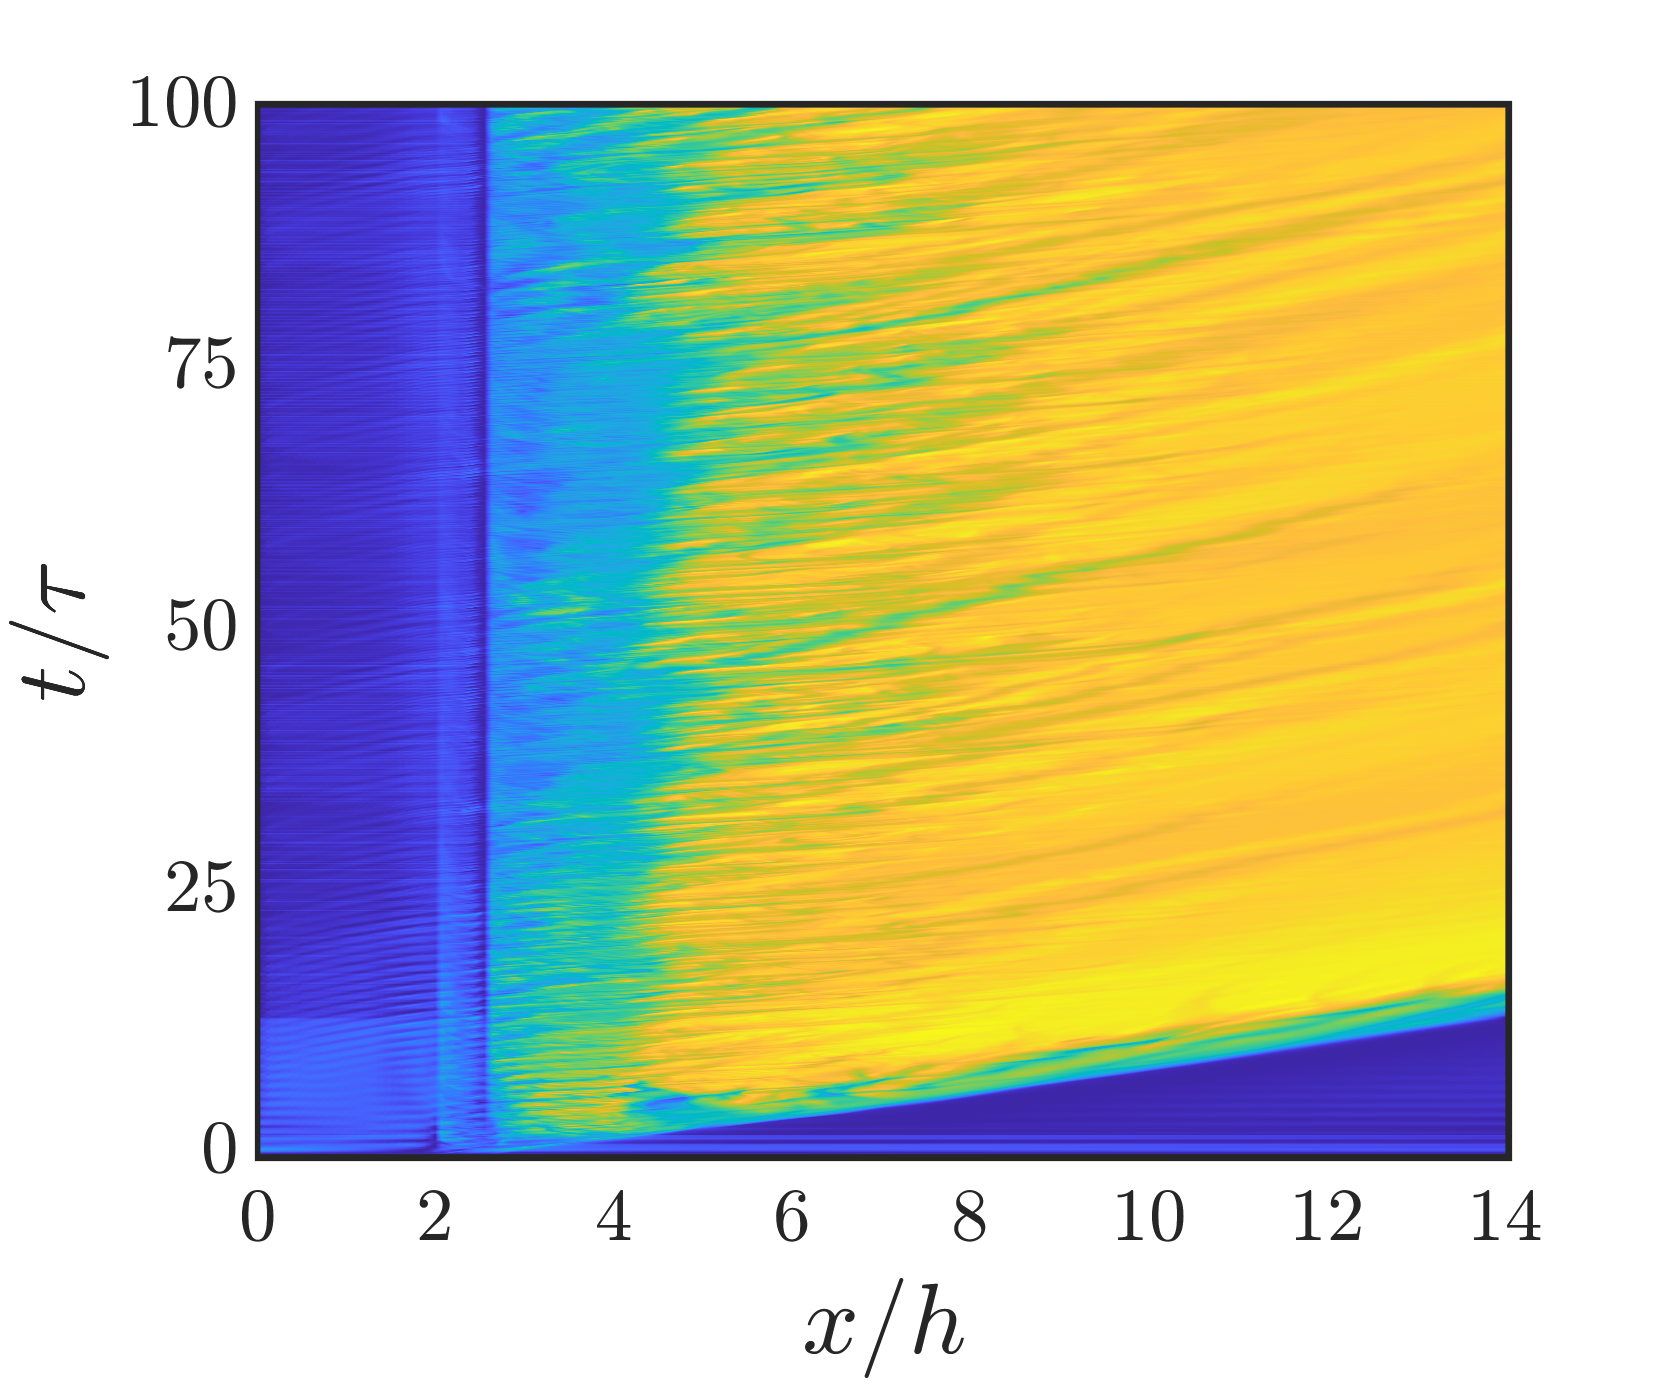
\includegraphics[width=1\linewidth]{Figures/MI_HL/spcaeTime_M_1d.png}
				%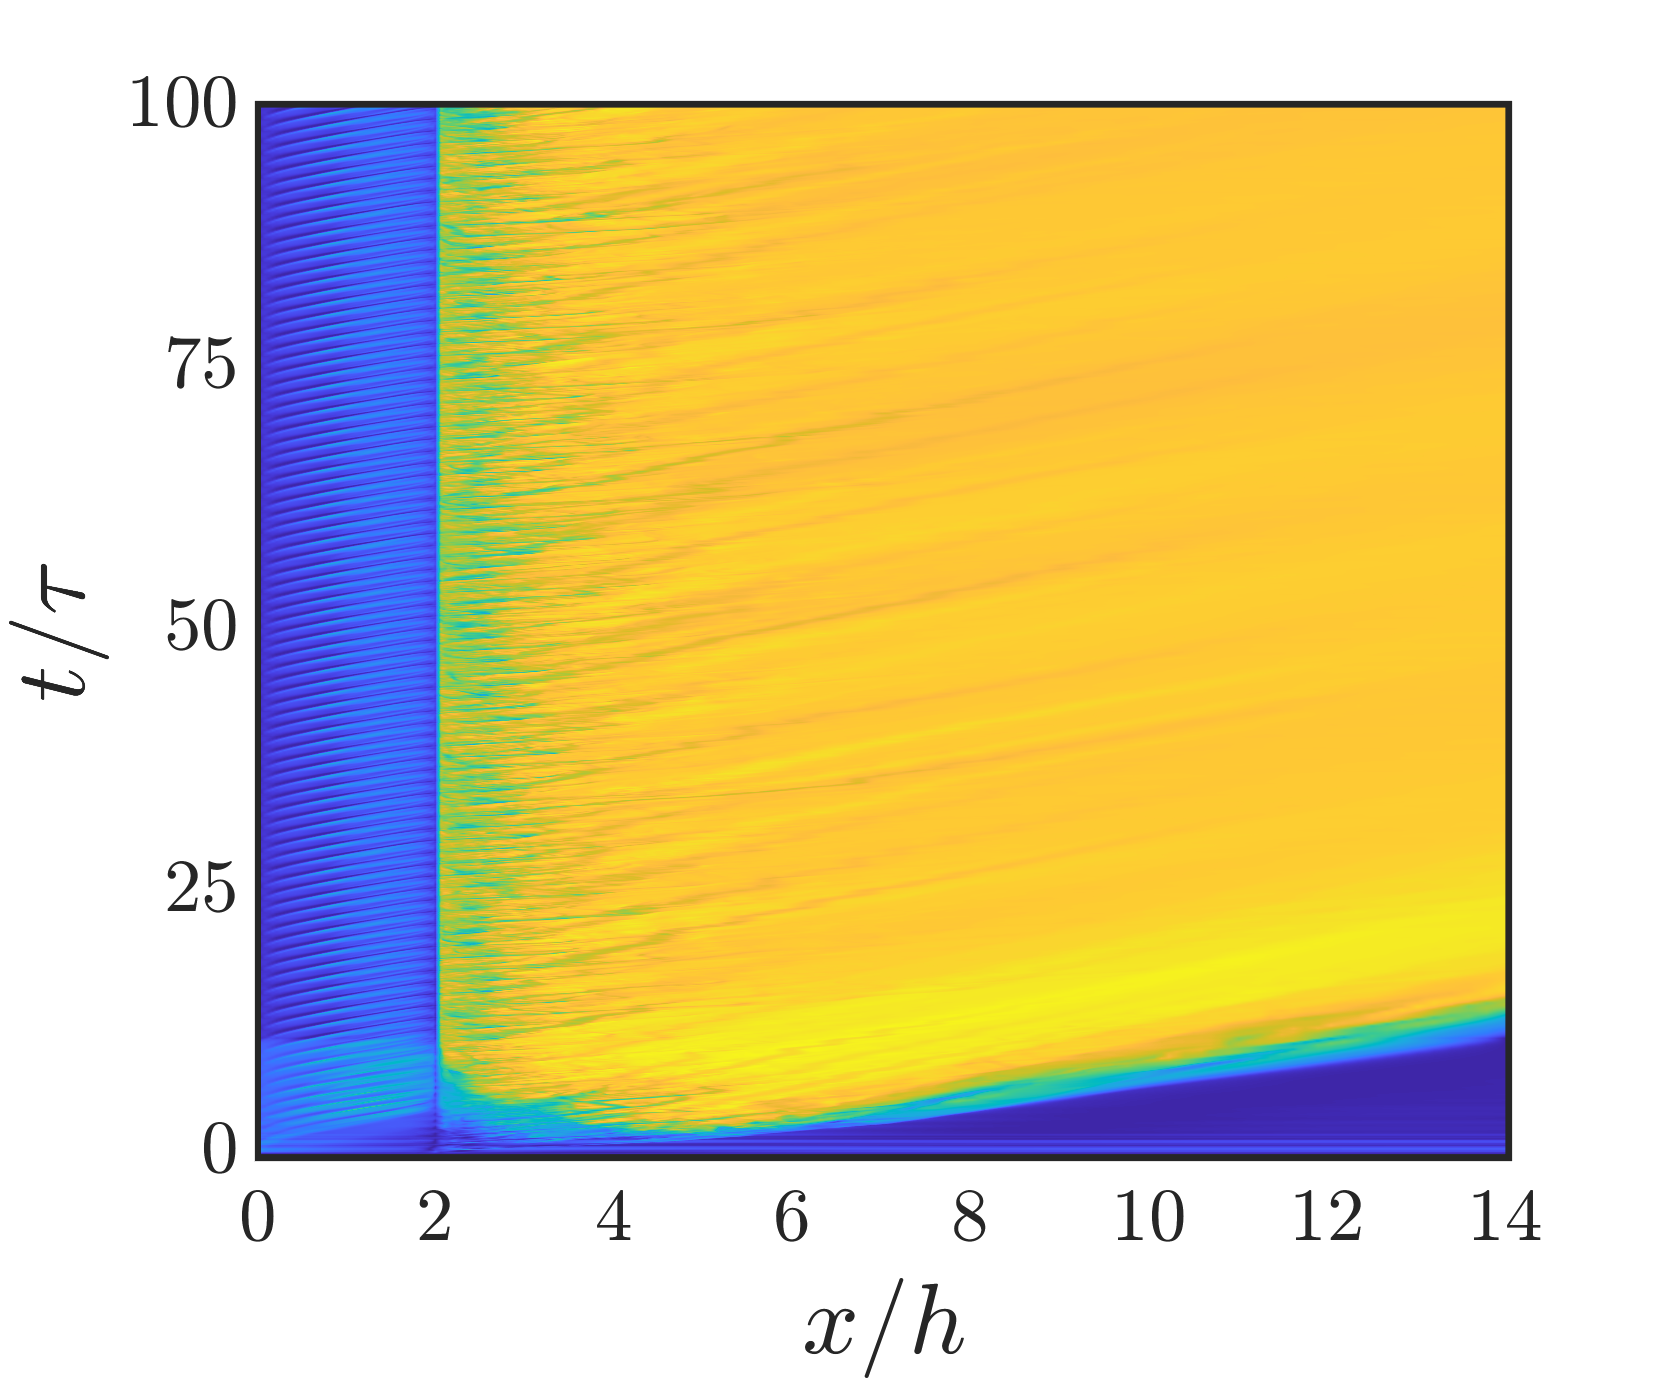
\includegraphics[width=1\linewidth]{Figures/MI_HL/spcaeTime_M_0d.png}
				%	\end{minipage}
			\begin{minipage}[c]{0.24\linewidth}
				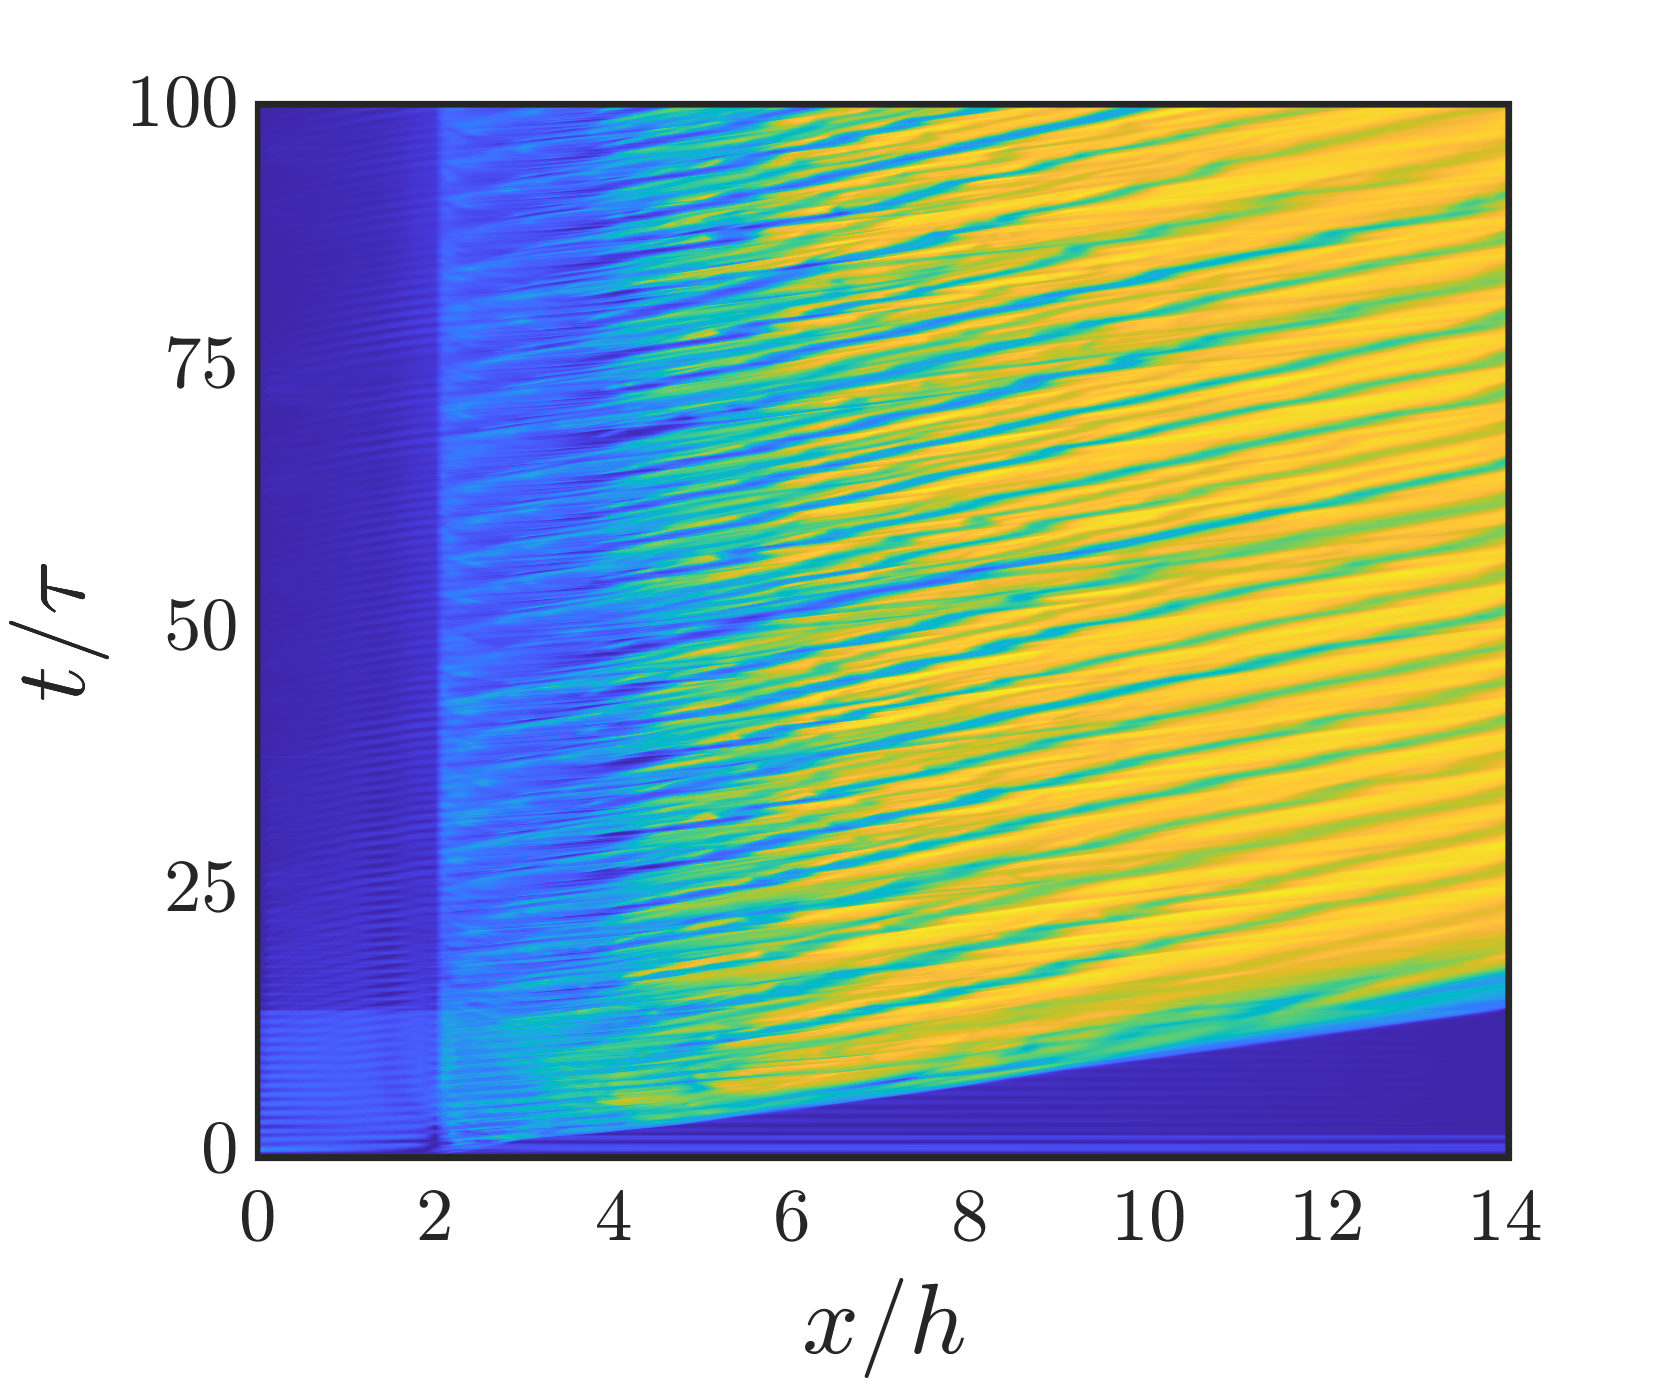
\includegraphics[width=1\linewidth,trim={1.6cm 2cm 2cm 1cm},clip]{Figures/MI_HL/spcaeTime_M_Singled.png}
				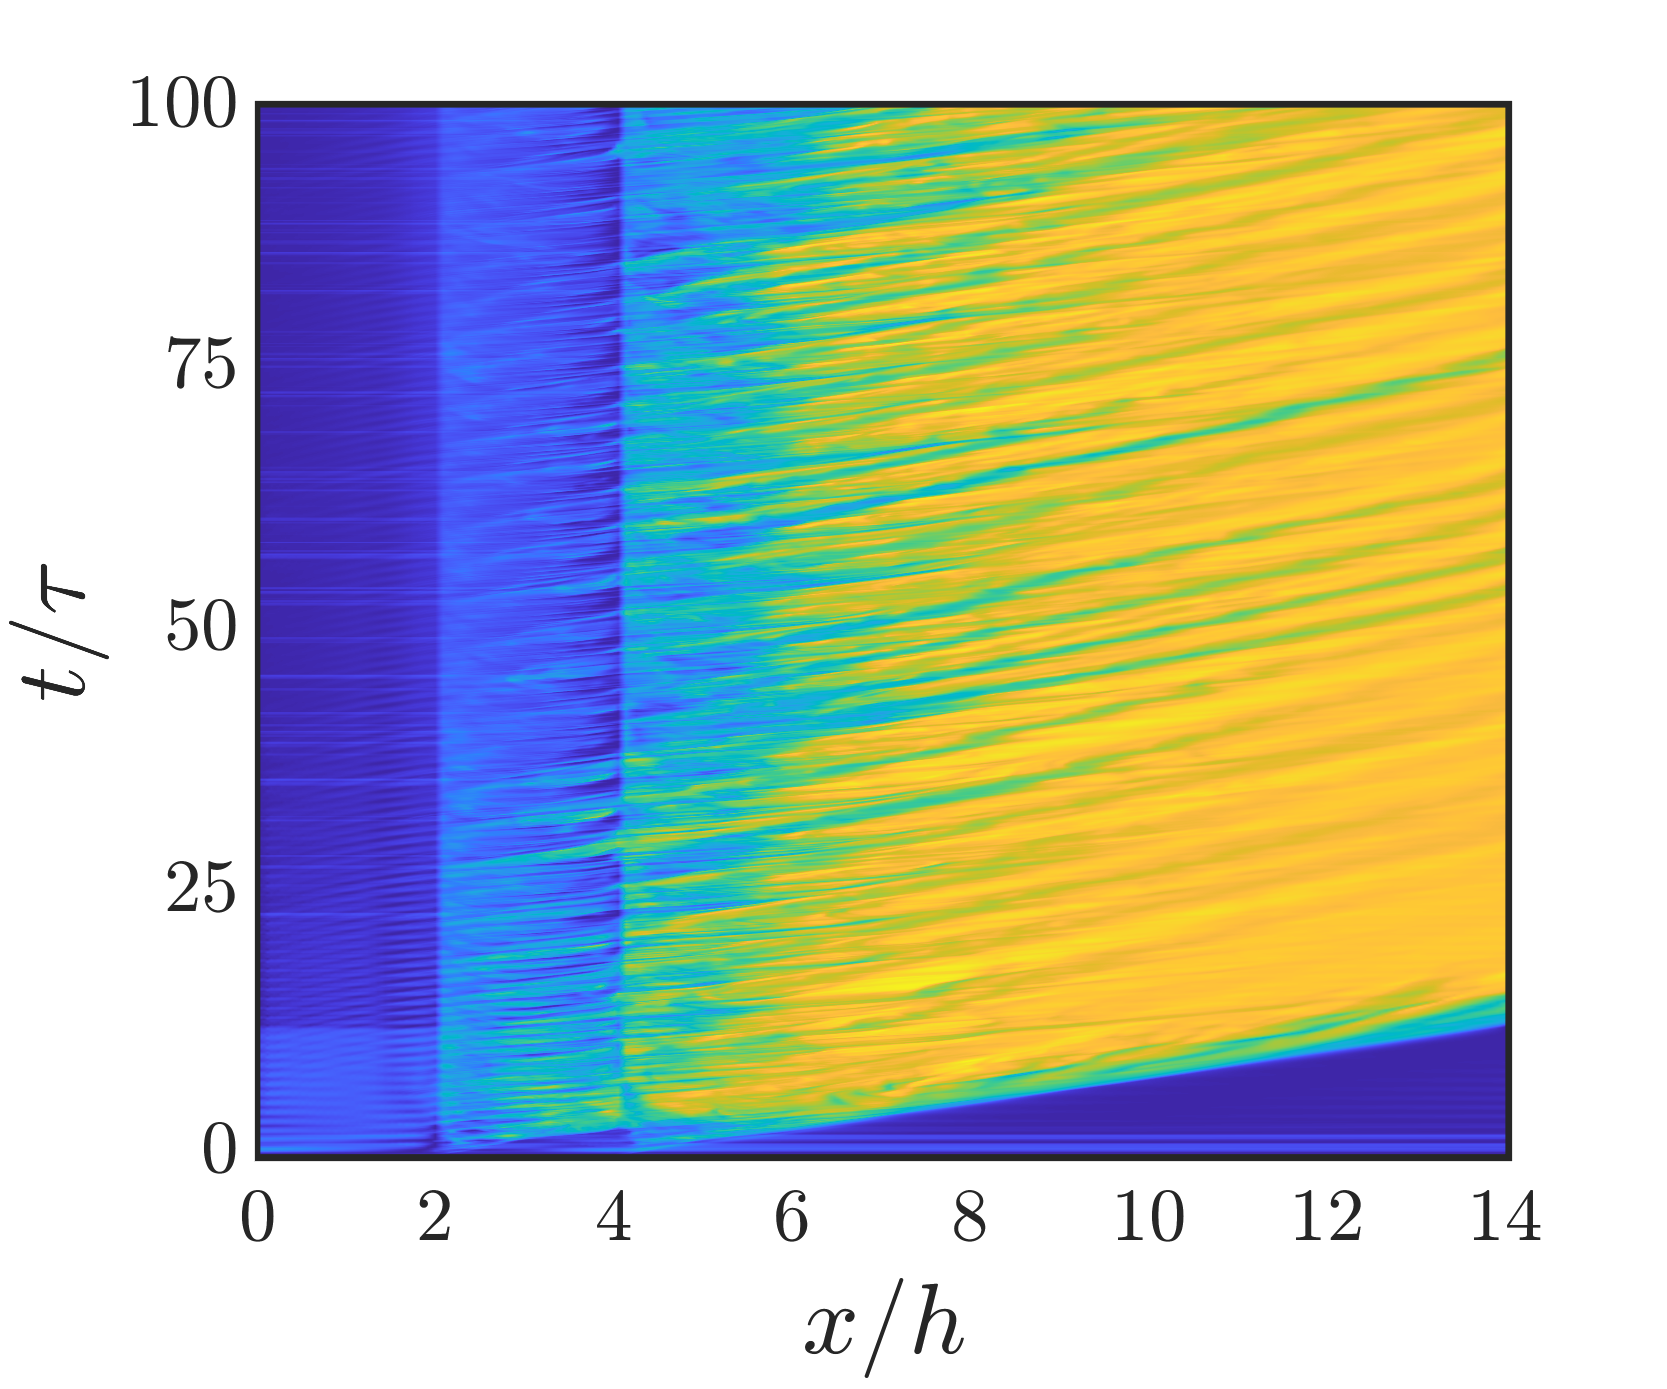
\includegraphics[width=1\linewidth,trim={1.6cm 2cm 2cm 1cm},clip]{Figures/MI_HL/spcaeTime_M_4d.png}
				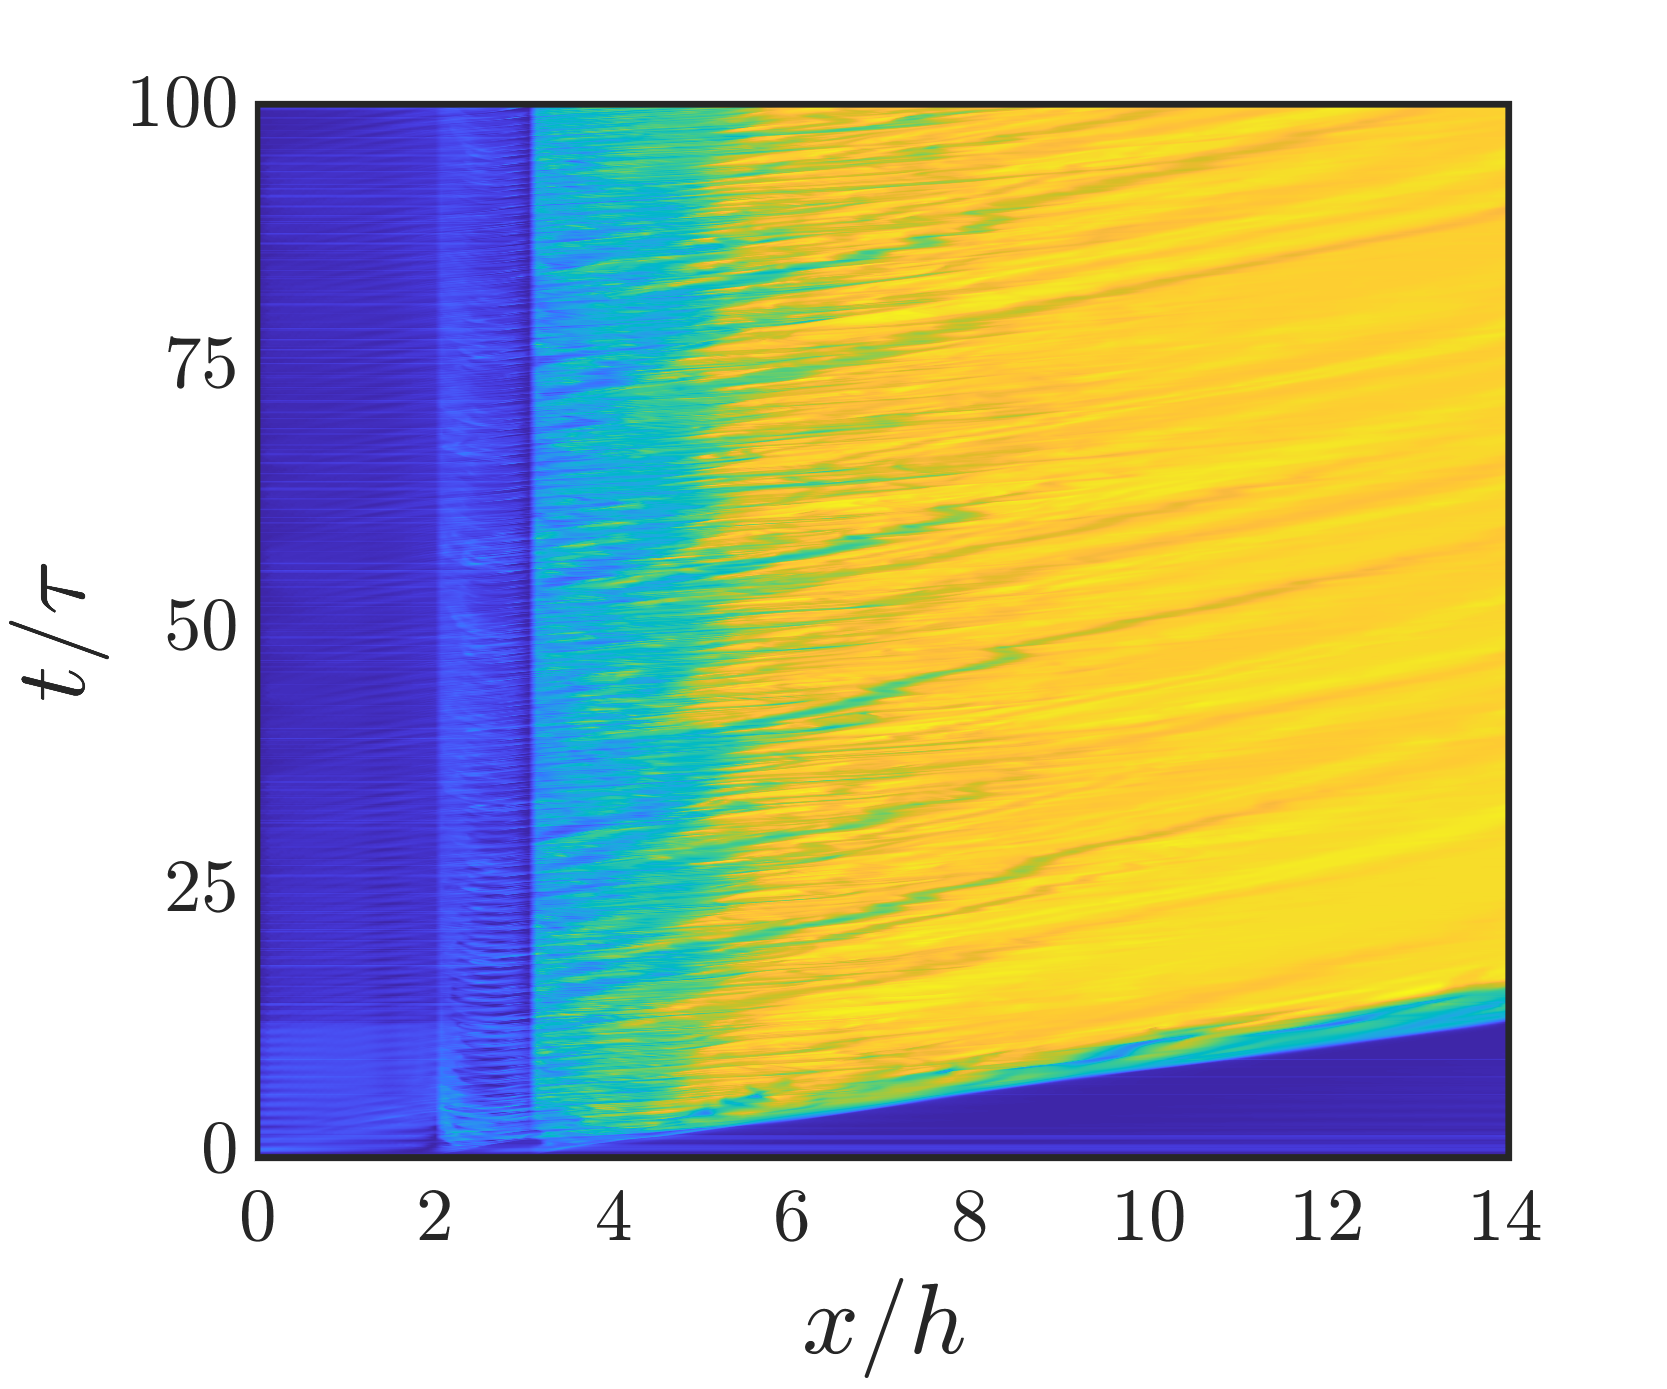
\includegraphics[width=1\linewidth,trim={1.6cm 2cm 2cm 1cm},clip]{Figures/MI_HL/spcaeTime_M_2d.png}
				%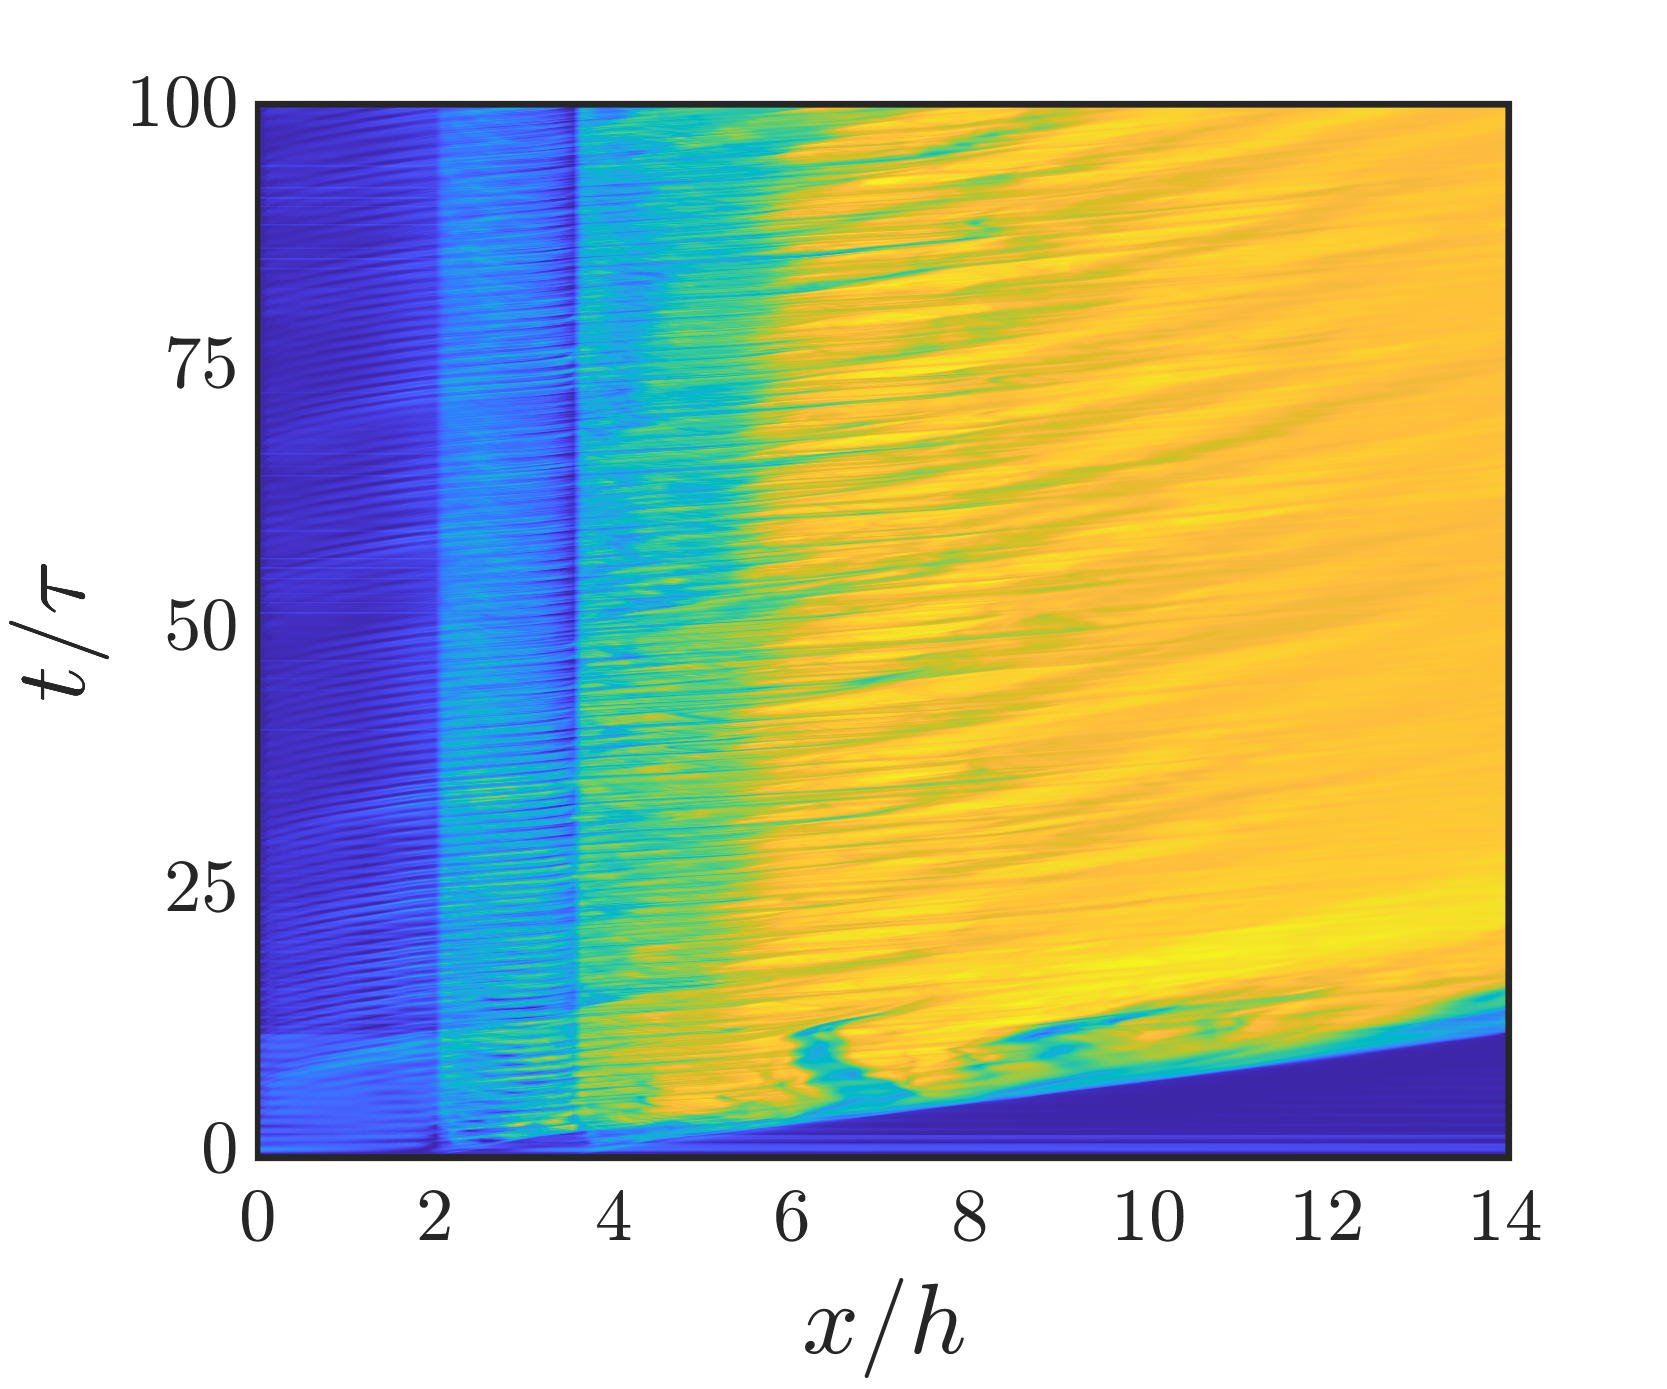
\includegraphics[width=1\linewidth]{Figures/MI_HL/spcaeTime_M_3e.png}
				%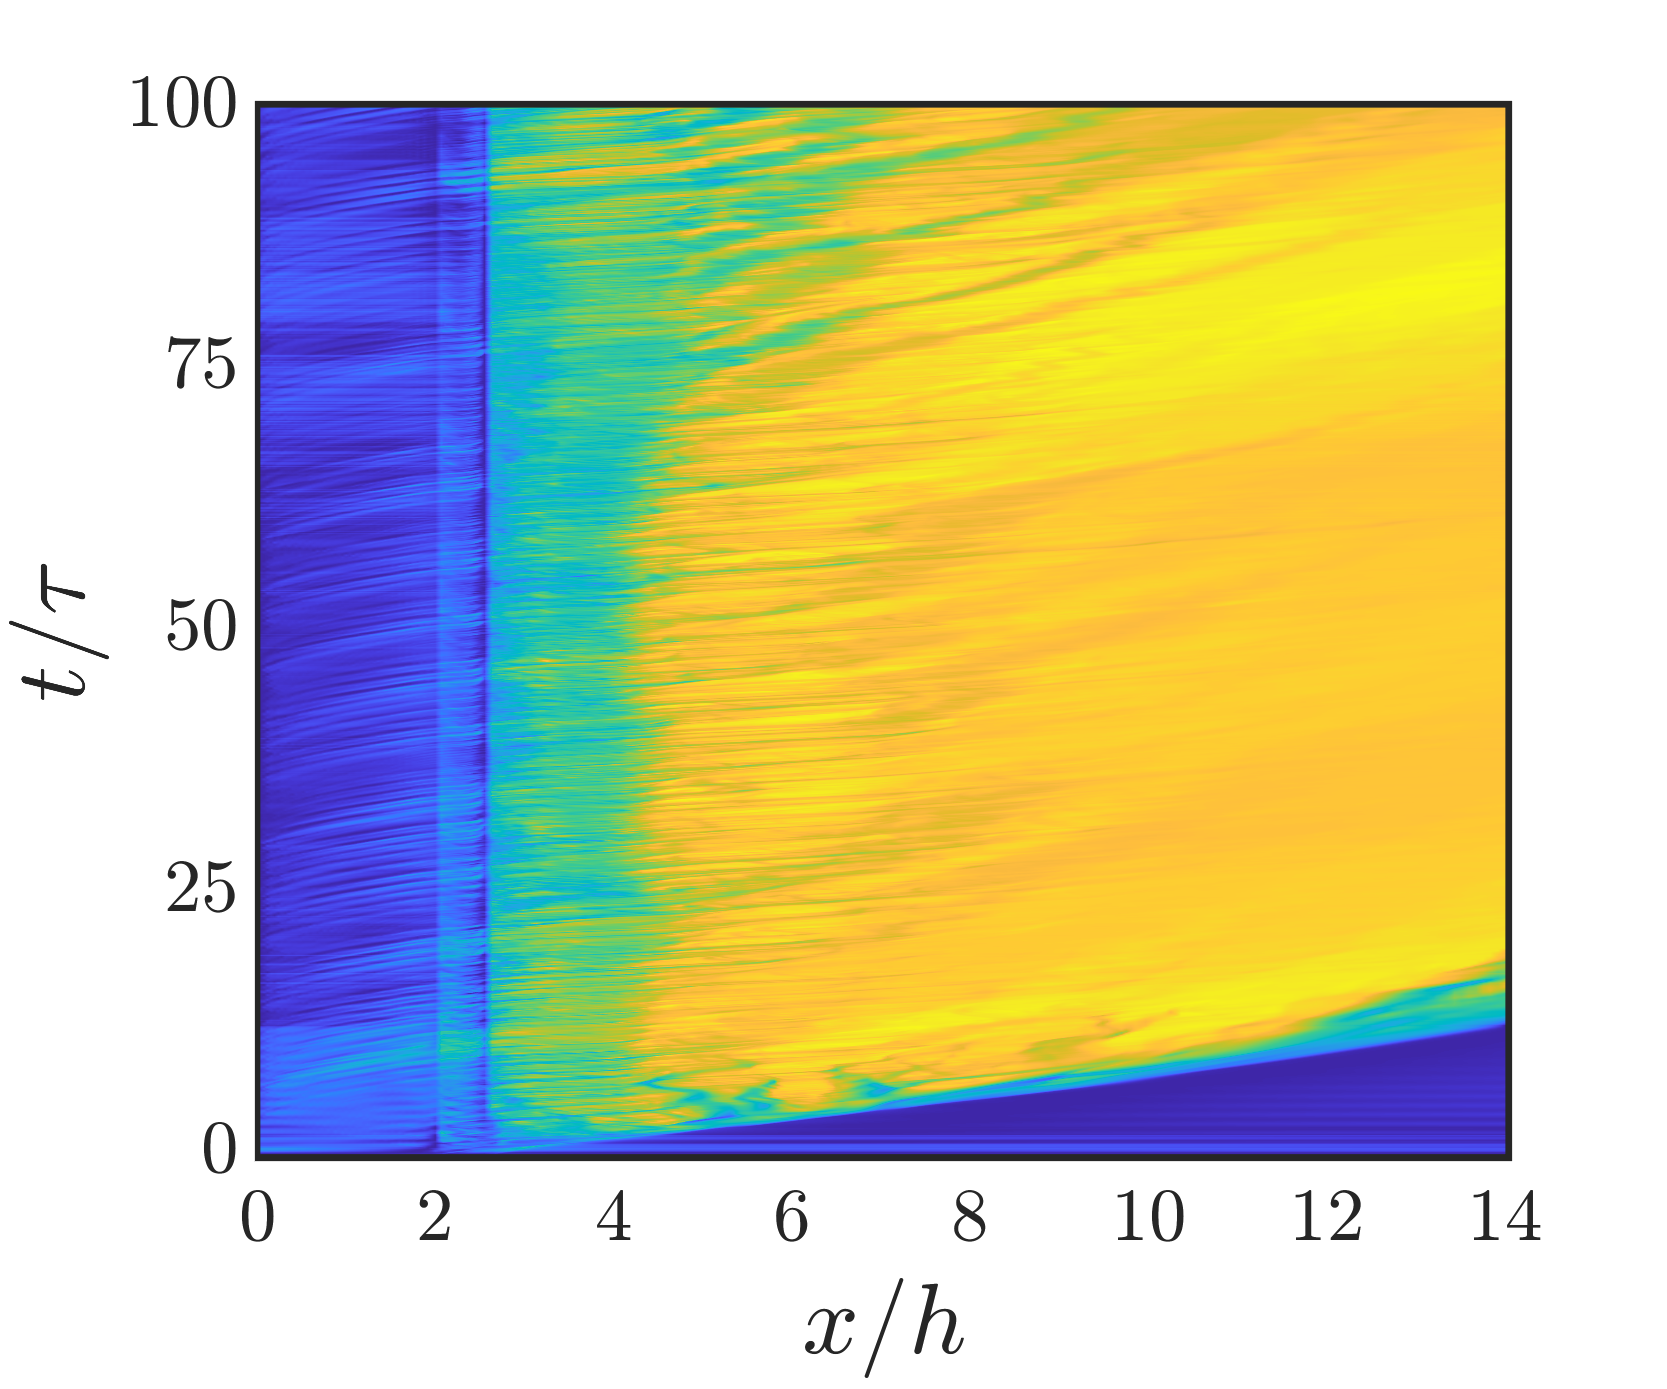
\includegraphics[width=1\linewidth]{Figures/MI_HL/spcaeTime_M_1e.png}
				
				\begin{overpic}[width=1\linewidth,trim={1.6cm 2cm 2cm 1cm},clip]{Figures/MI_HL/spcaeTime_M_0d.png}
					\put(-382,350){{\parbox{1\linewidth}{\rotatebox{90}{\large$single$}}}}	
					\put(-382,250){{\parbox{1\linewidth}{\rotatebox{90}{\large$d/h=2$}}}}
					\put(-382,152){{\parbox{1\linewidth}{\rotatebox{90}{\large$d/h=1$}}}}	
					\put(-382,50){{\parbox{1\linewidth}{\rotatebox{90}{\large$d/h=0$}}}}	
					
					\put(-370,350){{\parbox{1\linewidth}{\rotatebox{90}{\large$t/\tau$}}}}	
					\put(-370,250){{\parbox{1\linewidth}{\rotatebox{90}{\large$t/\tau$}}}}
					\put(-370,152){{\parbox{1\linewidth}{\rotatebox{90}{\large$t/\tau$}}}}	
					\put(-370,55){{\parbox{1\linewidth}{\rotatebox{90}{\large$t/\tau$}}}}
					
					\put(-320,397){{\parbox{1\linewidth}{\large$Re=200$}}}
					\put(-200,397){{\parbox{1\linewidth}{\large$Re=400$}}}
					\put(-80,397){{\parbox{1\linewidth}{\large$Re=800$}}}
					\put(35,397){{\parbox{1\linewidth}{\large$Re=1600$}}}
					
					\put(-10,-10){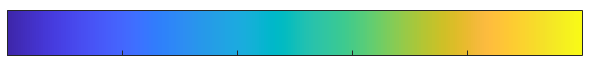
\includegraphics[width=0.85\linewidth]{Figures/MI_HL/leg_timespace.png}}
					%			\put(110,-20){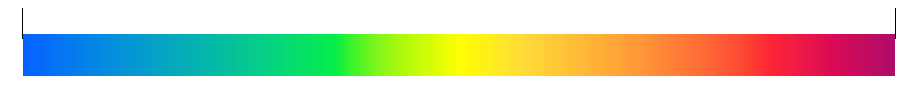
\includegraphics[width=0.45\linewidth]{Figures/legend_scalar.png}}
					\put(32,-10){{\parbox{1\linewidth}{$MI$}}}	
					\put(96,-10){{\parbox{1\linewidth}{$1$}}}
					\put(-20,-10){{\parbox{1\linewidth}{$0$}}}	
					
					\put(-310,-6.5){{\parbox{1\linewidth}{$x/h$}}}
					\put(-185,-6.5){{\parbox{1\linewidth}{$x/h$}}}
					\put(-65,-6.5){{\parbox{1\linewidth}{$x/h$}}}
					\put(55,-6.5){{\parbox{1\linewidth}{$x/h$}}}			
				\end{overpic}
			\end{minipage}
			\vspace{0.75cm}
			\caption{Timespace map for mixing index $(MI)$ for single and $d/h=0,1,2$ cases (row-wise), and for $Re=200,400,800,1600$ cases (column-wise). See animation \citep{animation} for better understanding.}
			\label{fig:spaceTime}
		\end{figure*}
		
		The plates' deflection under the fluid load generates complex flow features due to the mutual interplay of forces. In Figure \ref{fig:contour_single}(a), we have shown instantaneous iso-contours of flow vorticity for single plate case at $Re=200-3200$. The flow gets obstructed by the plate and accelerates through the remaining gap, generating vorticity at the top wall and in the form of the plate's tip-attached shear layer. We can notice the roll-up and breakdown of the shear layer upon increasing the $Re$ beyond $200$. The clockwise and counter-clockwise vortex structures generated off the plates' tip and the top wall, respectively, arrange themselves in alternating fashion downstream, which indicates periodic shedding of the vortices off the plate. These vortex structures, as they roll, advect downstream due to the incoming inertia and cause a stirring effect in the fluid, thereby causing the mixing of the two fluids.
		
		
		In Figure \ref{fig:contour_single}(b), we have shown two scalar concentration fields $\phi=0 \& 1$ initially separated distinctly into top-half and bottom-half, distinctly. For $Re=200$, the instantaneous scalar field remains largely unmixed due to the flow disturbances as the single plate achieves static reconfiguration mode with negligible flutter amplitude, which does not impact the shear layer breakup. However, for $Re\geq 400$, we can observe a transition in the mixing of the scalar as the aforementioned vortices agitate the field more and more with increasing $Re$. These vortices entrain the scalar into their field and for localized mixing zones, increasing the mixing by diffusion. In the case with $Re=3200$, we can note that the flow near the inlet also transitions towards a turbulent field even before interacting with the plates. 
		
		The mixing of the scalar field can be statistically evaluated by many methods used in the past \citep{Danckwerts1952, Liscinsky1993, Kockmann2006}. We have used the infamous statistical method for estimating mixing known as the `Mixing Index', which in our work can be expressed along the channel downstream length as
		\begin{equation}
			MI(x)=1-\sqrt{\frac{\sigma(x)^2}{{\sigma^2_{max}}}},
		\end{equation}

		\begin{equation}
		where, \sigma(x)=\sqrt{{1\over h} \int_{0}^{h} [\phi(x,y)-\phi_m]^2 \,dy}
		\end{equation}
		
		where $\sigma(x)$ is the standard deviation of the vertically integrated scalar field across the channel, $\phi_m$ is the mean of the scalar concentration field or scalar concentration value for a fully mixed solution, and $\sigma_{max}$ is the maximum deviation in the scalar concentration field. According to this method, the `Mixing Index' ranges from $0$ to $1$ where $MI=1$ represents a completely mixed solution and $MI=0$ represents the fully unmixed scalar field. We have accounted for a value-for-cost analogy in our work, where $MI$ is considered the final value, which shall come at a cost. We have considered the head loss in the channel flow caused by the presence of flexible obstructions as the cost for the value. We have computed head loss along the channel by vertically (across the channel length) integrating the mechanical head along the channel and subtracting from the initial pressure, which is expressed as:
		\begin{equation}
			\mathcal{H}(x)=\frac{1}{h}\int_{0}^{h}[p(x,y)+{1\over2}  u_f^2(x,y)]dy;  
		\end{equation}
		
		\begin{equation}
			\mathcal{H}^*(x)=\frac{\mathcal{H}(x)}{\rho_f \overline{U}^2}; \text{Head Loss}, HL(x) = \mathcal{H}^*(0)-\mathcal{H}^*(x)
		\end{equation}
		
		In Figure \ref{fig:MI_Single}(a), we show $MI(x)$ for the single plate case for different $Re$. The grey rectangle in the figure marks the streamwise position of the plate in the channel for reference. As suggested in the contour plots, we see that mixing for $Re=200$ case is much lower than the higher $Re$ cases. For $Re\geq400$, the $MI$ shoots high in the channel downstream as early as $x=5h$. We have also simulated an empty channel flow, i.e., no obstruction, with the same scalar field configuration for the $Re$ range for reference. The dashed curves in the plot show $MI$ for the empty channel case following the same color codes for the $Re$ case. We can notice that the $MI(x)$ in an empty channel follows a linear trend for $Re\leq1600$, whereas in the case with $Re=3200$, the flow destabilizes into the transition zone, and a non-linear $MI(x)$ curve can be observed.
		
		In Figure \ref{fig:MI_Single}(b), we have shown the total mechanical head loss, $HL$, for a single plate case along the channel streamwise direction for varying $Re$. The $HL$ spikes up near the plate due to the sudden obstruction of the flow inertia and then decays to a nearly constant value as the flow improves downstream. Despite the difference in $MI$ for varying $Re$, $HL$ value does not vary significantly with $Re$ near the exit. We have also shown $HL$ for the empty channel case for reference, and an increasing slope in the linear trend can be observed for decreasing $Re$.
		
		
		With an initial analysis of the single plate case, we extend our study further by introducing the second plate downstream. In figure \ref{fig:contour_800}(a), instantaneous vorticity iso-contours are shown for single and two plate configurations with $d/h=2,1.5,1,0.5,0$ at $Re=400$. The presence of another plate contributes to more vorticity than the single plate case as plate 2 assists the top wall shear layer to shed periodically of its tip. When plate 2 is placed even closer, the vortex shedding off both plates' tips is more frequent and intense because of its effective flow blockage. In figure  \ref{fig:contour_800}(b), the instantaneous contour for the scalar field is shown for the same set of configurations at $Re=800$. In a single plate case, the flow jumps over the plate, destabilizes, and, in turn, agitates further downstream. With the placement of the second plate on the opposite wall, this flow jump gets constricted as per the location of plate 2, and thus, we can notice the early blending of the two fluids as $d/h$ is decreased. Note that, in $d/h=0$ configuration, the two plates heavily obstruct the flow, disturb the flow even upstream to the plates, and induce slight fluid mixing before the obstruction.
		
		In Figure \ref{fig:MI_400}(a), $MI$ along channel length for the various $d/h$ configurations is compared for $Re=400$ in steady state. As evident by the contour plots before, the $MI$ in the channel shoots up steeply past the plates' location. The grey rectangle marks the location of plate 1 in the channel for reference. We observe that $MI$ at further downstream locations subsequently decreases with increasing $d/h$ with maximum value at $d/h=0$, showing significant mixing ahead of the plates and peak mixing immediately next to the plates. However, this steep mixing curve for $d/h=0$ configuration comes at a high head loss, as shown in figure \ref{fig:MI_400}(b), which features a significant difference from the other configurations. The plot shows expected head loss results as per the flow obstruction configuration, i.e., decreasing $HL$ with increasing plates' separation ($d/h$).
		
		For a comprehensive overview of the development of $MI$ for different configurations under various $Re$, we have shown the time-space plots in figure \ref{fig:spaceTime}. This reveals that at lower $Re$, the $MI$ increases gradually over time, whereas at higher $Re$, we can see early mixing of fluids also increased mixing as the $d/h$ decreases. However, the $d/h=0$ configuration stands out with the highest mixing very early in the channel as well as early in time. Interestingly, the $Re=800$ case exhibits much better mixing results than the $Re=3200$ case for $d/h=0$.
		
		In Figure \ref{fig:MImax_HL}(a), we have summarised the mixing performance of all the cases studied in our work. We have shown $MI$ and $HL$ attained at the channel length $x=12h$ (out of $14h$ length) for cases with different $d/h$ and $Re$. The data points are clustered according to the $Re$ for each $d/h$ configuration, and the dotted connecting lines are marked only to show the collection and reflect no trend whatsoever. A zoomed-up version of the figure is attached in the Appendix section for details on $Re$ correspondence with the marker point. The data cluster with dark asterisk markers is shown for an empty channel, which results in a reference and relative comparison. The overall data re-iterates our finding that the $HL$ increases significantly upon decreasing $d/h$. However, $MI$ shows results nearly similar for $Re\geq200$ with $d/h=0$ case as an exception, which stands out in mixing value but with increased $HL$ as cost.
		
		\begin{figure}[h]
			\centering
			\begin{minipage}[c]{0.45\linewidth}
				\begin{overpic}[width=1\linewidth]{Figures/MI_HL/MI_HL_12h.png}
					\put(0,190){{\parbox{1\linewidth}{$(a)$}}}	
				\end{overpic}
			\end{minipage}
			\begin{minipage}[c]{0.45\linewidth}
				\begin{overpic}[width=1\linewidth]{Figures/MI_HL/CoP_12h.png}
					\put(0,190){{\parbox{1\linewidth}{$(b)$}}}			
				\end{overpic}
			\end{minipage}
			%	\vspace{0.5cm}
			\caption{(a) Comprehensive map of all the cases considered in our work in terms of mixing index, $MI$, and head loss, $HL$. The asterisk markers correspond to the steady inlet flow case. A zoom-in of each cluster based on the plates' flexibility is shown separately in the Appendix section. (b) Coefficient of performance $CoP$ for different plate configuration cases at $Re=200-1600$.}
			\label{fig:MImax_HL}
		\end{figure}
		
		A key objective when designing a fluid channel mixer is to make it as compact as possible while maintaining adequate mixing. To assess the "compactness" of a channel mixer with wall-mounted plates, we compare it to an empty channel (one without plates) to determine how long the empty channel would need to be to achieve the same level of mixing as the channel with plates at the streamwise location $x/h = 12$. Similarly, we evaluate efficiency losses by finding the length of an empty channel that experiences the same pressure loss as a channel with plates. These equivalent lengths for the empty channel are quantified separately for mixing length ($E_M$) and head loss ($E_H$). To estimate these equivalent lengths, we observe that the mixing index and head loss in an empty channel with steady inlet flow (i.e., no plates) can be accurately fit as linear profiles, which for different $Re$ are as:
		\begin{table}[width=0.8\linewidth,cols=3,pos=h]
			\begin{tabular*}{\tblwidth}{@{} LLL@{} }
				%		\toprule
				%		\multicolumn{1}{c}{Re} & MI(8) & HL(8)\\
				%		\midrule
				$Re = 200$ &  $MI = 0.0015x/h$& $HL(x) = 0.0604x/h$ \\
				$Re = 400$ &   $MI = 0.011x/h$& $HL(x) = 0.0301x/h$ \\
				$Re = 800$ &   $MI = 0.0082x/h$& $HL(x) = 0.0131x/h$ \\
				$Re = 1600$ &  $MI = 0.0024x/h$& $HL(x) = 0.0046x/h$  \\
				%		\bottomrule
			\end{tabular*}
		\end{table}
		
		Using this information, we introduce a comprehensive evaluation metric as the Coefficient of Performance (CoP) for the mixer, which is calculated as the ratio of equivalent lengths for mixing and the pressure head loss, i.e., $CoP = E_M/E_H$ \citep{Aaron2019, Self2024}. This coefficient allows us to measure how much the mixing improves relative to the increase in efficiency loss for a mixer with plates compared to one without any plate. Figure \ref{fig:MImax_HL}(b) shows the $CoP$ for various $d/h$ cases at different flow $Re$. We find that the $CoP$ increases with $d/h$ with maximum performance in the case of a single plate in the channel. Also, the plot suggests that the $Re=400$ allows the best operating conditions for the fluid mixing processes. Notably, at low $Re$($=200$), plates' configuration with $d/h=1.5$ serves the best mixing performance.
		
		%\begin{table}[width=.9\linewidth,cols=4,pos=h]
		%	\caption{Equivalent lengths for mixing and head loss and the corresponding coefficient of pressure for our cases.}\label{tbl1}
		%	\begin{tabular*}{\tblwidth}{@{} LLLLLLL@{} }
			%		\toprule
			%		\multicolumn{2}{c}{Case} & MI(8) & HL(8) & $E_M$ & $E_H$ & $CoP$\\
			%		\midrule
			%		rigid & steady& 0.886 &1.625 &59.08 &507.80 & 0.116\\
			%		$0.01$ & steady&  0.973& 1.660 &64.87 &518.85 &  0.125\\
			%		$0.04$ & steady&  0.962& 0.875 &64.16 &273.35 & 0.235\\
			%		$0.06$ & steady&  0.908& 0.453 &60.51 &141.53 & 0.427\\
			%		$0.06$ & $St_f$=8& 0.887& 0.459 &62.53 &143.44 & 0.412\\
			%		$0.06$ & $St_f$=32&0.896 &0.445 &59.73 &138.90 & 0.430\\
			%		\bottomrule
			%	\end{tabular*}
		%\end{table}
		
		
		\section{Summary}
		
		We conducted numerical simulations to study the mixing in a channel that is set to be filled with fluid of two different scalar concentration fields, which are initially separated along the channel length flow at different $Re$ with a range of $200-3200$. We introduced two flexible plates anchored to the channel walls alternately at varying separation distances $d/h=0,0.5,1,1.5,2$ and investigated the mixing performance due to the fluid-structure interaction. The flexible plates bend under the flow inertia and oscillate around a mean reconfigured position, which causes vortex shedding off each plate's tip and contributes to the intermixing of the two scalar fields. We used standard metrics to evaluate both the mixing efficiency and the resulting mechanical head loss for the cost-to-value analogy.
		
		Our key findings indicate that the $d/h=0$ configuration of the two plates in the channel stands out and results in a maximum mixing effect for any Reynolds number category. The mixing, in this case, is also much earlier in the channel, i.e., immediately next to the plates' position and also early in time. However, the plates' arrangement causes maximum obstruction to the flow and thus results in high-pressure head loss. An overall map of the rest of all the plate configurations reveals that the decrease in $d/h$ causes the increased head losses but does not contribute to the mixing significantly in flow conditions $Re\geq400$. To comprehensively assess mixing performance, considering both mixing quality and head loss, we compared our configuration with an empty channel (no obstacles). We used equivalent empty channel lengths ($E_M$ and $E_H$) for this comparison, aiming to match the channel metrics with plates. We then calculated the coefficient of performance, defined as $CoP = E_M/E_H$, for all scenarios to rank our setups based on their mixing performance. The highest mixing performance ($CoP$) is observed for single plate configuration because it features considerably low head loss in the channel flow. We also found that the $Re=400$ flow condition is best suited for high mixing $CoP$. At low $Re$ ($=200$) in our case, the $d/h=1.5$ configuration resulted in the highest mixing performance.
		However, our study has limitations. The channel mixer design used is simple, representing a straight, two-dimensional channel. In practical applications, mixers might feature more complex, duct-like channels where flow dynamics in third dimensions are also important. These three-dimensional aspects could affect the behavior of the elastic plates and overall flow dynamics. Future research could investigate the impact of plate geometry and its placement within the channel on mixing efficiency.
		
		\section{Acknowledgement}
		We extend our gratitude to the members of the TuRbulent Interfaces And Dispersion (TRIAD) group and mCFD group members at IIT Kharagpur for their invaluable support. We express our sincere thanks to Param Shakti for the computing resources developed under the National Supercomputing Mission at IIT Kharagpur, India.
		
		
	
%		\newpage
%		\vspace{-0.6cm}
		\section*{Appendix}
%		\appendix
		
		In Figure~\ref{fig:vel_Q}, we show the instantaneous velocity contour (left) and Q-criterion-based vortex structures. The Q-criterion is a method for identifying strong vortices in the flow; Zones dominated by vortices are identified by $Q > 0$, while strained zones are indicated by $Q < 0$~\citep{Hunt1994, Hussain1995, Holmes2012, Rowley2014}. We observed that the flow velocity speeds up as the plates' constriction is reduced with decreasing $d/h$. The compliance of flow with plate 1 and plate 2 causes the flow to meander in a wave-like form downstream. We also observe increasing vortex structures along the channel length with decreasing plates' separation $d/h$.
		Figure~\ref{fig:MI_t} provides the time evolution of the $MI$ for $Re=400$ case for different plates' configuration cases. We notice the earliest fluid mixing for the $d/h=0$ case, whereas the single plate case takes more time to reach its respective $MI$ maximum.
		In Figure \ref{fig:MImax_HL2_zoom}, we zoomed in into clusters of data points shown in figure \ref{fig:MImax_HL}(a) so to better understand the effects of $Re$ on the overall mixing efficiency vs head loss map.
		We have shown grid independence results for our study. We investigated the plates' tip deflection at three different mesh densities and found $\approx1\%$ difference in the values. Based on the convincing results, we proceeded to simulate all the test cases with the present mesh density. 

		
		
		\begin{figure*}[h!]
			\begin{minipage}[c]{0.48\linewidth}		
				\begin{overpic}[width=1\linewidth]{Figures/U_4000.png}
					\put(-25,105){{\parbox{1\linewidth}{\footnotesize{$single$}}}}	
					\put(-30,86){{\parbox{1\linewidth}{\footnotesize{$d/h$=$2.0$}}}}
					\put(-30,68){{\parbox{1\linewidth}{\footnotesize{$d/h$=$1.5$}}}}	
					\put(-30,49){{\parbox{1\linewidth}{\footnotesize{$d/h$=$1.0$}}}}	
					\put(-30,30){{\parbox{1\linewidth}{\footnotesize{$d/h$=$0.5$}}}}
					\put(-30,11){{\parbox{1\linewidth}{\footnotesize{$d/h$=$0.0$}}}}
					\put(122,-17){
\includegraphics[width=0.45\linewidth]{Figures/leg_U.png}}
					\put(350,-17){
\includegraphics[width=0.45\linewidth]{Figures/leg_Q.png}}
					\put(165,-6){{\parbox{1\linewidth}{$u/\overline{U}$}}}	
					\put(120,-6){{\parbox{1\linewidth}{$0$}}}
					\put(220,-6){{\parbox{1\linewidth}{$4$}}}
					\put(-10,120){{\parbox{1\linewidth}{$(a)$}}}
				\end{overpic}
			\end{minipage}
			\begin{minipage}[c]{0.48\linewidth}		
				\begin{overpic}[width=1\linewidth]{Figures/Q_4000.png}
					\put(170,-7){{\parbox{1\linewidth}{$Q$}}}	
					\put(110,-7){{\parbox{1\linewidth}{$-100$}}}
					\put(215,-7){{\parbox{1\linewidth}{$100$}}}
					\put(-5,120){{\parbox{1\linewidth}{$(b)$}}}
				\end{overpic}
			\end{minipage}\vspace{0.5cm}
			\caption{(a) Instantaneous velocity contour for different cases. (b) Q-criterion-based vortex structures are shown. Both cases correspond to $Re=400$}
			\label{fig:vel_Q}
		\end{figure*}
		
		%	\vspace{-0.6cm}
		\begin{figure}[h]
			\centering
			\begin{minipage}[c]{0.75\linewidth}		
				\begin{overpic}[width=1\linewidth]{Figures/MI_HL/MI_t_12h_400.png}
				\end{overpic}
			\end{minipage}
			\caption{Time evolution of mixing index $MI$ near the channel exit at length $x=12h$ along the channel length in the downstream for single and two plate case with different $d/h$ configurations at $Re=400$.}
			\label{fig:MI_t}
		\end{figure}
		
		
		\begin{figure}[h]
			\begin{center}
				\begin{minipage}[c]{0.48\linewidth}
					%				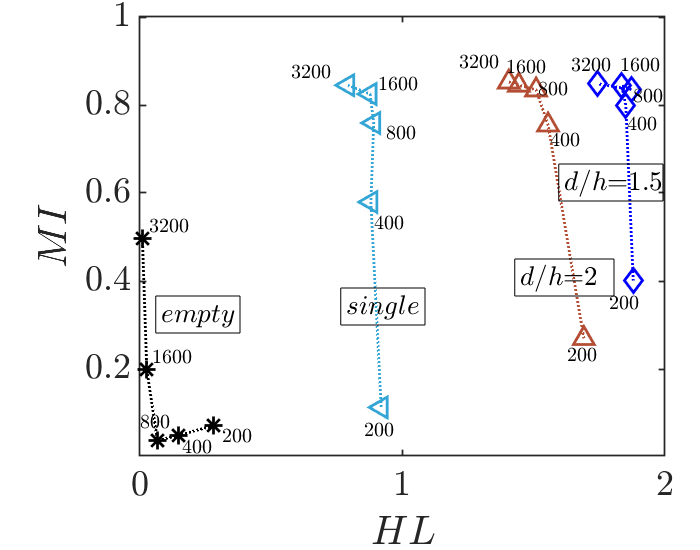
\includegraphics[width=1\linewidth,trim=0.5cm 0cm 0cm 0cm,clip]{Figures/MI_HL/Zoom1_MI_HL_12h.png}
					\begin{overpic}[width=1\linewidth,trim=0.5cm 0cm 0cm 0cm,clip]{Figures/MI_HL/Zoom1_MI_HL_12h.png}
						%	\put(0,185){{\parbox{1\linewidth}{$(a)$}}}	
					\end{overpic}
				\end{minipage}
				\begin{minipage}[c]{0.48\linewidth}
					\begin{overpic}[width=1\linewidth,trim=0.5cm 0cm 0cm 0cm,clip]{Figures/MI_HL/Zoom2_MI_HL_12h.png}
						%					\put(0,185){{\parbox{1\linewidth}{$(b)$}}}	
					\end{overpic}
				\end{minipage}\vspace{0cm}
			\end{center}
			\caption{Zoom-in of clusters of data points shown in Figure \ref{fig:MImax_HL}(a). $Re$ value is shown near each data point.}
			\label{fig:MImax_HL2_zoom}
		\end{figure}
		
						
		\begin{figure}[h]
			\begin{center}
				\begin{minipage}[c]{0.55\linewidth}
					%				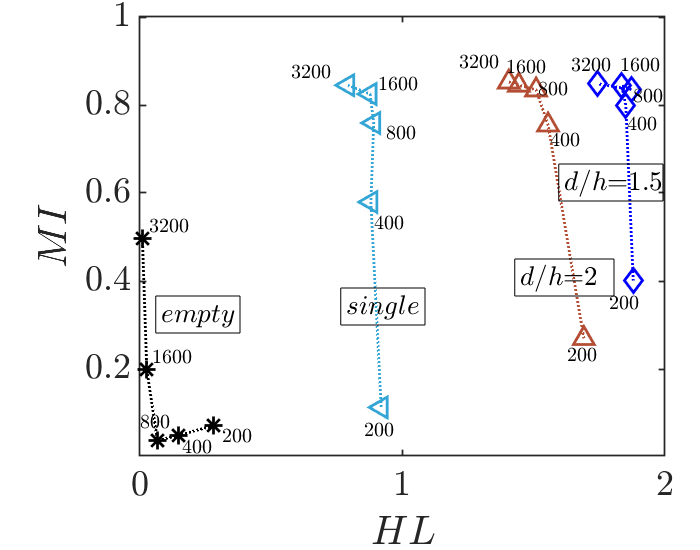
\includegraphics[width=1\linewidth,trim=0.5cm 0cm 0cm 0cm,clip]{Figures/MI_HL/Zoom1_MI_HL_12h.png}
					\begin{overpic}[width=1\linewidth,trim=0cm 0cm 0cm 0cm,clip]{Figures/mesh_U.png}
						%	\put(0,185){{\parbox{1\linewidth}{$(a)$}}}	
					\end{overpic}
				\end{minipage}
				\begin{minipage}[c]{0.4\linewidth}
					\begin{overpic}[width=1\linewidth,trim=0cm 0cm 0cm 0cm,clip]{Figures/mesh_def.png}
						%					\put(0,185){{\parbox{1\linewidth}{$(b)$}}}	
					\end{overpic}
				\end{minipage}\vspace{0cm}
			\end{center}
			\caption{Grid independence results for plates' tip deflection at three different mesh densities.}
			\label{fig:grid}
		\end{figure}
		
				\setstretch{1}
		\bibliographystyle{cas-model2-names}
		% Loading bibliography database
		\bibliography{pre2.bib}
		
	\end{document}
